\documentclass{pracamgr}

\usepackage{polski}

\usepackage[latin2]{inputenc}
\usepackage{pdfpages}
\usepackage{listings}
\usepackage{moreverb}

\vbadness=10000
\hbadness=10000

\author{Piotr Adam Tabor}

\nralbumu{214569}

\title{Projekt i implementacja protoko�u sieciowego dla semistrukturalnej bazy
danych}

\tytulang{Design and development of network protocol for semistructured DBMS}

\kierunek{Informatyka}

\opiekun{dra hab. Krzysztofa Stencla}

% miesi�c i~rok:
\date{Maj 2008}

%Poda� dziedzin� wg klasyfikacji Socrates-Erasmus:
\dziedzina{ 
11.3 Informatyka\\ 
}

 

%Klasyfikacja tematyczna wedlug AMS (matematyka) lub ACM (informatyka)
%http://www.acm.org/class/1998/ccs98.html
\klasyfikacja{C. Computer Systems Organization\\
  C.2 Computer-communication networks\\
  C.2.2 Network Protocols \\
  Applications (SMTP, FTP, etc.)}

% S�owa kluczowe:
\keywords{Protok� sieciowy, \loxim, SBQL, SBA, bazy danych, podej�cie stosowe,
LDAP, generowanie kodu, ASN.1}

% Tu jest dobre miejsce na Twoje w�asne makra i~�rodowiska:
\newtheorem{defi}{Definicja}[section]


% koniec definicji

%=============================== MAKRA  =====================================

\newcommand{\loxim}{LoXiM}
\newcommand{\patrz}[1]{(patrz: \ref{#1})}

%============================================================================

%% Tabelka o znaczeniu poszczeg�lnych bajt�w w protokole
\newenvironment{bajty}{\\ \begin{tabular}{|l|l|l|}\hline
{\bf{Od - do}} & {\bf{Typ/Warto��}} & {\bf{Zawarto��}} \\\hline}{\hline\end{tabular}\\\\} % item


\newcommand{\bp}[4]{\parbox[t]{2.5cm}{#1 $\rightarrow$ #2} & \parbox[t]{3cm}{#3\\} & \parbox[t]{10cm}{#4\vspace{1em}}
\\ } 

\newcommand{\znacznik}[1]{$<$#1$>$}
%% Tabelka o znaczeniu poszczeg�lnych bajt�w w protokole
\providecommand{\znakzero}{$\backslash 000$}

\newenvironment{bajtyo}{\\
\begin{tabular*}{16.775cm}{|p{4.5cm}|p{4cm}|p{7cm}|}\hline {\bf{Od - do}} &
{\bf{Warto��}} & {\bf{Zawarto��}} \\\hline}{\hline\end{tabular*}} % item
\providecommand{\bpo}[4]{#1 $\longleftrightarrow$ #2 & #3 & \parbox[t]{7cm}{#4}
\\ }


\begin{document}

%Tytu�y dodatk�w
\newcommand{\dokoldtcpproto}{Analiza zastanego protoko�u sieciowego w bazie danych \loxim}
\newcommand{\doknewtcpproto}{Protok� komunikacyjny dla bazy danych
\loxim{} - wersja 2.0}
\newcommand{\dokprotogen}{ProtoGen~1.0 - dokumentacja generatora protoko��w
sieciowych}
\newcommand{\doksbqlvialdap}{Analiza mo�liwo�ci wykorzystania protoko�u LDAP dla
SBQL DB}

\maketitle

%tu idzie streszczenie na strone poczatkowa
\begin{abstract}
Poni�sza praca opisuje projekt polegaj�cy na wymianie protoko�u sieciowego w
semistrukturalnej bazie danych \loxim. Zawiera dokumentacj� poszczeg�lnych
krok�w tego zagadnienia: analiz� i wskazanie wad architektonicznych i
implementacyjnych w zastanym protokole, projekt nowego rozwi�zania, a tak�e
implementacj� generatora kod�w �r�d�owych protoko��w sieciowych pewnej
klasy na podstawie danego pliku XML dla najbardziej popularnych j�zyk�w
programowania - C++ i Javy.

% W pracy w szczeg�lno�ci om�wiono zagadnienie wydajnej wymiany danych o
% z�o�onej strukturze (drzewa ze wska�nikami) pomi�dzy systemami informatycznymi z
% uwzgl�dnieniem problem�w wynik�ych z r�nic zar�wno technicznych (architektura procesora) jak i
% logicznych (r�ne j�zyki programowania).
\end{abstract}

\tableofcontents
%\listoffigures
%\listoftables

\chapter{Wprowadzenie}
\addcontentsline{toc}{chapter}{Wprowadzenie}

Praca to opisuje przebieg projektu polegaj�cego na wyspecyfikowaniu i
zaimplementowaniu protoko�u sieciowego dla bazy danych \loxim, kt�ra to baza
powstaje pod kierownictwem dr hab. Krzysztofa Stencla na Wydziale
Matematyki, Informatyki i Mechaniki Uniwersytetu Warszawskiego. 

Dokument ten omawia zagadnienie protoko��w sieciowych w zakresie warstwy
g�rnej modelu OSI (Open System Interconnection) \cite{OSI}, czyli:
	\begin{itemize}
      \item 5. Warstwy sesji
      \item 6. Warstwy prezentacji
      \item 7.	Warstwy aplikacji 
    \end{itemize}	 
Zakres ten jest to�samy z zakresem ,,Warstwy aplikacji'' w modelu DoD
(Department of Defense) \cite{DoD}.

Praca ta - jako ca�o�� -  toczy�a si� do�� d�ugo. Pierwsze jej elementy
powsta�y na jesieni roku 2006, ale mimo wszystko uda�o si� utrzyma� zgodno��
finalnego dzie�a z aktualnymi potrzebami, a nawet zaimplementowany protok�
przewiduje obs�ug� wielu funkcjonalno�ci i zastosowa� nieobecnych jeszcze w
systemie \loxim{} w momencie oddania pracy. W sekcji \ref{cel} znajduj� si� informacje o zakresie zrealizowanego
projektu.

W trakcie przebiegu tej pracy powsta�o kilka dokument�w, kt�re
dobrze spe�niaj� swoj� rol� jako dzie�a oddzielne - skierowane do 
czytelnika zainteresowanego szczeg�lnymi aspektami tej pracy i z tego wzgl�du 
zamieszczam je jako dodatki do tego dokumentu. Opis tych element�w
sk�adowych znajduje si� w sekcji \ref{elementy_skladowe}.

Bezpo�rednio w tym dokumencie chc� si� skupi� na kwestii przebiegu tej pracy,
uzasadnieniu podj�tych istotnych decyzji projektowych i rozwa�eniu trudno�ci z
kt�rymi si� spotka�em.  Nast�pne rozdzia�y po�wi�cam zatem rozwa�aniom
dotycz�cym poszczeg�lnych faz projektu: 
\begin{description}
	\item[Analizie zastanego protoko�u w bazie \loxim] - rozdzia�: \ref{analiza}
	\item[Projekt nowego protoko�u dla bazy \loxim] - rozdzia�: \ref{projekt}
	\item[Implementacji nowego protoko�u dla bazy \loxim] - rozdzia�:
	\ref{implementacja}
	\item[Implementacja generatora protoko��w dla bazy \loxim] - rozdzia�:
	\ref{generator}
	\item[Przeprowadzone testy] - rozdzia�: \ref{testy}
\end{description}

Dokument ten zosta� wi�c zorganizowany niemal chronologicznie, a zarazem
zgodnie z przebiegiem prac. W niekt�rych tylko miejscach pozwoli�em sobie zawrze� wnioski,
kt�re wynik�y z mojego p�niejszego do�wiadczenia, ale kt�re tematycznie
powinny zosta� uwzgl�dnione na danym etapie realizacji projektu. 

Ca�o�� tre�ci w�a�ciwej zamyka podsumowanie w rozdziale: \ref{podsumowanie}.

W dodatkach - opr�cz om�wionych w nast�pnym rozdziale dokument�w - znajduje si�
spis tre�ci za��czonej p�yty CD (dodatek \ref{spis-tresci-cd}).

\section{Elementy sk�adowe pracy magisterskiej} \label{elementy_skladowe}

Opr�cz poni�szego dokumentu w sk�ad pracy zosta�y w��czone nast�puj�ce
dokumenty:
\subsection{,,\dokoldtcpproto''} 
	Dodatek \ref{dokoldtcpproto}

	Dokument opisuje protok� sieciowy jaki zasta�em w bazie danych
	\loxim{} w pa�dzierniku 2006 roku. Dokument by� pisany w kontek�cie rozpoznania
	protoko�u na potrzeby stworzenia sterownika JDBC jego u�ywaj�cego ---
	co by�o moim pierwotnym zamierzeniem. Krytyka rozwi�zania zawarta w tym 
	dokumencie sta�a si� przyczyn� podj�cia decyzji o wymianie protoko�u w bazie
	\loxim{} na nowy.
\subsection{,,\doknewtcpproto''}
	Dodatek \ref{doknewtcpproto}

	Dokument ten realizuje dwa istotne cele: 
	\begin{itemize}
      \item Stanowi� swojego rodzaju ,,zam�wienie'', czyli przedstawia�
      kontrakt jaki protok� b�dzie realizowa�, co u�atwia�o rozmowy z
      autorami innych modu��w systemu \loxim{} oraz kierownikiem projektu i
      umo�liwia�o wykrycie brak�w funkcjonalnych b�d� zagro�e�. 
      \item Aktualnie stanowi on dokumentacj� obecnego protoko�u w bazie danych
      \loxim. Jest dokumentem, kt�ry ka�da osoba chc�ca napisa� narz�dzie bezpo�rednio 
      komunikuj�ce si� z systemem \loxim{} musi przeczyta� i dokument ten
      powinien odpowiedzie� na wszelkie pytania dotycz�ce tego interfejsu. 
      \end{itemize}
\subsection{,,\doksbqlvialdap''}
	Dodatek \ref{doksbqlvialdap}

	Dokument ten rozwa�a kwestie mo�liwo�ci wykorzystania protoko�u LDAP do
	komunikacji z baz� danych opart� o j�zyk SBQL. Zainspirowany zosta� pozornie
	podobnym modelem danych i wykazuje powa�ne trudno�ci (mimo licznych
	podobie�stw) w integracji obu rozwi�za�. 
\subsection{,,\dokprotogen''}
	Dodatek \ref{dokprotogen}
	
	Tekst ten stanowi pe�n� dokumentacj� narz�dzia, kt�re umo�liwia wygenerowanie
	na podstawie zadanego deskryptora protoko�u w formacie XML, jego implementacj� 
	w wybranym j�zyku programowania. Dokument omawia zar�wno spos�b u�ycia tego
	narz�dzia jak i porusza kwestie jego wewn�trznej architektury oraz mo�liwo�ci
	dalszej rozbudowy. 
\newpage
\section{Cel} \label{cel}

Pierwotnym zagadnieniem, kt�rym chcia�em si� zaj�� w ramach pracy
magisterskiej, by�o zbudowanie odpowiednika ORM (Object-Relational mapping) dla
bazy \loxim{} w Javie. Okaza�o si� jednak, �e baza danych \loxim{} nie posiada
sterownika JDBC, kt�ry by umo�liwia� zastosowanie standardowych dla Javy metod
��czno�ci z bazami danych. Dlatego zainteresowa�em si� stworzeniem sterownika
JDBC dla \loxim'a. Niestety przeprowadzona analiza zastanego protoko�u
\patrz{analiza} wykaza�a, �e obecny protok� jest ca�kowicie nieu�yteczny. W
zwi�zku z tym, celem tej pracy sta�a si� wymiana protoko�u w systemie \loxim{}
na istotnie lepszy. Rozumiemy przez to: 
 
	\begin{itemize}
      \item Uzyskanie stabilnego, bezpiecznego protoko�u- umo�liwiaj�cego pe�ne
      wykorzystanie obecnych i potencjalnie przysz�ych mo�liwo�ci systemu \loxim
      - autentykacji, przesy�ania zapyta� i uzyskiwania z�o�onych odpowiedzi,
      przerywania zapyta� w trakcie ich wykonania,a tak�e konfiguracji sesji z
      baz� danych. 
     
      \item Uzyskanie protoko�u potrafi�cego pracowa� pomi�dzy maszynami o
      r�nych architekturach sprz�towych i programowych.
     
      \item Uzyskanie efektywnego (pod wzgl�dem wykorzystania sieci i CPU) 
      i �atwo rozszerzalnego protoko�u.
      
      \item Modu�y protoko�u powinny stanowi� wygodny i sp�jny interfejs -
      mo�liwie zgodny z dobr� praktyk� programowania w j�zyku dla kt�rego
      zosta�y przygotowane. W szczeg�lno�ci w j�zykach ze statyczn� kontrol�
      typ�w pakiety danych powinny jej podlega�.  
      
      \item Przygotowanie do implementacji sterownika JDBC w oparciu o ten
      protok�.
    \end{itemize}
    
    W trakcie prac nad systemem sta�o si� oczywiste jeszcze jedno wymaganie - 
    potrzebna jest implementacja tego protoko�u w wielu j�zykach programowania:
    \begin{description}
		\item[C++] - ze wzgl�du na to, �e \loxim{} jest napisany w j�zyku C++
		\item[Java]- ze wzgl�du na to, �e sterownik JDBC musi zosta� napisany w Javie
		\item[.NET (C\#)] - ze wzgl�du na to, �e w maju 2007 powsta�a istotna cz��
		serwera \loxim{} zaimplementowana w j�zyku C\#
		\item[itd.] 
    \end{description}
    Realizacja wsparcia dla wielu j�zyk�w sta�a si� przyczyn� stworzenia
    generatora protoko��w \patrz{generator}.
    

\chapter{Analiza zastanego protoko�u} \label{analiza}
W pa�dzierniku 2006 roku - kiedy przyst�powa�em do pracy z systemem \loxim{} -
nie istnia�a �adna dokumentacja, ani opis u�ywanego przez ten system protoko�u
sieciowego. By�y wi�c konieczno�ci� - na podstawie kodu �r�d�owego -
przeprowadzenie audytu tego jedynego (pomijaj�c standardowe wyj�cie) interfejsu
komunikacyjnego bazy danych ze �wiatem zewn�trznym. 

Opis ten zosta� zawarty w dokumencie ,,\dokoldtcpproto'' (dodatek
\ref{dokoldtcpproto}).

\section{Wnioski z przeprowadzonej analizy}
Przytocz� w tym dokumencie wnioski, kt�re wyp�yn�y z przeprowadzonego
przeze mnie audytu:
%& --translate-file latin2pl
\providecommand{\znakzero}{$\backslash 000$}

	\begin{itemize}
      \item Protok� ten nie b�dzie dzia�a� pomi�dzy komputerami r�ni�cymi
      si� architektur� lub trybem kompilacji (big endian - little 
      endian), (8, 16, 32, 64 bity).
      
      \item Brak okre�lonych z g�ry rozmiar�w pakiet�w i ich element�w - co
      utrudnia stronie odbieraj�cej alokowanie bufor�w o odpowiednich
      rozmiarach.

      \item Brak mo�liwo�ci przerwania zleconego zapytania w trakcie jego 
	wykonania     

      
      \item Ka�dy pakiet ma inn� konstrukcj� i   spos�b zapisywania tre�ci. 
      
      \item Brak negocjacji wst�pnych przy nawi�zywaniu po��czenia (logowanie,
      por�wnanie wersji, synchronizacja czasu, strona kodowa znak�w w
      �a�cuchach)
      
      \item Generalny brak konsekwencji.
      
      Czasami kod korzysta z funkcji zawartych w pliku TCPIP.cpp,a innym razem
      realizuje ca�kowicie analogiczn� operacje bezpo�rednio. 
      
      Dla przyk�adu - pola tekstowe s� przesy�ane na jeden z 3 sposob�w:
      \begin{itemize}
      	\item Jako ci�gi bajt�w, poprzedzone liczb� �wiadcz�c� o ich d�ugo�ci
      	(wliczaj�c znak \znakzero{} na ko�cu). 
      	\item Jako ci�gi bajt�w, poprzedzone liczb� �wiadcz�c� o ich d�ugo�ci
      	(nie wliczaj�c znak \znakzero{} na ko�cu).
      	\item Jako ci�gi bajt�w - z za�o�eniem, �e znak \znakzero{} ko�czy
      	przesy�any napis.
      \end{itemize}
      
      \item Brak organizacji wewn�trznej pakiet�w umo�liwiaj�cej wygodn�
      rozbudow� protoko�u (o nowe dane w poszczeg�lnych pakietach)
      
      \item Obs�uga maksymalnie maxint+1 obiekt�w (czyli np. 32768 na
      architekturach 16-bitowych). 
      
      \item Protok� nie przewiduje mo�liwo�ci przesy�ania liczb ca�kowitych
      ujemnych.
  
      \item Duplikacja kodu - wiele fragment�w kodu jest skopiowanych
      (copy-paste) z innego miejsca. Mo�na by tego unikn�� organizuj�c kod
      w odpowiedni spos�b. 
 
	  \item Istniej� trzy typy zwi�zane z przesy�aniem danych logicznych:
		Result::BOOLTRUE, Result::BOOLFALSE, Result::BOOL - ka�dy serializowalny z   
		innym identyfikatorem. Prawdopodobnie kt�ry� z nich powsta� przez pomy�k�.
    \end{itemize}


W wyniku tej krytyki zosta�a podj�ta decyzja o zaprojektowaniu i wykonaniu
nowego - pozbawionego powy�szych wad - protoko�u komunikacyjnego dla
\loxim{}'a.

\chapter{Projekt nowego protoko�u}	\label{projekt}

\section{Wyb�r klasy protoko�u}
Kluczow� decyzj� przy projektowaniu nowego protoko�u komunikacyjnego, by�o
podj�cie decyzji o jego typie. Poni�ej spr�bujemy przejrze� dost�pne
mo�liwo�ci i rozwa�y� ich wady i zalety:

\subsection{Klasyczne protoko�y tekstowe}\label{proto_txt} 
Przyk�adami klasycznych protoko��w tekstowych s� protoko�y: HTTP, FTP,
NNTP, POP3, SMTP.
S� to protoko�y w kt�rych wszystkie polecenia  i odpowiedzi
s� zapisywane w postaci tekstowych komend. S� one charakterystyczne dla wczesnego etapu rozwoju komunikacji w sieciach komputerowych, g��wnie ze wzgl�du na poni�sze zalety:
\begin{itemize}
  \item Mo�liwo�� bezpo�redniej komunikacji cz�owieka z urz�dzeniem przy pomocy
  	     tekstowego protoko�u (wystarczy narz�dzie typu ,,netcat'')
  \item Brak problem�w z wymian� danych pomi�dzy urz�dzeniami r�nego typu i o
  r�nych architekturach (big/little endian, d�ugo��
  s�owa procesora). Przewa�nie wymagane jest jedynie aby oba urz�dzenia
  honorowa�y standard ASCII w zakresie znak�w o kodach $0-127$).
  \item Mo�liwo�� bezpo�redniego logowania komunikacji na drukark�. 
  \item Du�a �atwo�� szukania b��d�w. 
\end{itemize}

Niestety posiadaj� one tak�e wiele wad:
\begin{itemize}
  \item Wysoki narzut na transmisj� danych (w kategoriach rozmiaru przes�anych
  danych). Np. wys�anie liczby 17-to cyfrowej wymaga w protokole binarnym 8
  bajt�w, a w protokole tekstowym 17 bajt�w. 
  \item Konieczno�� parsowania i budowania komunikat�w tekstowych (ma�o wygodne dla programisty oraz wprowadzaj�ce istotny narzut
  obliczeniowy).
  \item Trudno�� przesy�ania danych o z�o�onej strukturze. 
\end{itemize}

\subsection{Protoko�y oparte na XML} \label{proto_xml}
Przyk�adem takiego protoko�u jest protok� XMPP (Extensible Messaging and
Presence Protocol) wykorzystywane przez komunikatory internetowe
(jabber, gtalk).  

Protoko�y tego typu posiadaj� wi�kszo�� zalet protoko��w tekstowych
\patrz{proto_txt}. Jedynie czytelno�� i mo�liwo�� bezpo�redniej obs�ugi protoko�u przez cz�owieka uleg�a
	obni�eniu. Ponadto do zalet nale�y doliczy�:
	\begin{itemize}
      \item mnogo�� narz�dzi umo�liwiaj�cych np. automatyczn� kontrol�
      poprawno�ci komunikat�w (XML Schema) lub przekszta�canie komunikat�w z
      jednej postaci na drug� (XSLT). 
      \item obecno�� wielu ,,standard�w'' wymiany tre�ci okre�lonego typu
      \item obs�ug� wielu kodowa� znak�w.
      \item mo�liwo�� wymiany danych o z�o�onej strukturze, 
    \end{itemize}
    
   W wadach istotne pozostaj� dwie charakterystyczne dla protoko��w tekstowych:
    \begin{itemize}
  		\item Wysoki narzut (w kategoriach wykorzystania sieci) na transmisj�
  	danych.
  		\item Konieczno�� parsowania komunikat�w i narzut obliczeniowy z tym
  		zwi�zany (istotnie mniejszy ni� w przypadku klasycznej komunikacji
  		tekstowej). 
    \end{itemize} 
    
    \subsubsection{Protoko�y XML oparte na RPC (Remote Procedure Call) - np.
    XML-RPC, SOAP, Web-Services} 
    
    Nale�y w szczeg�lny spos�b wyr�ni� zestandaryzowan� klas� protoko��w
    sieciowych zwi�zanych ze zdalnym wywo�ywaniem procedur i stanowi�cych
    obecnie powszechnie u�ywany standard w komunikacji sieciowej pomi�dzy
    r�nymi systemami tzw. Web-Services.
    
    Wszystkie one wyr�niaj� w komunikacji stron� zadaj�c� zapytanie (request)
    i stron� udzielaj�c� odpowiedzi (response). Strona udzielaj�ca odpowiedzi
    udost�pnia metod� (zawieraj�c� potencjalnie z�o�one - obiektowe -
    parametry), kt�ra poprzez odpowiednio sformatowane zapytanie jest
    uruchamiana. Warto�� wynikowa wykonanej metody jest kodowana w postaci
    XML'a i zwracana do strony pytaj�cej.
    
    Zalet� tych protoko��w jest bez w�tpienia:
    \begin{itemize}
    	 \item jeszcze wi�ksze zestandaryzowanie (WSDL) 
    	 \item du�a ilo�� narz�dzi wspieraj�cych u�ytkowanie tych protoko��w
    	 \item Istnienie generator�w kodu, kt�re na podstawie opisu takiego
    	 protoko�u (WSDL) generuj� dla wielu j�zyk�w programowania kod potrzebny
    	 do komunikacji. 
    	 \item U�ywanie portu 80 i warstwy transportu opartej o HTTP, co umo�liwia
    	 unikni�cie problem�w zwi�zanych z dzia�aniem zap�r sieciowych i 
    	 szczeg�lnych polityk bezpiecze�stwa.    
    \end{itemize}
    
    Niestety wprowadzaj� one te� pewne istotne wady:
    \begin{itemize}
      \item S� bezpo��czeniowe - wymagaj� nawi�zania po��czenia i
      przeprowadzenia procesu autoryzacji przy ka�dym wywo�aniu - co ma bardzo
      negatywny wp�yw na wydajno�� i bezpiecze�stwo, a tak�e mo�e spowodowa�
      ograniczenie komunikacji przez urz�dzenia sieciowe (zbyt wiele ��da�
      w zadanym okresie czasu). 
      \item Wyr�niaj� stron� zadaj�c� pytanie i na ni� odpowiadaj�c�.
      Komunikacja dwustronna wymaga tego, aby obie strony umia�y
      zainicjalizowa� po��czenie - co w przypadku sieci opartych np. o
      maskarad� IP mo�e by� trudne lub nawet niemo�liwe. 
    \end{itemize}
    
\subsection{Protoko�y binarne oparte na RPC}
	Istnieje wiele rozwi�za� zdalnego wywo�ywania procedur pomi�dzy komponentami w
sieciach komputerowych wykorzystuj�cych komunikacj� binarn�. Mechanizmem, kt�ry
powinien umo�liwi� stworzenie takiego rozwi�zania jest standard CORBA (Common
Object Request Broker Architecture). Teoretycznie powinien on umo�liwi� wygenerowanie
na podstawie zadanego IDL'a (Interface Description Language) implementacji
protoko�u dla wielu r�nych j�zyk�w programowania. Niestety rzeczywisto��
pokazuje, �e nie istnieje dobra - niekomercyjna - implementacja standardu
CORBA (http://www.puder.org/corba/matrix/).

Pozosta�e protoko�y - takie jak RMI (Remote Method Invocation) oraz AMF (Action
Message Format) s� zwi�zane z konkretnymi j�zykami programowania (w tym
przypadku odpowiednio Java i ActionScript). 

\subsection{Protoko�y oparte na ASN.1 (Abstract Syntax Notation One)}\label{ASN1}

ASN.1 jest standardem s�u��cym do opisu metod kodowania, dekodowania i
przesy�ania danych. Jest to obecnie standard ISO/IEC 8824. Pozwala on
zdefiniowa� za pomoc� sformalizowanego opisu sk�adnie p�l w
komunikatach, a nast�pnie wygenerowa� kod seralizuj�cy i deserializuj�cy te
pakiety. 

Standard ASN.1 nie definiuje bezpo�rednio binarnego formatu przesy�anych
komunikat�w. Mog� by� one serializowalne wed�ug jednej z zaproponowanych
zasad (encoding rules). W szczeg�lno�ci istniej� trzy najpopularniejsze
mo�liwo�ci w tej kwestii: 
\begin{description}
\item[BER] - (Basic encoding rules) - zapami�tuje ka�de pole w postaci
binarnej jako tr�jk�: znacznik, d�ugo��, warto��.
\item[PER] - (Packed encoding rules) - podobnie jak BER, ale metoda bardzo
zwraca uwag� na efektywno�� pod wzgl�dem rozmiaru pakiet�w.  
\item[XER] (XML encoding rules) - komunikaty s� przesy�ane w postaci paczek
XML. 
\end{description} 

Mo�na ten standard por�wna� do zaprezentowanego w ramach tej pracy
generatora protoko��w. 

\subsubsection{Protok� LDAP (Lightweight Directory Access Protocol)}

Szczeg�lnym przypadkiem protoko�u opartego na standardzie ASN.1 jest protok�
LDAP (Lightweight Directory Access Protocol) s�u��cy do wymiany danych z us�ugami
katalogowym (Directory Services). Ze wzgl�du na podobne zastosowanie
(uzyskiwanie dost�pu do bazy danych o hierarchicznej strukturze) wyda�a mi si� 
warta g��bszej analizy kwestia rozwa�enia mo�liwo�ci wykorzystania tego
protoko�u (z ewentualnymi rozszerzeniami) - jako protoko�u do bazy danych \loxim. 

Problematyk� t� szczeg�owo omawia za��czony do tej pracy dokument mojego
autorstwa pt.: ,,\doksbqlvialdap'' (patrz dodatek \ref{doksbqlvialdap}).

\subsection{Protoko�y dedykowane}
S� to protoko�y binarne specjalnie zaprojektowane do konkretnych rozwi�za�. 

\subsection{Wnioski}
	Z protoko��w tekstowych najlepiej nadawa�by si� do omawianego zastosowania 
	protok� oparty na XML, ale nie b�d�cy us�ug� ,,Web-Service'' (zdyskwalifikowany
	ze wzgl�du na bezpo��czeniowo��). 
	
	Jednak wysoki narzut zwi�zany zar�wno z transmisj� jak i parsowaniem
	danych przewa�y� decyzj� na rzecz protoko��w binarnych (wyzwaniem postawionym
	 bazie danych \loxim{} jest udowodnienie, �e
	obiektowe/semistrukturalne bazy danych mog� konkurowa� pod wzgl�dem wydajno�ci
	z bazami relacyjnymi, wi�c nie chcieli�my wprowadzi� w�skiego gard�a na
	poziomie tego komponentu systemu).
	
	Dysponuj�c obecn� wiedz�, dla systemu LoXiM zaleci�bym z pewno�ci� protok�
	zbudowany w oparciu o standard ASN.1 \patrz{ASN1}. Pozwoli�oby to pozosta� 
	w pe�ni zgodnym ze standardami ISO, a tak�e unikn�� istotnej cz�ci
	implementacji - pos�uguj�c si� kt�rym� z generator�w kodu dla standardu ASN.1.
	
	Protok� ten zosta�by zapewne oparty na kanwie protoko�u LDAP (analogiczna
	konstrukcja paczek, zgodna autoryzacja), ale do przesy�ania zapyta� i odczytywania
	ich wynik�w zaproponowa�bym w�asne paczki - semantycznie zgodne z tymi
	zaproponowanymi w sekcjach \ref{proto_obsluga_zapytan} i
	\ref{proto_obsluga_wartosci}.

	Podejmuj�c t� decyzj� projektow� w grudniu 2006 roku, odrzuci�em
	protok� tekstowy ze wzgl�du na zbyt nisk� wydajno��, a tak�e u�ycie CORBY ze
	wzgl�du na niesatysfakcjonuj�c� jako�� bezp�atnych produkt�w i w ten spos�b
	zdecydowa�em si� zaprojektowa� protok� dedykowany. 


\section{Projekt dedykowanego protoko�u}

	Projekt, a tym samym dokumentacja dedykowanego protoko�u sieciowego dla bazy
	danych \loxim{} znajduje si� w za��czniku do tej pracy zatytu�owanym: ,,\doknewtcpproto''.
	Dokument ten szczeg�owo omawia kwestie takie jak:
	\begin{itemize}
      \item Format binarny poszczeg�lnych pakiet�w
      \item Dozwolone sekwencje wymiany pakiet�w
      \item Metody autoryzacji
      \item Kwestie bezpiecze�stwa w sieci
      \item Podzia� protoko�u na warstwy logiczne
      \item Problemy zwi�zane z danymi regionalnymi, takimi jak strefy czasowe,
      metody por�wnywanie napis�w.
    \end{itemize}
	
\chapter{Implementacja protoko�u} \label{implementacja}
	Po przedstawieniu ,,Projektu protoko�u sieciowego dla bazy danych \loxim'' i
om�wieniu go na seminarium - zosta�y wprowadzone do niego niewielkie zmiany i
w tej postaci zosta� skierowany do realizacji. 

	Jako, �e system \loxim{} jest napisany w j�zyku C++, kluczowa by�a implementacja
protoko�u w tym w�a�nie j�zyku programowania. Protok� uda�o si�
zaimplementowa� dokonuj�c tylko kosmetycznych zmian w stosunku do pierwotnego
projektu. 

	Istotn� cz�ci� tej implementacji by�o stworzenie wygodnego - obiektowego -
API do obs�ugi strumieni i gniazd sieciowych. Implementuj�c je wzorowa�em si�
w istotnym stopniu na tym udost�pnianym przez klasy w j�zyku Java takie jak:
InputStream, OutputStream, Socket, ClientSocket i ServerSocket.

Opis tej implementacji protoko�u mo�na znale�� w rozdziale: 3.2 ,,Wygenerowany
kod dla j�zyka C++'' dokumentu ,,\dokprotogen'' (dodatek \ref{dokprotogen}), ze
wzgl�du na to, �e ten kod zosta� wykorzystany jako baza dla generowanego kodu do j�zyka C++. 

\chapter{Generator implementacji protoko��w}\label{generator}

\section{Geneza}
Implementuj�c protok� w C++, stwierdzi�em, �e ponad 70\% czasu zaj�o mi 
do�� mechaniczne tworzenie kodu poszczeg�lnych pakiet�w, a pozosta�e 30\%
czasu powstawa� kod, kt�ry by� niemal niezale�ny od protoko�u z kt�rym mia�em
do czynienia.

Ponadto - w maju 2007 roku - gdy sko�czy�em implementacje protoko�u w j�zyku
C++ - pojawi� si� zacz�tek implementacji serwera \loxim{} w j�zyku C\# na
platformie Microsoft .NET. Widz�c wi�c potrzeb� stworzenia implementacji tego
protoko�u w dw�ch kolejnych j�zykach programowania (C\# i Java na potrzeby
sterownika JDBC), a tak�e konieczno�� utrzymania tych 3 implementacji sp�jnymi
przy wszelkich modyfikacjach, doszed�em do wniosku, �e nieodzowne wydaje si�  
stworzenie generatora implementacji protoko�u wedle zadanego jego opisu. 

\section{Opis}
W dokumencie ,,\dokprotogen'' (dodatek \ref{dokprotogen}) 
znajduje si� dokumentacja zar�wno u�ytkowa jak i programistyczna tego
narz�dzia. Program ten (napisany w Javie) zawiera obecnie modu�y
generuj�ce kod do j�zyka C++ i do j�zyka Java, ale posiada mo�liwo�� �atwego
rozbudowania o producent�w kodu do kolejnych j�zyk�w programowania.

Zaimplementowany generator wraz z plikami �r�d�owymi znajduje si� na za��czonej
do pracy p�ycie CD-ROM w katalogu ``/protogen''. 

Jako ciekawostk� chcia�bym zwr�ci� uwag� na r�nic� w ilo�ci kodu �r�d�owego,
kt�ry by� potrzebny do napisania modu��w generatora (o ca�kowicie zgodnej
funkcjonalno�ci) :

\begin{description}
	\item[Modu� generuj�cy kod do C++] 84 785 bajt�w kodu �r�d�owego
	\item[Modu� generuj�cy kod do Javy] 56 091 bajt�w kodu �r�d�owego
\end{description}

Czyli kod generuj�cy do j�zyka C++ jest o 50\% d�u�szy od kodu generuj�cego do
j�zyka Java. Proporcja ta wynika g��wnie z konieczno�ci generowania plik�w
nag��wkowych dla j�zyka C++. 

\section{Wygenerowany kod dla LoXiM'a}

W katalogu ``/protogen/example'' 
za��czonej p�yty zosta� umieszczony pe�en zbi�r plik�w potrzebnych do
wygenerowania kompletnego protoko�u dla C++ i Javy. Opr�cz pliku xml 
deskryptora stanowi� go r�cznie przygotowane pliki dw�ch paczek: 
CollectPackage i Q\_c\_executePackage, kt�rych logika by�a na tyle skomplikowana,
�e generator implementacji protoko�u ,,ProtoGen~1.0'' jej obecnie nie wspiera.

Aby r�cznie przeprowadzi� proces generowania kodu, najlepiej jest:
\begin{enumerate}
\item skopiowa� na
dysk lokalny ca�y katalog /protogen z za��czonej p�yty CD (podkatalog
/protogen/src jest zb�dny). 
\item upewni� si�, �e posiadamy prawa zapisu do skopiowanego podkatalogu
./protogen/example. Ewentualnie nada� odpowiednie przywileje. 
\item uruchomi� program ./protogen/example/run.sh
\end{enumerate}
 
W katalogu ./protogen/example/result-cpp i ./protogen/example/result-java
powinny zosta� wygenerowane implementacje protoko�u.

Por�wnanie ilo�ci wygenerowanego kodu (klasy paczek i typy wyliczeniowe) dla
obu protoko��w sieciowych pokazuj� podobny wynik: 
\begin{description}
	\item[Wygenerowany kod dla C++] 131 278 bajt�w kodu �r�d�owego
	\item[Wygenerowany kod dla Javy] 120 591 bajt�w kodu �r�d�owego
\end{description}
  
Opr�cz tego - dla obu j�zyk�w - zosta�y wygenerowane oko�o 850KB pliki
zawieraj�ce testowe instancje pakiet�w \patrz{testy}. 

Gotowe implementacje protoko�u dla \loxim{}'a s� tak�e za��czone na p�ycie w
katalogu /loxim\_protocol. 

\chapter{Przeprowadzone testy}\label{testy}

\section{Metoda i narz�dzia}

R�cznie napisana implementacja protoko�u w j�zyku C++ zawiera�a przyk�adowe
scenariusze testowe zaadresowane zar�wno dla strony b�d�cej serwerem jak i dla
strony b�d�cej klientem protoko�u \loxim'a. 

Idea ta zosta�a tak�e przeniesiona do generatora protoko��w ,,ProtoGen~1.0'' w
kt�rym to scenariusze testowe s� przygotowywane automatycznie i s� to�same
pomi�dzy r�nymi docelowymi j�zykami programowania. 

Dla deskryptora protoko�u \loxim'a generator stworzy� opisy 3197
przyk�adowych paczek. Dla j�zyka C++ zosta�y one zawarte w pliku:\\
/loxim\_protocol/cpp/protocol/tests/TestPackagesFactory.cpp \\
a dla j�zyka Java w pliku:\\
/loxim\_protocol/java/src/test/java/pl/edu/mimuw/loxim/protocol/tests/TestPackagesFactory.java.

Dla ka�dego z j�zyk�w programowania jest tworzony program: TestRunnerRec, kt�ry
uruchomiony z parametrem b�d�cym numerem portu - tworzy instancj� serwera
oczekuj�cego na po��czenie na wybranym porcie i sprawdzaj�cego zgodno�ci
otrzymanych pakiet�w z zaplanowanym scenariuszem, oraz program TestRunnerSender,
kt�ry uruchomiony z dwoma parametrami: adresem hosta docelowego i numerem portu na
kt�rym nas�uchuje tam serwer - pod��cza si� do wybranego serwera i wysy�a do
niego paczki wed�ug zadanego scenariusza. 

\section{Sprawdzone przypadki}

Testowe maszyny:
\begin{enumerate}
	\item L64 - Linux 2.6.20, Intel Dual Core - 64 bity, Little-endian  
	\item L32 - Linux 2.6.20, Intel Dual Core - 32 bity, Little-endian
	\item B32 - AIX, Power PC - 32 bity, Big-endian
\end{enumerate}

Sprawdzono, �e system przechodzi testy w nast�puj�cych scenariuszach
\begin{enumerate}
  \item L64 Java $\Longleftrightarrow$ L64 Java 
  \item L64 C++ $\Longleftrightarrow$ L64 C++
  \item L64 C++ $\Longleftrightarrow$ L32 C++
  \item L32 C++ $\Longleftrightarrow$ L32 C++
  \item L32 C++ $\Longleftrightarrow$ L32 Java   
  \item L64 C++ $\Longleftrightarrow$ B32 C++ 
  \item B32 C++ $\Longleftrightarrow$ B32 C++ 
  \item L64 Java $\Longleftrightarrow$ L64 C++
\end{enumerate}

\chapter{Podsumowanie} \label{podsumowanie}

Uwa�am, �e uda�o si� zrealizowa� postawione w pracy cele. Zosta� stworzony
wydajny, przeno�ny, dobrze udokumentowany i dostosowany do obecnych i
przewidywanych przysz�ych potrzeb \loxim{}'a protok� sieciowy. 

Powsta� tak�e uniwersalny generator protoko��w sieciowych - kt�rego pierwotnie
planowany zakres pracy nie dotyczy�. 

W momencie oddawania tej pracy (maj 2008) tocz� si� dwie prace magisterskie w
bardzo istotnym stopniu oparte na wynikach opisanych w tym dokumencie. 
\begin{description}
  \item Praca Marka Dopiery - polegaj�ca na re-implementacji modu�u ,,Listener''
  serwera \loxim{} - odpowiedzialnego za nawi�zywanie po��cze� z klientami i
  zarz�dzanie ich zleceniami.
   \item Praca Adama Michalika - polegaj�ca na implementacji sterownika JDBC
   dla bazy danych \loxim{} - zainspirowana moimi pierwotnymi planami. 
\end{description}
Uwagi autor�w tych prac przyczyni�y si� do drobnych poprawek w przedstawionych
modu�ach i u�ci�lenia niejasnych kwestii w dokumentacjach. 


\appendix

\chapter{\dokoldtcpproto (stan na
2006-10-26)}\label{dokoldtcpproto}
	\providecommand{\htonl}{(zast. fun. ,,htonl'')}

\section{Wst�p}
	Celem tego dokumentu jest udokumentowanie protoko�u sieciowego, jaki jest
	wykorzystywany przez semistrukturaln� baz� danych ,,LoXiM''. Konieczno��
	stworzenia tego dokumentu wynika z faktu, �e bie��cy protok� komunikacyjny nie
	jest w �aden spos�b udokumentowany, co uniemo�liwia stworzenie aplikacji integruj�cych si� z t� semistrukturaln� baz� danych. 
	
	W dokumencie pojawiaj� si� adnotacje dotycz�ce u�ycia lub jego braku - funkcji
	,,htonl''. Jest to standardowa funkcja j�zyka C, kt�ra s�u�y do konwersji
	danej liczby z architektury lokalnej komputera na liczb� kodowan� w systemie
	Big-endian.
	
	W poni�szym dokumencie pojawiaj� si� te� rozmiary i offsety wzgl�dem
	pocz�tku paczki zapisane w nawiasach zwyk�ych. U�ywa�em ich do oznaczenia
	sytuacji prawdziwej w przypadku architektury 64 bitowej (w przeciwie�stwie 
	do domy�lnie przyj�tej w tym dokumencie architektury 32bitowej). Oczywi�cie 
	wyst�puj� analogiczne r�nice dla pozosta�ych architektur - o innym rozmiarze
	s�owa procesora.    

\section{Rodzaje pakiet�w}
\begin{description}
	\item[SimpleQueryPackage] Przes�anie prostego (bezparametrowego zapytania)
	\item[ErrorPackage] Odpowied� serwera stwierdzaj�ca wyst�pienie b��du.

	\item[ParamQueryPackage]  Wys�anie zapytania, kt�re mo�e zawiera� parametry. 
	\item[StatementPackage] Otrzymanie od serwera ID wys�anego zapytania. 
	\item[ParamStatementPackage] Wys�anie parametr�w do ju� wys�anego zapytania na
	serwer. 
	
	\item[SimpleResultPackage] Odpowied� od serwera z wynikami przetwarzania
	zapytania. 
	
	\item[RemoteQueryPackage] Przetwarzanie rozproszone. Serwer prosi inny
		 serwer o wykonanie podzapytania.
	\item[RemoteResultPackage] Przetwarzanie rozproszone. Serwer odpowiada wynikami
	zapytania na zapytanie.
\end{description}

\newpage
\section{Standardowy format pakietu}

	O pakiecie jest wiadomo tylko jedno: zaczyna si� od jednobajtowej sta�ej
	�wiadcz�cej o typie pakietu.
	\begin{bajtyo}
		\bpo{0}{0}{}{Sta�a okre�laj�ca typ pakietu}	
   		\bpo{1}{n}{}{Dane pakietu}		
	\end{bajtyo}

\section{Standardowy format struktury danych}

			
		\subsection{Obiekt tekstowy = Result::STRING}
			Przesy�a �a�cuch tekstu.
			\begin{bajtyo}
               	\bpo{0}{3(7)}{Result::STRING}{Sta�a m�wi�ca o typie
               	rozwa�anego obiektu}
            	\bpo{4 (8)}			{7 (15)}		{n (unsigned long)}	{D�ugo�� stringa
            	\htonl z wliczonym znakiem $\backslash{}000$} 
   				\bpo{8 (16)}		{n+7 (n+15)} {unsigned long}			{Przesy�any �a�cuch}
 				\bpo{n+7 (n+15)}	{n+7 (n+15)}	{$\backslash{}000$} 	{Znak ko�ca �a�cucha}
		    \end{bajtyo}	
		
		\subsection{Obiekt pusty = Result::VOID}
			Dane puste - NULL.
			\begin{bajtyo}
               	\bpo{0}{3(7)}{Result::VOID}{Sta�a m�wi�ca o typie
               	rozwa�anego obiektu}            
		    \end{bajtyo}	

		\subsection{Informacja o b��dzie = Result::ERROR}
			Przysy�a unsigned long int (co z liczbami ujemnymi !!!).
			\begin{bajtyo}
               	\bpo{0}{3(7)}{Result::ERROR }{Sta�a m�wi�ca o typie
               	rozwa�anego obiektu}      
               	\bpo{4(8)}{7(15)}{unsigned long}{Numer b��du \htonl}      
		    \end{bajtyo}	

		
		\subsection{Liczba ca�kowite (dodatnia) = Result::INT}
			Przysy�a unsigned long int (co z liczbami ujemnymi !!!).
			\begin{bajtyo}
               	\bpo{0}{3(7)}{Result::INT }{Sta�a m�wi�ca o typie
               	rozwa�anego obiektu}      
               	\bpo{4(8)}{7(15)}{unsigned long}{Dana liczba \htonl}      
		    \end{bajtyo}	
						
		
		\subsection{Warto�� rzeczywista = Result::DOUBLE}
			Przesy�a liczb� rzeczywist�.  Liczba jest nie poprawnie konwertowana za
			pomoc� funkcji \htonl  			
			\begin{bajtyo}
               	\bpo{0}{3(7)}{Result::INT }{Sta�a m�wi�ca o typie
               	rozwa�anego obiektu}      
               	\bpo{4(8)}{11(15)}{double}{Dana liczba - Nie poprawne
               	u�ycie funkcji 
               	,,htonl'' - ka�de 4 bajty oddzielnie ?!}              	 
		    \end{bajtyo}	
			
		
		\subsection{Prawda = Result::BOOLTRUE}
			Typ prawdy.
			\begin{bajtyo}
               	\bpo{0}{3(7)}{Result::BOOLTRUE}{Sta�a m�wi�ca o typie
               	rozwa�anego obiektu}    
               	\bpo{4(8)}{7(15)}{1}{Sta�a m�wi�ca, �e to prawda 
               	(sam typ jak wida� nie wystarczy� autorowi tego rozwi�zania)
               	}          
		    \end{bajtyo}	
		
		\subsection{Fa�sz = Result::BOOLFALSE}
			Typ fa�szu
			\begin{bajtyo}
               	\bpo{0}{3(7)}{Result::BOOLFALSE}{Sta�a m�wi�ca o typie
               	rozwa�anego obiektu}            
             	\bpo{4(8)}{7(15)}{0}{Sta�a m�wi�ca, �e to fa�sz (sam typ jak wida� nie wystarczy� autorowi tego rozwi�zania)}             	
		    \end{bajtyo}	
		
		\subsection{Typ logiczny = Result::BOOL}
			Typ warto�ci logicznej (logika dwuwarto�ciowa)
			\begin{bajtyo}
               	\bpo{0}{3(7)}{Result::BOOL}{Sta�a m�wi�ca o typie
               	rozwa�anego obiektu}     
               	\bpo{4(8)}{7(15)}{0 lub 1}{Sta�a m�wi�ca,czy to fa�sz(0), czy prawda(1)}          
		    \end{bajtyo}	
		
		\subsection{��cznik = Result::BINDER}
		Binder - dowi�zanie pomi�dzy nazw� obiektu a warto�ci� zwi�zan� z t� nazw�. 
		\begin{bajtyo}
               	\bpo{0}{3(7)}{Result::STRING}{Sta�a m�wi�ca o typie
               	rozwa�anego obiektu}
            	\bpo{4 (8)}			{7 (15)}		{n (unsigned long)}	{D�ugo�� stringa
            	\htonl z wliczonym znakiem $\backslash{}000$} 
   				\bpo{8 (16)}		{n+7 (n+15)} {unsigned long}			{Przesy�any �a�cuch}
 				\bpo{n+7 (n+15)}	{n+7 (n+15)}	{$\backslash{}000$} 	{Znak ko�ca �a�cucha}
 				\bpo{n+8 (n+16)}	{\ldots}	{} 	{Dane zwi�zane z t� nazw�. Patrz: Standardowy
 				format struktury danych - rekurencja}
		    \end{bajtyo}	
		
		\subsection{Multizbi�r = Result::BAG}
			Implementowane przez funkcj� get/setResultCollection.
			Reprezentuje multizbi�r obiekt�w.
			\begin{bajtyo}
               	\bpo{0}{3(7)}{Result::BAG}{Sta�a m�wi�ca o typie
               	rozwa�anego obiektu}              	 
               	 \bpo{4(8)}{7(15)}{unsigned int}{Liczba m�wi�ca o liczbie obiekt�w w
		    	rozwa�anej kolekcji}
    	 	 	\bpo{8(16)}{\ldots}{}{Kolejne definicje poszczeg�lnych obiekt�w (patrz:
    	 	 	Standardowy format struktury danych - czyli rekurencja )}
		    \end{bajtyo}	
		
		\subsection{Sekwencja  = Result::SEQUENCE}	
			Tak samo jak BAG. (R�ni si� tylko identyfikatorem typu struktury danych w
			pierwszych 4 (8) bajtach: Result::SEQUENCE)	
		\subsection{Struktura  = Result::STRUCT}
			Tak samo jak BAG. (R�ni si� tylko identyfikatorem typu struktury danych w
			pierwszych 4 (8) bajtach: Result::STRUCT)	
		
		\subsection{Referencja = Result::REFERENCE}
			Referencja.
			\begin{bajtyo}
               	\bpo{0}{3(7)}{Result::REFERENCE}{Sta�a m�wi�ca o typie
               	rozwa�anego obiektu}
               	\bpo{4(8)}{7(15)}{int}{Liczba b�d�ca logicznym ID obiektu. UWAGA:
               	liczba ta obecnie nie jest poddawana konwersji
               	funkcj� ,,htonl''\ldots !!!}
		    \end{bajtyo}	
		
		\subsection{Wynik = Result::RESULT}
			Typ nie obs�ugiwany przy serializacji i deserializacji - zwraca kod b��du -2.

\newpage
\section{Przegl�d typ�w pakiet�w}
\subsection{SimpleQueryPackage}
	Pakiet tego typu s�u�y do przes�ania prostego (bezparametrowego zapytania). 	
	\begin{bajtyo}
		\bpo{0}{0}{0}{Sta�a okre�laj�ca typ pakietu}
		\bpo{1}{n}{}{�a�cuch okre�laj�cy zapytanie - nie mo�e zawiera� znaku $\backslash{}000$}		
		\bpo{n+1}{n+1}{$\backslash{}000$}{Znak ko�ca string'a $(\backslash{}000)$ - a tym samym ko�ca pakietu}
	\end{bajtyo}
	
\subsection{ErrorPackage}
	Pakiet zawiera numer b��du, kt�ry wyst�pi� po stronie serwera.
	\begin{bajtyo}
    	\bpo{0}{0}{5}{Sta�a okre�laj�ca typ pakietu}
    	\bpo{1(1)}{4(8)}{}{Numer b��du - wielko�ci sizeof(int) - a wi�c zale�ny od architektury!!!}
    \end{bajtyo}

	
\subsection{ParamQueryPackage}	
	 Wys�anie zapytania, kt�re mo�e zawiera� parametry. 
	 W strukturze komunikat nie r�ni si� niczym od SimpleQueryPackage (tzn.
	 jedyn� r�nic� jest identyfikator typu pakietu).    		
	\begin{bajtyo}
		\bpo{0}{0}{1}{Sta�a okre�laj�ca typ pakietu}
		\bpo{1}{n}{}{�a�cych okre�laj�cy zapytanie - nie mo�e zawiera� znaku $\backslash{}000$}		
		\bpo{n+1}{n+1}{$\backslash{}000$}{Znak ko�ca string'a $(\backslash{}000)$ - a tym samym ko�ca pakietu}
	\end{bajtyo}

\subsection{StatementPackage}
	 Otrzymanie od serwera ID wys�anego zapytania. 
	 \begin{bajtyo}
		\bpo{0}{0}{2}{Sta�a okre�laj�ca typ pakietu}	
   		\bpo{1}{4 (8)}{unsigned long}{Numer nadany utworzonemu zapytaniu}
	\end{bajtyo}

\subsection{ParamStatementPackage}
	Wys�anie parametr�w do ju� wys�anego zapytania na serwer. 
	\begin{bajtyo}
		\bpo{0}		{0}		{3}					{Sta�a okre�laj�ca typ pakietu}	
   		\bpo{1}		{4 (8)}	{N - unsigned long}	{Ca�kowita d�ugo�� tego pakietu}		
 		\bpo{5 (9)}	{8 (16)}{unsigned long}		{Numer ID zapytania do kt�rego przesy�amy
 		parametry}
 		\bpo{9 (17)}{12 (24)}{C - unsigned long} {Liczba parametr�w przekazywanych do
 		zapytania}
 		\bpo{13 (25)}{N}{}{C wyst�pie� bloku opisuj�cego pojedynczy parametr}		
	\end{bajtyo}

	\subsubsection{Blok opisuj�cy pojedynczy parametr}
	Pojedynczy parametr jest opisany nast�puj�c� konstrukcj�: 
	\begin{bajtyo}
   		\bpo{0}			{3 (7)}		{n (unsigned long)}	{D�ugo�� nazwy parametru (ze znakiem
   		pustym)} 
   		\bpo{4 (8)}		{n+2 (n+6)} {unsigned long}			{Nazwa parametru}
 		\bpo{n+3 (n+7)}	{n+3 (n+7)}	{$\backslash{}000$} 	{Znak ko�ca �a�cucha}
 		\bpo{n+4 (n+8)}	{\ldots}	{} 	{Definicja warto�ci (patrz: Standardowy format
 		struktury danych)} 		
	\end{bajtyo}		

\subsection{SimpleResultPackage}	
	Odpowied� od serwera z wynikami przetwarzania
	zapytania. 
	\begin{bajtyo}
		\bpo{0}{0}{4}{Sta�a okre�laj�ca typ pakietu}	
   		\bpo{1}{\ldots}{}{Definicja warto�ci (patrz: Standardowy format
 		struktury danych)}		
	\end{bajtyo}

\subsection{RemoteQueryPackage}
	Przetwarzanie rozproszone. Serwer prosi inny
 serwer o wykonanie podzapytania.
 \begin{bajtyo}
		\bpo{0}{0}{6}{Sta�a okre�laj�ca typ pakietu}	
   		\bpo{1}{1}{}{Informacja o dereferencji (0-nie,1-tak)}
   		\bpo{2}{N}{}{Remote LogicalID}		
	\end{bajtyo}

\subsection{RemoteResultPackage}
	Przetwarzanie rozproszone. Serwer odpowiada wynikami
zapytania na zapytanie.
\begin{bajtyo}
		\bpo{0}{0}{7}{Sta�a okre�laj�ca typ pakietu}	
	 	\bpo{1}{\ldots}{}{Definicja warto�ci (patrz: Standardowy format
 		struktury danych)}		
	\end{bajtyo}

\newpage
\section{Struktura plik�w}

	Wszystkie pliki bezpo�rednio zwi�zane z przesy�aniem danych przez sie�
	zawarte s� w katalogu /TCPProto	

\subsection{Tcp.h i Tcp.cpp}
	S� to pliki zawieraj�ce ,,teoretycznie'' niezale�ne funkcje
	do obs�ugi nawi�zywania po��cze� sieciowych i wysy�ania nimi danych, a tak�e
	serializowania prostych typ�w danych. Niestety istotna cz�� tych funkcji jest
	nieoprawna (nie uwa�ne stosowanie funkcji htonl - zamieniaj�cej kolejno��
	bajt�w pomi�dzy systemami opartymi o Big-endian i Little-endian).
	
	Tak�e u�yte s� nadal typu int, long - kt�rych rozmiar jest zale�ny od
	architektury na kt�rej kompilujemy system. Ponadto klasy te s� u�yte tylko w
	cz�ci przypadk�w - w pozosta�ych odczyty, konwersje i zapisy robione s�
	r�cznie. 	
	
	 
\subsection{Package.h}
	Plik Package.h zawiera deklaracj� typu abstrakcyjnego z kt�rego dziedzicz�
	wszystkie klasy do przesy�ania danych przez sie�:
	
	\begin{verbatim}
	class Package { 
    public:
    enum packageType {
        RESERVED        = -1,   //to force nondefault deserialization method
        SIMPLEQUERY = 0,   //String
        PARAMQUERY = 1,    //String with $var
        STATEMENT = 2,     //Parser tree
        PARAMSTATEMENT = 3,//stmtNr + map
        SIMPLERESULT = 4,  //Result
        ERRORRESULT = 5,   //Parse/execute error package
        REMOTEQUERY = 6,   //remote reference
        REMOTERESULT = 7   //environment section
    };
    virtual packageType getType()=0;

    //returns error code, message buffer and size of the buffer
    //it doesn't destroy the buffer
    //first byte of the buffer is the resultType
    virtual int serialize(char** buffer, int* size)=0;

    //returns error code, gets buffer and it's size
    //it destroys the buffer
    virtual int deserialize(char* buffer, int size)=0;
    virtual ~Package(){}
	};
\end{verbatim}

	Plik ten definiuje zatem identyfikatory pakiet�w zapisywane w pierwszym
	bajcie. Ponadto wymaga by klasa uto�samiana z pakietem posiada�a metod�
	umo�liwiaj�c� wczytanie pakietu z danej tablicy bajt�w (deserialize) i
	zapisanie pakietu do danej tablicy bajt�w (serialize). 
	
	Ponadto w tym pliku nag��wkowym znajduj� si� deklaracj� wszystkich pakiet�w. 

\newpage
\section{Stwierdzone wady protoko�u}

%& --translate-file latin2pl
\providecommand{\znakzero}{$\backslash 000$}

	\begin{itemize}
      \item Protok� ten nie b�dzie dzia�a� pomi�dzy komputerami r�ni�cymi
      si� architektur� lub trybem kompilacji (big endian - little 
      endian), (8, 16, 32, 64 bity).
      
      \item Brak okre�lonych z g�ry rozmiar�w pakiet�w i ich element�w - co
      utrudnia stronie odbieraj�cej alokowanie bufor�w o odpowiednich
      rozmiarach.

      \item Brak mo�liwo�ci przerwania zleconego zapytania w trakcie jego 
	wykonania     

      
      \item Ka�dy pakiet ma inn� konstrukcj� i   spos�b zapisywania tre�ci. 
      
      \item Brak negocjacji wst�pnych przy nawi�zywaniu po��czenia (logowanie,
      por�wnanie wersji, synchronizacja czasu, strona kodowa znak�w w
      �a�cuchach)
      
      \item Generalny brak konsekwencji.
      
      Czasami kod korzysta z funkcji zawartych w pliku TCPIP.cpp,a innym razem
      realizuje ca�kowicie analogiczn� operacje bezpo�rednio. 
      
      Dla przyk�adu - pola tekstowe s� przesy�ane na jeden z 3 sposob�w:
      \begin{itemize}
      	\item Jako ci�gi bajt�w, poprzedzone liczb� �wiadcz�c� o ich d�ugo�ci
      	(wliczaj�c znak \znakzero{} na ko�cu). 
      	\item Jako ci�gi bajt�w, poprzedzone liczb� �wiadcz�c� o ich d�ugo�ci
      	(nie wliczaj�c znak \znakzero{} na ko�cu).
      	\item Jako ci�gi bajt�w - z za�o�eniem, �e znak \znakzero{} ko�czy
      	przesy�any napis.
      \end{itemize}
      
      \item Brak organizacji wewn�trznej pakiet�w umo�liwiaj�cej wygodn�
      rozbudow� protoko�u (o nowe dane w poszczeg�lnych pakietach)
      
      \item Obs�uga maksymalnie maxint+1 obiekt�w (czyli np. 32768 na
      architekturach 16-bitowych). 
      
      \item Protok� nie przewiduje mo�liwo�ci przesy�ania liczb ca�kowitych
      ujemnych.
  
      \item Duplikacja kodu - wiele fragment�w kodu jest skopiowanych
      (copy-paste) z innego miejsca. Mo�na by tego unikn�� organizuj�c kod
      w odpowiedni spos�b. 
 
	  \item Istniej� trzy typy zwi�zane z przesy�aniem danych logicznych:
		Result::BOOLTRUE, Result::BOOLFALSE, Result::BOOL - ka�dy serializowalny z   
		innym identyfikatorem. Prawdopodobnie kt�ry� z nich powsta� przez pomy�k�.
    \end{itemize}


\chapter{\doknewtcpproto}\label{doknewtcpproto}
	\providecommand{\loxim}{LoXiM}
\providecommand{\bigendian}{Big-endian}

\newcommand{\nazwaprojektu}{\loxim}
\newcommand{\wersjaprotomajor}{2}
\newcommand{\wersjaprotominor}{0}
\newcommand{\wersjaproto}{\wersjaprotomajor{}.\wersjaprotominor}


%%Komunikaty og�lne
\newcommand{\IDsscOk}  	{01}
\newcommand{\IDsscError} {02}
\newcommand{\IDascBye}	{03}

%%Komunikaty
\newcommand{\IDwcHello}	{10}
\newcommand{\IDwsHello}	{11}
\newcommand{\IDwcMode}	{12}
\newcommand{\IDwcLogin}{13}
\newcommand{\IDwsAuthirized}{14}
\newcommand{\IDwcPassword}{15}

%%Komunikaty asyncroniczne
\newcommand{\IDascPing}	{128}
\newcommand{\IDascPong}	{129}
\newcommand{\IDscSetopt} {130}

\newcommand{\IDqcStatement}	{64}
\newcommand{\IDqcStmtparsed}	{65}
\newcommand{\IDqcExecute}	{66}
\newcommand{\IDqsExecuting}	{67}
\newcommand{\IDqcCancel}	{68}
\newcommand{\IDqsNoResult}	{69}
%\newcommand{\IDqsOperationPerformed}	{70}
\newcommand{\IDqsOperationOk}{70}

\newcommand{\IDvscSendValues}	{32}
\newcommand{\IDvscSendValue}	{33}
\newcommand{\IDvscFinished}	{34}
\newcommand{\IDvqscAbort}	{35}
%\newcommand{\IDvscMemoryLimitExceeded}	{35}



\newcommand{\kodERRInternal}{0x001}
\newcommand{\komERRInternal}{Nast�pi� wewn�trzny problem serwera}
\newcommand{\kodERRModeNotAvoilable}{0x100}
\newcommand{\komERRModeNotAvoilable}{��dana us�uga nie jest dost�pna}
\newcommand{\kodERRModeModeAlredySet}{0x101}
\newcommand{\komERRModeModeAlredySet}{Ju� zaincjalizowano ten tryb}
\newcommand{\kodERRNoSuchUser}{0x102}
\newcommand{\komERRNoSuchUser}{Nie znaleziono wskazanego u�ytkownika}
\newcommand{\kodERRAccessDenied}{0x103}
\newcommand{\komERRAccessDenied}{Nie udzielono dost�pu do wskazanego zasobu}

\newcommand{\kodERROperationNotAllowed}{0x104}
\newcommand{\komERROperationNotAllowed}{Operacja nie dozwolona - przewa�nie brak
uprawnie�}

\newcommand{\kodERRSyntaxError}{0x105}
\newcommand{\komERRSyntaxError}{B��d sk�adniowy}

\newcommand{\kodERRParamsIncomplete}{0x106}
\newcommand{\komERRParamsIncomplete}{Nie przekazano wystarczaj�cej liczby parametr�w}

\newcommand{\kodERRNoSuchValueId}{0x107}
\newcommand{\komERRNoSuchValueId}{Identyfikator warto�ci z kt�r� zosta� zwi�zany
parametr nie jest dost�pny}

\newcommand{\kodERRNoCurrentStatement}{0x108}
\newcommand{\komERRNoCurrentStatement}{Nie istnieje ,,bie��ce zapytanie''.
Prawdopodobnie jeste� poza trybem wykonywania zapytania.}






\newcommand{\ERR}[1]{ERR-#1}
\newcommand{\itemERR}[1]{\item[ERR-#1]{#1}.}%!!! POPRAWI�
%\newcommand{\ERRModeAlredySet}{\item[ERR-ModeAlredySet = 0x101]{}}
%\newcommand{\ERRInternal}	 {\item[ERR-Internal = 0x666]{}}

\providecommand{\patrz}[1]{(patrz: \ref{#1}\index{#1})}
\providecommand{\pac}[1]{#1 \patrz{#1}} 
\newcommand{\bph}[0]{\hline } 

\hyphenation{Roz-dzie-la-lny}
\newenvironment{typy}{\\ \begin{tabular}{|l|l|l|l|}\hline
{\bf{Nazwa}} & {\bf{Kod}} & {\bf{Opis}} & {\parbox[t]{1.3cm}{\bf{Rozdzielalny}}}
\\\hline}{\hline\end{tabular}\\\\} % item

\newcommand{\typ}[4]{%
\parbox[t]{2.5cm}{#1} &%
\parbox[t]{1cm}{#2} & %
\parbox[t]{10cm}{#3} & #4 \\} 

	
\section{Wst�p}

	Dokument ten opisuje protok� wymiany danych w systemie semistrukturalnej,
	obiektowej bazy danych opartej na stosowym j�zyku zapyta� (SBQL). Protok� s�u�y do
	komunikacji pomi�dzy aplikacj� klienck�, a odpowiednim oprogramowaniem bazy 
	danych --- s�u��cym do wykonywania zapyta� i umo�liwiaj�cym autoryzacj�
	u�ytkownik�w. 
	
	Zatem rozpatrzmy hipotetyczn� sytuacj� w kt�rej baza danych -
	rozumiana jako zbi�r danych i mechanizm jej odczyt�w znajduje si� na komputerze
	A, na komputerze B  znajduje si� proces przetwarzania zapyta�, a na
	komputerze C znajduje si� aplikacja chc�ca korzysta� z danych poprzez zadawanie
	zapyta�. Opisany w poni�szym dokumencie protok� s�u�y do dwukierunkowej
	komunikacji pomi�dzy aplikacjami dzia�aj�cymi na komputerach B i C, i 
	nie nadaje si� do komunikacji pomi�dzy komputerami A i B.
	
	\begin{figure}[hbt]
	\centering
	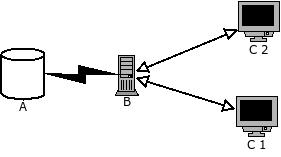
\includegraphics[scale=0.75]{wstep.jpg}
	\caption{Diagram element�w systemu}
	\end{figure}

	Obecnie w systemie ,,\loxim{}'' cz�� ,,A'' (storage) i ,,B'' (executor) s�
	zintegrowane w jednej aplikacji.
	
	Dokument ten zosta� opisany na potrzeby projektu ,,\loxim{}'', ale
	z poszanowaniem warunk�w umowy licencyjnej (GPL) protok� mo�e zosta�
	wykorzystany w dowolnej bazie danych, kt�rej potrzeby spe�nia. Rozwi�zania
	zastosowane w tym protokole wydaj� si� by� na tyle og�lne, �e z du�� pewno�ci�
	mog� zaspokoi� potrzeby wielu rozwi�za� --- tak�e relacyjnych i nie opartych o
	SBQL'a.
	
	Protok� ten stara si� po��czy� najlepsze cechy poni�szych protoko��w,
	jednocze�nie 
	skupiaj�c si� na wprowadzeniu mo�liwo�ci pracy z danymi semistrukturalnymi:
	 
	\begin{description}
	   \item[Postgresql 10] --- u�ywanego przez PostgreSQL 8.2 \cite{PostgreSQL}
	   \item[TDS 8.0] --- u�ywanego przez Sybase i Microsoft SQL Server 7.5/2000 \cite{TDS}
	   \item[MySQL 3] --- u�ywanego przez serwer MySQL 5 \cite{MySQL}
	\end{description}
	
	\subsection{Cele i za�o�enia}
	
	Celem projektu opisanego przez ten dokument jest: 
	\begin{itemize}
      \item Uzyskanie stabilnego. bezpiecznego protoko�u, umo�liwiaj�cego pe�ne
      wykorzystanie obecnych mo�liwo�ci systemu \loxim{}.
     
      \item Uzyskanie protoko�u potrafi�cego pracowa� pomi�dzy maszynami o
      r�nych architekturach sprz�towych i programowych
     
      \item Uzyskanie efektywnego (pod wzgl�dem wykorzystania sieci i CPU) 
      i �atwo rozszerzalnego protoko�u.
      
      \item Przygotowanie do implementacji sterownika JDBC w oparciu o ten
      protok�.

    \end{itemize}
    
    Przyj�to nast�puj�ce za�o�enia:
    \begin{itemize}
      \item Zak�adamy, �e komunikacja b�dzie si� odbywa�a po odpornej na
      zak��cenia, b��dy transmisji i zamian� kolejno�ci przesy�anych danych
      warstwie transportowej (TCP/IP, Unix sockets, ��cza nazwane Windows itp.).
      
      Zatem nie b�dziemy przeprowadzali w�asnej kontroli sp�jno�ci przes�anych
      danych --- pod wzgl�dem sum kontrolnych itp. Jednak ze wzgl�d�w
      bezpiecze�stwa kontrola logiczna b�dzie oczywi�cie przeprowadzana. 
    \end{itemize}
    
    \subsection{Wersjonowanie protoko�u}
    Protok� komunikacji b�dzie wersjonowany przy pomocy dw�ch numer�w:
    g��wnego (major) i pomocniczego/pobocznego (minor). Poni�szy dokument
    opisuje potok�w w wersji \wersjaproto, czyli numer g��wny \wersjaprotomajor, a pomocniczy \wersjaprotominor. Przyjmuje si�, �e aplikacje
    pos�uguj�ce si� protoko�em o tym samym numerze g��wnym s� ze sob� zgodne -
    jedynie mo�liwo�ci komunikacji s� ograniczone do tych dost�pnych w starszej
    wersji protoko�u (mniejszy numer pomocniczy). 
     
    Zatem w obr�bie tego samego numeru g��wnego mo�na przewidzie� nast�puj�ce
    typy zmian:
    \begin{itemize}
      \item[-] Rozbudowanie formatu paczki poprzez dodanie na jej ko�cu nowych
      (nie obowi�zkowych p�l).
      \item[-] Wprowadzenie nowych typ�w paczek --- niekluczowych dla
      dzia�ania systemu i niemodyfikuj�cych dotychczasowej semantyki operacji.
    \end{itemize}
    
    \subsection{Licencjonowanie}
    
    Dokument ten --- podobnie jak system \loxim{} --- jest licencjonowany na licencji
    GPL 2 (General Public License --- wersja 2). W zwi�zku z tym protok� ten mo�e
    by� wykorzystany bez dodatkowej zgody autora w dowolnym systemie
    licencjonowanym na GPL. 
    
\newpage
\section{Paczka --- jednostka logiczna komunikacji}

	\subsection{Paczka, a pakiet}
	Ca�a komunikacja b�dzie si� opiera�a o przesy�anie paczek --- sp�jnych ci�g�w
	danych o okre�lonym formacie. S�owa ,,paczka'' b�dziemy u�ywali dla rozr�nienia
	i unikni�cia nieporozumie� z poj�ciem pakietu --- kt�ry ma znaczenie na poziomie
	warstwy	transportu (np. TCP/IP).

	Zatem paczka to zbi�r danych maj�cych logiczne znaczenie w systemie \loxim{}.
	Zupe�nie nie wnikamy w to w jaki spos�b paczki zostan� zorganizowane w pakiety
	i to zadanie pozostawiamy warstwie transportu. Jedyne co musimy zagwarantowa�,
	to fakt, �e pojedyncza paczka jest sp�jnym obszarem danych w komunikacji. 
	
	W dokumencie tym b�dziemy tak�e u�ywali sformu�owania ,,komunikat'', kt�re
	uznajemy za synonim s�owa ,,paczka''. 
	
	\subsection{Budowa paczki}
		Ka�da paczka ma nast�puj�cy schemat budowy:
		\begin{bajty}
                	\bp{0}{0}{uint8}{Sta�a m�wi�ca o typie paczki, a tym samym
                	okre�laj�ca format zawartych w nich danych}
                	\bp{1}{4}{uint32}{$n$ --- sta�a okre�laj�ca
                	ilo��
                	danych w�a�ciwych zawartych w paczce -- wyra�ona w bajtach}
                	\bp{5}{$4+n$}{patrz opis zale�ny od typu paczki}{Dane w�a�ciwe paczki
                	zgodne z formatem okre�lonym poprzez typ paczki}
 		    \end{bajty}	
		Formalnie b�dziemy m�wili, �e paczka si� sk�ada z dwu-polowego nag��wka oraz
		cia�a. Nag��wek wyznacza typ paczki i rozmiar danych w�a�ciwych w niej
		zawartych, a cia�o --- to dane interpretowane zale�nie od typu paczki. Kluczow� 
		cz�� tego dokumentu stanowi opis format�w poszczeg�lnych paczek w zale�no�ci
		od ich typ�w. 
		
		Przyjmuje si�, �e rozmiar pojedynczej paczki nie mo�e przekracza� 1MB (1'048'576
		bajt�w). S�u�y to unikni�ciu sytuacji, w kt�rych odbywa si� pr�ba naruszenia
		bezpiecze�stwa serwera poprzez przes�anie zbyt du�ej paczki (doprowadzenie
		do wyst�pienia b��du OutOfMemory), a tak�e unikni�ciu sytuacji w kt�rej traci 
		si� mo�liwo�� komunikacji asynchronicznej w sko�czonym czasie (np. wys�anie do
		serwera informacji o braku dalszego zainteresowania danymi). 
		Wy�ej wymieniona sta�a mo�e by� (a nawet powinna) konfigurowalna po
		stronie serwera.
		
	\subsection{Czemu przesy�amy d�ugo�� paczki?}
		Przes�anie d�ugo�ci paczki na jej pocz�tku niesie za sob� nast�puj�ce
		u�atwienia: 
		\begin{itemize}
			\item[-] Klient mo�e zaalokowa� w�a�ciw� ilo�� danych w pami�ci operacyjnej na
			przyj�cie ca�ego komunikatu z g�ry --- co ma pozytywny wp�yw na wydajno�� i
			bezpiecze�stwo (nie nadejdzie ,,niesko�czenie'' d�ugi komunikat).
			\item[-] Klient mo�e zrezygnowa� z pobierana komunikatu (np. z powodu brak
			wystarczaj�cej ilo�ci pami�ci, by go przyj��) lub braku zainteresowania.
			Dzi�ki temu wie, ile bajt�w musi zignorowa� bez ich analizy.
        \end{itemize}
	
	\subsection{Mechanizmy rozszerzania protoko�u}
		Protok� mo�e by� rozszerzany z zachowaniem zgodno�ci wstecz poprzez
		do��czanie nowych p�l na ko�cu danych paczki. Zatem strona odczytuj�ca 
		komunikat nie mo�e zak�ada�, �e po odczytaniu wszystkich p�l w paczce o
		kt�rych wie, dotar�a na koniec paczki. Mo�liwe, �e strona ta przeczyta 
		wszystkie pola i nie dotrze wcale do ko�ca paczki, poniewa� w paczce wyst�puj�
		dane dotycz�ce nowszej wersji protoko�u. Zatem powinna ona zignorowa�
		odpowiedni� ilo�� bajt�w --- wynikaj�c� z d�ugo�ci danych w paczce, tak aby dotrze� na
		pocz�tek nast�pnego komunikatu. 
		
		Tak�e mo�liwa jest odwrotna sytuacja. Strona wysy�aj�ca pos�uguje si� starsz�
		wersj� protoko�u, wi�c wysy�a komunikat nie zawieraj�cy p�l wprowadzonych w
		nowszej wersji protoko�u. Zatem strona odczytuj�ca (kt�ra jest nowsza) powinna
		umie� w�a�ciwie zareagowa� na sytuacj�, gdy odczytano ca�� paczk�, a nie
		otrzymano nowych p�l wprowadzonych w protokole. W tej sytuacji powinna przyj��
		warto�ci domy�lne dla tych p�l. 
		
		Oczywi�cie odpowiednio du�e zmiany i przeprojektowanie w protokole mog�
		wymaga� stworzenia protoko�u o kolejnym numerze g��wnym, czyli niezgodnego ze starszymi wersjami.
	
	\newpage
\section{Podstawowe typy danych} \label{PodstawoweTypyDanych}
	
	\subsection{Postanowienia og�lne}
		\begin{itemize}
          \item Je�li w spos�b szczeg�lny nie zaznaczono inaczej (a raczej
          nigdzie nie zaznaczono) wszystkie warto�ci zapisywane s� w formacie
          \bigendian.  W szczeg�lno�ci obejmuje to typy ca�kowitoliczbowe,
          rzeczywiste, oraz napisy w kodowaniu UTF-8 tak�e stosuj� kolejno��
          \bigendian. 
        \end{itemize}               

 	 \subsection{Ca�kowitoliczbowe: uint8,  sint8, uint16, sint16, int32, uint32,
 uint64, sint64}
		
	Pierwsza litera determinuje, czy mamy do czynienia z typem ze znakiem (u -
	unsigned), czy z typem bez znaku (s --- signed).  Liczba na ko�cu wyra�a d�ugo��
	typu wyra�on� w bitach. 
	
	Typy s� kodowane oczywi�cie w kolejno�ci \bigendian. 
	
	\subsubsection{varuint --- Ca�kowitoliczbowy z kompresj� (1,3,5 lub 9 bajt�w)}
		B�dzie to typ u�ywany g��wnie do oznaczania d�ugo�ci string�w i og�lnie
		paczek. 
		
		Rozwi�zanie techniczne zosta�o zaczerpni�te z protoko�u serwera MySQL
		\cite{MySQL}.
		
		Idea jest taka, �e kr�tkie stringi ($<250$ znak�w ) b�d� si�
		pojawia�y najcz�ciej i chcemy mie� najmniejszy narzut na zapisanie d�ugo�ci
		(jedno bajtowy). 
		
		Zatem semantyka pierwszego bajtu jest nast�puj�ca (w zale�no�ci od jego
		warto�ci)
		\begin{description}
			\item[0-249] Warto�� ta jest jednocze�nie warto�ci� wynikow�
			\item[250] Warto�� jest null'em (zostawiamy dla umo�liwienia stosowanie
			tego rozwi�zania z systemami relacyjnymi) 
			\item[251] Warto�� ta poprzedza 2-bajtowe (uint16) pole w warto�ci� w�a�ciw�
			\item[252] Warto�� ta poprzedza 4-bajtowe (uint32) pole z warto�ci� w�a�ciw�
			\item[253] Warto�� ta poprzedza 8-bajtowe (uint64) pole z warto�ci�
			w�a�ciw�. Nie nale�y jednak korzysta� z warto�ci wi�kszych ni� $2^{63}-1$
			(MAX\_SINT64), ze wzgl�du na to, �e w Javie nie s� obs�ugiwane 8 bajtowe
			typy bez znaku. 
        \end{description}
		
	
	\subsection{string --- �a�cuchy tekstu}
	
	S�u�y do przesy�ania tekst�w. Teksty te musz� by� kodowane za pomoc� UTF-8. 
	
	Format warto�ci typu string jest nast�puj�cy:
	Najpierw idzie pole typu varuint --- opisuj�ce d�ugo�� w bajtach nast�puj�cego
	potem ci�gu w UTF-8 (\bigendian). 
	
	\subsection{sstring --- Kr�tki �a�cuch tekstu}
	Jest to tak naprawd� wariant typu string, 
	ale ograniczony do �a�cuch�w nie d�u�szych ni� 249 bajt�w.
	Czyli wtedy pole oznaczaj�ce d�ugo�� ma jeden bajt. 
	Jego wewn�trzna reprezentacja zupe�nie si� nie r�ni od typu
	string --- zosta� on wyr�niony formalnie --- ze wzgl�du na uproszczenie notacji 
	u�ywanej przy opisach format�w poszczeg�lnych paczek. 
	
	\subsection{bytes --- Dane binarne}
	S�u�y do przesy�ania danych binarnych (nie koniecznie du�ych --- nie b�dziemy
	tego rozr�niali na poziomie protoko�u). 
	
	Format warto�ci tego typu jest nast�puj�cy:
	Najpierw zostaje przes�ane pole typu varuint --- opisuj�ce d�ugo�� w bajtach
	nast�puj�cego potem ci�gu bajt�w.	

	\subsection{Daty i czas}
	
	\subsubsection{Kwestia stref czasowych}
	\label{strefy_czasowe}
	Mo�na rozwa�y� dwa podej�cia do przekazywania informacji o strefie czasowej:
		\begin{itemize}
          \item Przekazujemy tylko offset strefy czasowej wzgl�dem GMT (czyli
          warto�� od $-14$ do $+12$)
          \item Przekazujemy pe�n� informacj� o strefie czasowej. Wygl�da na
          to, �e nie istnieje standard ISO opisuj�cy kodowanie dla wszystkich
          stref czasowych na �wiecie. Najlepsz� baz� danych z informacjami o
          strefach czasowych jest baza TZ (znana te� jako zoneinfo)
          (http://www.twinsun.com/tz/tz-link.htm). Koduje one informacja o
          strefie czasowej w postaci napisu: \{Kontynent\}/\{Du�e miasto\} lub \{Kontynent\}/\{Pa�stwo\}/\{Du�e Miszto\}, np.
          ,,Africa/Porto-Novo''. 
          
          Zalet� przekazywania daty z t� pe�n� informacj�, jest to, �e dopiero
          na jej podstawie system informatyczny jest wstanie prawid�owo doda�
          pewn� ilo�� czasu (np. 36 godzin) do danej daty w sytuacji, gdy w
          mi�dzyczasie wyst�puje zmiana czasu z letniego na zimowy lub
          odwrotnie. 
        \end{itemize}
    
    Nie budzi w�tpliwo�ci, �e dla unikni�cia problem�w w aplikacjach o du�ym
    zasi�gu terytorialnym warto by by�o z dat� zapisywa� pe�n� informacj�.
    
    Wed�ug bazy ,,TZ'' w chwili obecnej na �wiecie jest u�ywanych 398 r�nych
    stref czasowych. Dobry standard pozwoli�by zakodowa� je za pomoc� trzech
    liter, czyli --- b�d�c rozrzutnym --- 3 bajt�w. Oszcz�dno�� 2 bajt�w wydaje si�
    by� wi�c ma�o uzasadniona wobec ryzyka utraty poprawno�ci numerycznej
    niekt�rych operacji, skoro stanowi ona wzrost d�ugo�ci ca�ej zakodowanej
    daty z 9 do 11 bajt�w, czyli o 22\%.
    
    Niestety za nieformalny standard w bazach danych (PostgreSQL, MySQL,
    Oracle, DB2) przyj�o si� zapisywa� jedynie informacje o przesuni�ciu
    wzgl�dem GMT, co wynika ze z�o�enia dw�ch problem�w:
    \begin{itemize}
      \item �wiatowy standard formatu czasu ISO8601 \cite{ISO8601} przewiduje
      tylko stref� czasow� zapisan� w postaci przesuni�cia wzgl�dem GMT. 
      \item Brak standardu (klasy ISO) kodowania stref czasowych, co po�rednio 
     wynika z punktu powy�szego.
    \end{itemize}
    
    Z tego powodu obecna wersja protoko�u zapisuje strefy czas w
    ,,standardowy'' spos�b, czyli w postaci offset�w. Zalecamy jednak 
    u�ywanie pe�nej informacji o strefie czasowej w nast�pnych wersjach
    protoko�u. 
    	
	\subsubsection{DATE}
		Sama data. 		
		
		Format nast�puj�cy:
		\begin{bajty}
	    	\bp{0}{1}{$Year$ (sint16)}{Rok}
	    	\bp{2}{2}{$Month$ (uint8)}{Miesi�c (1-stycze�, 12-grudzie�)}
	    	\bp{3}{3}{$Day$ (uint8)}{Dzie�}
    	\end{bajty}
			
	\subsubsection{TIME}
		Sam czas. 
		
		Format nast�puj�cy:
		\begin{bajty}
	    	\bp{0}{0}{$Hour$ (uint8)}{Godzina (0-23)}
	    	\bp{1}{1}{$Minuts$ (uint8)}{Minuta (0-59)}
	    	\bp{2}{2}{$Secs$ (uint8)}{Sekunda (0-59)}
	    	\bp{3}{4}{$Milis$ (sint16)}{Milisekundy (0-999)}
    	\end{bajty}
		
	\subsubsection{TIMETZ}
		Czas ze stref� czasow�
	
				Format nast�puj�cy:
		\begin{bajty}
	    	\bp{0}{0}{$Hour$ (uint8)}{Rok}
	    	\bp{1}{1}{$Minuts$ (uint8)}{Miesi�c (1-stycze�, 12-grudzie�)}
	    	\bp{2}{2}{$Secs$ (uint8)}{Dzie�}
	    	\bp{3}{4}{$Milis$ (uint16)}{Milisekundy}
	    	\bp{5}{5}{$TZ$ (sint8)}{Strefa czasowa (-14 do +12)}
    	\end{bajty}

	
		
	\subsubsection{DATETIME}
		Data i godzina bez strefy czasowej. 
		Format zapisu to bezpo�rednio po sobie wyst�puj�ce formaty p�l typu DATE i
		TIME. 


		
	\subsubsection{DATETIMETZ}
		Data i godzina ze stref� czasow�. 
		Format zapisu to bezpo�rednio po sobie wyst�puj�ce formaty p�l typu DATE i
		TIMETZ. 
			

	\subsection{Logiczne}
		Pole typu bool niesie pewn� warto�� logiczn�. W praktyce b�dzie reprezentowane
		jako liczba typu sint8 z nast�puj�cymi warto�ciami:
		\begin{description}
          \item[0]  Fa�sz
          \item[1]  Prawda
        \end{description}
	
	\subsection{Zmiennoprzecinkowe}
	   \subsubsection{DOUBLE}
	   		Podw�jna precyzja, 8-bajty w kolejno�ci \bigendian.
	
%	\subsection{Paranumeryczne}

%		Te� do ustalenia!!!	
%	\subsubsection{Numeric}
%			Jest to zapis liczby rzeczywistej przy pomocy dw�ch liczb ca�kowitych. 

\newpage	
\section{Podwarstwy}

\begin{figure}[hbt]
\centering
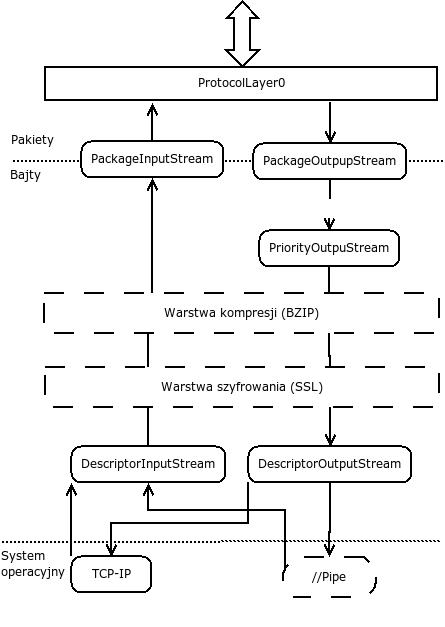
\includegraphics[scale=0.6]{warstwy.jpg}
\caption{Diagram warstw}
\end{figure}

	Protok� w warstwie aplikacyjnej mo�e chodzi� w kilku podwarstwach. Elementy te
	umo�liwiaj� szyfrowanie i kompresj� w czasie dzia�ania protoko�u.
	
	W poni�szych rozwa�aniach rozpatrzmy sytuacj� najbardziej z�o�on� --- w kt�rej
	zar�wno szyfrowania jak i kompresja jest dost�pna. 
	
	\subsection{Pisanie danych}
	
	Aplikacja chce wys�a� paczk� do innej aplikacji: 
	\begin{enumerate}
		\item	Aplikacja umieszcza (zapisuje) wysy�an� paczk� do
	strumienia wyj�ciowego. 
		\item Strumie� ten okazuje si� by� strumieniem kompresuj�cym (ZLIB), kt�ry 
		skompresowane dane zapisuje do swojego strumienia wyj�ciowego. 
		\item Strumie� ten okazuje si� by� strumieniem szyfruj�cym (SSL), kt�ry
		dokonuje szyfrowania danych, a nast�pnie umieszcza je w swoim strumieniu
		wyj�ciowym
		\item Strumie� ten okazuje si� by� strumieniem odpowiedniej warstwy
		transportu, kt�ra to warstwa przekazuje dane przez sie�.
	\end{enumerate}
	\subsection{Czytanie danych}
	
	Aplikacja chce odczyta� paczk� pochodz� od innej aplikacji. 
	\begin{enumerate}
		\item Aplikacja prosi o paczk� odpowiedni strumie� wej�ciowy.  
		\item Strumie� ten okazuje si� by� strumieniem dekompresuj�cym (ZLIB), kt�ry 
		prosi o dane sw�j strumie� wej�ciowy. 
		\item Strumie� ten okazuje si� by� strumieniem deszyfruj�cym (SSL), kt�ry
		prosi o dane sw�j strumie� wej�ciowy.
		\item Strumie� ten okazuje si� by� strumieniem odpowiedniej warstwy transportu
		i odbiera on te dane z sieci, a nast�pnie zwraca je.
		\item Strumie� deszyfruj�cy przetwarza dane i zwraca je
		\item Strumie� dekompresuj�cy przetwarza dane i zwraca je
		\item Aplikacja odczytuje dane i kompletuje je w ca�� paczk�. 
	\end{enumerate}
	
	\subsection{Inicjalizacja tych podwarstw}
		Inicjalizacja odpowiednich podwarstw odbywa si� tylko i wy��cznie w protokole
		wst�pnym. Raz zainicjalizowanych podwarstw nie mo�na wy��czy�. 

	\newpage
\section{Przep�yw komunikat�w}	

Sekcja ta opisuje przep�yw komunikat�w, a tak�e format ka�dego z komunikat�w.
W protokole mo�emy wyr�ni� kilka podprotoko��w zale�ne od stanu w kt�rym
po��czenie si� znajduje. W szczeg�lno�ci bardzo sztywno nale�y odgrodzi�
protok� wst�pny --- w kt�rym odbywa si� negocjacja parametr�w po��czenia i 
autoryzacja z protoko�em w�a�ciwym --- w kt�rym jest realizowana w�a�ciwa
funkcjonalno�ci systemu \loxim{}, a zatem wykorzystywane s� podprotoko�y:
przeprowadzania zapyta�, przesy�ania komunikatu asynchronicznego i ko�czenia
po��czenia. 

\subsection{Nazewnictwo paczek}

Na potrzeby tego dokumentu przyjmujemy nast�puj�cy schemat nazywania paczek:

	 \{znacznik grupy komunikat�w\}-\{znacznik strony, kt�ra wysy�a t�
	paczk�\}-\{identyfikator znaczenia\}
	
	Gdzie znacznik grupy paczek mo�e przyj�� nast�puj�ce warto�ci:
	\begin{description}
		\item[W] --- Podprotok� wst�pny
		\item[Q] --- Podprotok� przeprowadzania zapyta�
		\item[V] --- Podprotok� przesy�ania warto�ci
		\item[A] --- Komunikat asynchroniczny
		\item[S] --- Komunikaty standardowe (np. OK, ERROR)
    \end{description}

	Znacznikiem strony wysy�aj�cej komunikat mo�e by� jedna z nast�puj�cych
	mo�liwo�ci:
	\begin{description}
		\item[C] --- Tylko klient wysy�a tego typu komunikat
		\item[S] --- Tylko serwer wysy�a tego typu komunikat
		\item[SC] --- Zar�wno klient, jak i serwer mog� wys�a� ten komunikat
    \end{description}

\subsection{Metody opisu formatu paczki}
	Aby u�atwi� zapoznawanie si� z formatem paczek b�dziemy je prezentowali 
	w tabeli o nast�puj�cym formacie:
	\begin{bajty}
    	\bp{-5}{-5}{$\IDwcHello$ (uint8)}{Identyfikator paczki}
	    \bp{-4}{-1}{$0$ (uint32)}{D�ugo�� w�a�ciwej zawarto�ci paczki}
	    \bph
	    \bp{0}{\ldots}{warto�� (typ)}{Opis og�lny pole}	    
    \end{bajty}
		
	Nale�y zwr�ci� uwag�, �e b�dziemy prezentowali offsety wzgl�dem segmentu
	danych. 
	
\newpage
\subsection{Stany serwera} \label{diagram_stanow}

\begin{figure}[hbt]
\centering
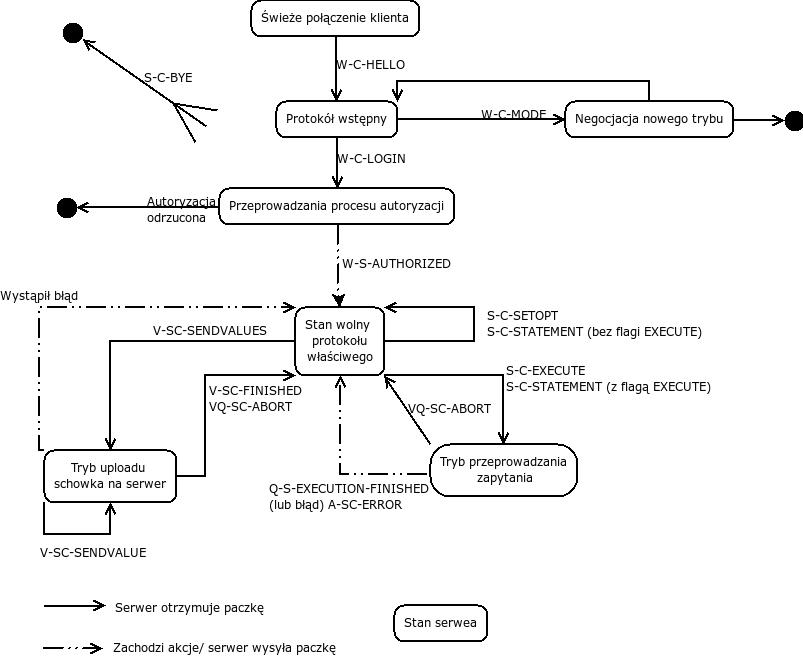
\includegraphics[scale=0.6]{stanySerwera.jpg}
\caption{Diagram przej�� i stan�w serwera}
\end{figure}

	
% \subsection{Zestawienie typ�w paczek ze wzgl�du na form� odpowiedzi}
% 
% Paczki z odpowiedzi� synchroniczn� (Odbiorca tej paczki zmuszony
% jest wys�a� odpowied� na ni� --- przed wys�aniem jakiejkolwiek innej paczki):
% \begin{description}
% 	\item[]
% 	\item[\ldots lista nie kompletna !!!]
% \end{description}
% 
% Paczki bez odpowiedzi: 
% \begin{description}
% 	\item[]
% 	\item[\ldots lista nie kompletna !!!]
% \end{description}

\subsection{Protok� wst�pny}
	Protok� wst�pny s�u�y do negocjacji parametr�w po��czenia
	(kto, do kt�rej bazy danych, czy z szyfrowaniem i kompresj�, jakie s�
	mo�liwo�ci serwera i klienta), a tak�e do przeprowadzenia autoryzacji
	u�ytkownika. 	
	
	Og�lny schemat konwersacji jest nast�puj�cy:
	\begin{enumerate}
      \item Klient nawi�zuje po��czenie (w przypadku TCP otwiera odpowiedni port
      na odpowiednim komputerze)
      \item Serwer (o ile nie jest skonfigurowana polityka odrzucania po��cze� z
      hosta klienta - raczej na zaporze sieciowej) przyjmuje (akceptuje) po��czenie i nic nie wysy�a.
      \item Klient wysy�a paczk� \pac{W-C-HELLO} --- klient ujawnia, �e chce
      rozmawia� z \loxim{}'em po tym protokole. 
      \item Serwer odpowiada paczk� \pac{W-S-HELLO} --- serwer ujawnia swoje cechy
      i mo�liwo�ci. 
   
      \item Klient ewentualnie (kilkukrotnie) wysy�a paczk� \pac{W-C-MODE} --- w kt�rym prosi
      serwer o zmian� trybu (w��czenie kompresji, szyfrowania). 
      Odbywa si� stosowna konwersacja zwi�zana z zam�wionymi podwarstwami (je�li
      serwer je obs�uguje --- np. SSL handshake). Serwer potwierdza przyj�cie zlecenia
		wykonania tej 
      operacji \pac{S-SC-OK} lub zg�asza b��d \pac{S-SC-ERROR}. Nast�pnie mo�e 
      zosta�
      przes�any zestaw paczek negocjuj�cych nowy tryb.  Nast�pny komunikat
      jest transportowany ju� w nowym trybie. 
      
      \item Klient ewentualnie ustala po��dane cechy po��czenia \pac{S-C-SETOPT}
      \item Serwer potwierdza, b�d� odrzuca ich przyj�cie. 
      
      \item Klient wybiera protok� logowania i informuje o nim serwer
      \pac{W-C-LOGIN}. Serwer przeprowadza konwersacj� autoryzuj�c� z klientem
      wed�ug jednej z metod. Podstawowe metody autentykacji opisane s� w
      dalszej cz�ci tego dokumentu \patrz{metodyAutoryzacji}.
      
      \item Ostatecznie serwer b�d� informuje klienta o zatwierdzeniu
      autoryzacji \pac{W-S-AUTHORIZED} b�d� odrzuca j� i
      zamyka po��czenie \pac{S-SC-ERROR}.
      \item Protok� wst�pny zostaje zako�czony. 
    \end{enumerate}
    
    %%%Tu wstawi� schemat UML tej konwersacji
 	\newpage
	\subsubsection{W-C-HELLO} \label{W-C-HELLO}
	Paczka s�u�y nawi�zaniu w�a�ciwego po��czenia na poziomie logicznym pomi�dzy
	klientem, a serwerem. Stanowi form� przedstawienia, dzi�ki kt�rej serwer nabywa
	przekonanie, �e ma do czynienia z uczciwym klientem, a nie skanerem port�w, a 
	tak�e przedstawia serwerowi dane, kt�re mog� by� przydatne --- g��wnie do cel�w
	administracyjnych (�ledzenie stanu serwera, diagnostyka).
	
	Mo�na wyr�ni� nast�puj�ce grupy p�l w tym komunikacie
	\begin{description}
      \item[Cechy procesu klienta: PID, nazwa, wersja, hostname] 

		S�u�� one umo�liwieniu �ledzenia akcji maj�cych miejsce 
		aktualnie na serwerze oraz sporz�dzanie statystyk i log�w dotycz�cych
		aktywno�ci pojedynczej aplikacji klienta lub pojedynczej maszyny klienckiej.
		Podawanie PIDu i hostname'a umo�liwia np. administratorowi zatrzymanie
		konkretnego procesu, kt�ry obci��a zbytnio serwer. 
		
		Oczywi�cie --- jak zawsze, ale tu szczeg�lnie --- w �aden spos�b nie nale�y
		informacjom podawanym tutaj ufa�. Zatem np. decyzj� o 'dost�pnych' metodach
		logowania serwer powinien podejmowa� na podstawie adresu IP pobranego z danych
		po��czenia --- a nie na podstawie hostname'a przes�anego w tym pakiecie. 
		
      \item[Cechy regionalne: Strefa czasowa]
		Strefa czasowa b�dzie domy�ln� stref� w kt�rej serwer b�dzie podawa� i
		przyjmowa� godziny i daty (gdy s� one pozbawione informacji o strefie, kt�rej dotycz�).
		
		W tym przypadku ponownie (z konieczno�ci --- \patrz{strefy_czasowe}) pos�ugujemy
		si� stref� czasow� zapisan� w postaci r�nicy czasu mi�dzy czasem lokalnym, a czasem GMT. 
		
      \item[Cechy regionalne: Por�wnywanie napis�w (collation)]
		Pole ,,collation'' s�u�y przekazaniu informacji o obowi�zuj�cej metodzie
		por�wnywania napis�w. W obecnej wersji systemu \loxim{} pole to nie b�dzie wykorzystywane, ale
		ju� zapewniamy na jago potrzeby 64bity (np. pierwsze 32 bity mog� pos�u�y� do
		okre�lenia j�zyka, kt�ry stosujemy, a drugie 32 bity mog� by� wykorzystywane
		na flagi (np. czy $A>a$, czy mo�e $A=a$)). W szczeg�lno�ci przekazuj�c te
		dane (j�zyk i zestaw flag) do algorytmu ,,Unicode Technical Standard \#10,
		Unicode Collation Algorithm'' \cite{UTS10}, mo�na otrzyma� zasady
		por�wnywania napis�w odpowiednie dla wybranego j�zyka.  
		
		Z algorytmu UTS wynika, �e drugie 32 bity mo�na wykorzysta� w nast�puj�cy
		spos�b do jego parametryzowania (podajemy numery najmniej znacz�cych bit�w od
		0 do 31:
		\begin{description} 
			\item[0-3] --- Te 4 bity wykorzystujemy do przechowania w�asno�ci ,,Level'',
			czyli liczby cech uwzgl�dnianych przy sortowaniu. UTS przewiduje nast�puj�ce
			5 poziom�w:  
			 \begin{description}
			   \item[0] --- zasada domy�lna dla j�zyka
               \item[1] --- L1 (Base letters)
               \item[2] --- L2 (L1+Accents)
               \item[3] --- L3 (L2+Case)
               \item[4]	 --- L4 (L3+Punct)
               \item[5] --- L5 (L4+Codepoint)
             \end{description}
			\item[4-5] --- Te dwa bity wykorzystamy do przechowania zachowania wzgl�dem
			por�wnywania znak�w wielkich i ma�ych. Proponujemy by:
			\begin{description}
				\item[0] --- Nie wymuszaj (domy�lnie dla j�zyka)
				\item[1] --- Uznawaj wielkie i ma�e litery za to�same
				\item[2] --- Wielkie litery pierwsze 	
				\item[3] --- Ma�e litery pierwsze	
			\end{description}	
			\item[6] Je�li bit zapalony, to u�ywamy opcji ,,French accents''
			\item[7] Je�li bit zapalony, to u�ywamy opcji ,,Add case Level''
			\item[8] Je�li bit zapalony, to u�ywamy opcji ,,Full normalization mode''
			\item[9] Je�li bit zapalony, to u�ywamy opcji ,,Add Hiragana Level''
			\item[10] Je�li bit zapalony, to u�ywamy opcji ,,Numeric Collation''
			\item[11-31] aktualnie nie u�ywane 	
		\end{description}	 
		
      \item[Cechy regionalne: J�zyk klienta]
		J�zyk klienta s�u�y tylko umo�liwieniu przesy�ania komunikat�w (takich jak
		komunikaty o b��dach) w j�zyku mo�liwie bliskim j�zykowi u�ytkownika. Je�li
		j�zyk wybrany t� opcj� nie jest wspierany, to system wybiera inny --- mo�liwie
		bliski wybranemu lub domy�lny (np. angielski).
		
		Kodowanie znak�w nie jest przesy�ane --- ze wzgl�du na za�o�enie, �e
		wszelka komunikacja tekstowa b�dzie prowadzona za pomoc� kodowania UTF-8
		(\bigendian). Zatem zawsze do klienta nale�y przekodowanie takiego napisu z i
		na stron� kodow� klienta. 
    \end{description}

		G��bszych rozwa�a� na poziomie implementacji serwera bazy danych wymaga
	kwestia traktowania danych regionalnych takich jak strefa czasowa, czy metoda
	por�wnywania napis�w.
	 
	Niekt�re serwery baz danych dokonuj� w r�ny spos�b konwersji danych
	zawartych w bazie danych na czas lokalny ``sesji'' u�ytkownika. Protok�
	zaleca, by takie zachowanie podlega�o konfiguracji za pomoc� opcji obs�ugiwanych 
	przez pakiet \pac{S-C-SETOPT}.
	
	Podobn� kwesti� jest to, na jakim poziomie baza danych powinna pami�ta� metod�
	por�wnywania napis�w. Relacyjne bazy danych takie jak MySQL i MSSQL pami�taj� j� na
	poziomie kolumny w tabeli), co jest do�� elastycznym rozwi�zaniem (cho� czasem
	zaskakuje programist�, gdy odkrywa, �e przeszukiwania po jednej kolumnie s�
	czu�e na wielko�� znak�w, a po drugiej kolumnie w tej samej tabeli nie s�).
	Wyst�puj�cym, ale uzasadnionym problemem w tym rozwi�zaniu jest to, �e
	nie mo�na por�wnywa� warto�ci w dw�ch kolumnach o r�nych metodach
	por�wnywaniu napis�w (w tej sytuacji wzorowa baza danych powinna udost�pni�
	mechanizm specyfikacji wed�ug kt�rej kolacji to por�wnanie ma dzia�a� --- z czym
	w praktyce si� jeszcze nie spotka�em). 
	
	Brak schematu w modelu $AS_0$ bazy Loxim uniemo�liwia takie zapami�tywanie
	informacji o ,,collation''. Zapami�tywanie tej informacji z ka�dym napisem
	wydaje si� by� skrajnie niepraktyczne (du�y koszt pami�ciowy i niska potencjalna
	u�yteczno��). Za podporz�dkowaniem metody por�wnywania napis�w do
	ustawie� sesji przemawia sytuacja, gdy u�ytkownik przyzwyczajony do j�zyka
	np. szwedzkiego prosi baz� danych o przygotowaniu mu posortowanej listy
	jego mi�dzynarodowych kontrahent�w i oczekuje, �e dostanie t� baz� posortowan�
	wed�ug wytycznych jego j�zyka. Z analogicznym roszczeniem do tej bazy mo�e
	wyst�pi� Niemiec --- dla kt�rego naturalne zasady sortowania s� nieco inne.
	Dlatego w zale�no�ci od ustawienia aplikacji klienckiej (a zatem sesji)
	powinna by� wybrana metoda por�wnywania napis�w.
	
	Z drugiej strony --- nie jest rzecz� w�a�ciw�, gdy zapytanie
	(Emp where title='Programmer') da nam r�ne wyniki w zale�no�ci od ustawie� naszej
	aplikacji klienckiej (np. w jednym przypadku z uwzgl�dnieniem wielko�ci
	znak�w, a w drugim bez uwzgl�dnienia wielko�ci znak�w). Pewnym rozwi�zaniem w
	tym przypadku jest specyfikowanie metody na poziomie np. korzeni (root�w). 
	
	Protok� nie specyfikuje, kt�re rozwi�zanie jest s�uszne, ale udost�pnia pole,
	kt�re mo�e by� wykorzystane do przes�ania tych danych. Tak�e przy zastosowaniu zar�wno jednego jak i drugiego rozwi�zania
	pole to mo�e by� �r�d�em danych dla odpowiedniej konfiguracji nowo tworzonych obiekt�w. 
			
	Format pakietu W-C-Hello jest nast�puj�cy:
	\begin{bajty}
    	\bp{-5}{-5}{$\IDwcHello$ (uint8)}{Identyfikator paczki}
	    \bp{-4}{-1}{$a$ (uint32)}{D�ugo�� w�a�ciwej zawarto�ci paczki}
	    \bph
	    \bp{0}{7}{sint64}{PID procesu klienta --- mo�e by� 0, gdy nie obs�ugiwany}
	    \bp{8}{k}{sstring}{Nazwa programu klienckiego.}
	    \bp{$k+1$}{$l$}{sstring}{Wersja programu klienckiego.} 
  	    \bp{$l+1$}{$m$}{sstring}{Hostname --- nazwa komputera (z domen�).}
   	    \bp{$m+1$}{$m+3$}{sstring (3 znaki)}{J�zyk u�ytkownika --- kod literowy wed�ug
   	    standardu ISO-639-2 (http://www.loc.gov/standards/iso639-2/php/code\_list.php)} 
		\bp{$m+4$}{$m+11$}{uint64}{Kolacji }		%!!! --- doprecyzowa�
	    \bp{$m+12$}{$m+12$}{sint8}{Strefa czasowa klienta w postaci liczby
	    ca�kowitej opisuj�cej przesuni�cie wzgl�dem GMT. Czyli dopuszczalne 
	    warto�ci to od -14 (to nie jest b��d) do +12. } 
    \end{bajty}
	
	\newpage
	\subsubsection{W-S-HELLO} \label{W-S-HELLO}
	Paczka s�u�y przedstawieniu mo�liwo�ci protoko�u i podstawowych informacji o
	serwerze. 
	
	Zatem jego format jest nast�puj�cy:
	\begin{bajty}
    	\bp{-5}{-5}{$\IDwsHello$ (uint8)}{Identyfikator paczki}
	    \bp{-4}{-1}{$a$ (uint32)}{D�ugo�� w�a�ciwej zawarto�ci paczki}
	    \bph
	    \bp{0}{0}{p\_major=\wersjaprotomajor (uint8)}{Numer g��wny (major) wersji protoko�u}
	    \bp{1}{1}{p\_minor=\wersjaprotominor (uint8)}{Numer pomocniczy (minor)
	    wersji protoko�u}  
	    \bp{2}{2}{s\_major (uint8)}{Numer g��wny (major) wersji systemu}
	    \bp{3}{3}{s\_minor (uint8)}{Numer pomocniczy (minor) wersji systemu}  	    
	    \bp{4}{7}{max\_package\_size (uint32)}{Rozmiar maksymalnego paczki 
	    przesy�anego tym protoko�em --- powinno by� $>1024$ i warto�� powy�ej  $1048586$ powinna by� istotnie uzasadniona (warto�� jest odczytywana z    konfiguracji serwera)}
	    \bp{8}{15}{features (uint64)}{Mapa bitowa dost�pnych cech serwer'a}
	    \bp{16}{23}{auth\_methods (uint64)}{Mapa bitowa dost�pnych metod
	    autoryzacji} 
	    \bp{24}{43}{salt (char[20])}{160 bitowy ci�g losowy --- u�ywany przez
	    niekt�re metody autoryzacji}
    \end{bajty}

	Dost�pne features dziel� si� na: 
	\begin{description}
		\item[Tryby transmisji i dzia�ania protoko�u:]\label{TrybyTransmisji}
		\begin{description}
			\item[0x0001=F\_SSL]  --- po��czenie mo�e by� szyfrowane metod� SSL
	 		\item[0x0002=F\_O\_SSL]  --- obligatoryjne po��czenie szyfrowane metod� SSL
		(wymusza te� obecno�� flagi F\_SSL)
			\item[0x0004=F\_ZLIB] --- po��czenie mo�e by� kompresowane za pomoc� biblioteki
		ZLIB 
		\end{description}

		\item[Tryb przetwarzania zapytania:]		
		\begin{description}
			 \item[0x0010=F\_AUTOCOMMIT] --- serwer udost�pnia tryb autocommit (ka�de
		zapytanie zadane poza transakcj� rozpoczyna swoj� transakcj�, kt�re jest
		automatycznie zamykana po wykonaniu polecenia)
			\item[0x0020=F\_OPTIMALIZATION] --- mo�na w��czy� optymalizator zapyta�
			\item[\ldots np. poziomy izolacji transakcji] 
	    \end{description}
    \end{description}

	\label{MetodyAutoryzacji}
	Aktualnie przewidziane metody autentykacji to auth\_methods to:
	\patrz{metodyAutoryzacji}
	\begin{description}
		\item[0x0001=AM\_TRUST] --- serwer uwierzy w ka�d� podan� to�samo��
		(\patrz{authTrust})
		\item[0x0002=AM\_MYSQL5\_AUTH] --- autoryzacja metod� stosowan� przez serwer
		(\patrz{authMySQL}) MySQL5 \cite{MySQL} --- w oparciu o przesy�anie i
		przechowywanie skr�tu has�a algorytmem SHA1. 
		Generalnie schemat jest nast�puj�cy:
		\begin{description}
			\item[Serwer przechowuje:] $SHA1(password)$
			\item[Klient przesy�a:] $SHA1(password) XOR (SHA1(salt.SHA1(SHA1(password))))$
	    \end{description}
	\end{description}
	
	\subsubsection{W-C-MODE} \label{W-C-MODE}
	Jest to paczka s�u��ca do przej�cia w protokole wst�pnym na inny tryb
	transmisji. Obecnie obejmuje to koncepcj� szyfrowania, kompresji, a tak�e
	ewentualnie transmisji w formacie XML.
	
	Jedynym parametrem paczki jest wybrany tryb transmisji. Zatem format paczki
	jest nast�puj�cy:
	\begin{bajty}
    	\bp{-5}{-5}{$\IDwcMode$ (uint8)}{Identyfikator tej paczki}
	    \bp{-4}{-1}{$8$ (uint32)}{D�ugo�� w�a�ciwej zawarto�ci paczki}	    
	    \bph{}
	    \bp{0}{7}{nowy\_tryb (uint64)}{JEDNA ze sta�ych trybu transmisji: }		
    \end{bajty}

	Przewidywane tryby transmisji to:
	\begin{description}
    	\item[TT\_SSL=1]  komunikacja szyfrowana z wykorzystaniem protoko�u SSL
    	\item[TT\_ZLIB=2] komunikacja kompresowana
    \end{description}
	
	W kolejne tryby nale�y wchodzi� pojedynczo. Nowy tryb umieszczany jest na
	szczycie stosu (warstwa transportu znajduje si� na spodzie stosu). Zatem, aby
	sensownie uruchomi� jednocze�nie kompresj� i szyfrowa�, nale�y najpierw uruchomi�
	szyfrowanie, a p�niej kompresj�. W ten spos�b dane zostan� najpierw
	skompresowane, a p�niej zaszyfrowane. 

	Dost�pne odpowiedzi to:
	\begin{description}
		\item[S-SC-OK]	Polecenie zosta�o zaakceptowane. Za chwile nast�pi� negocjacje
		w kwestii ustalenia nowego trybu. Szczeg�y ustalenia konkretnego trybu zale��
		od wybranego trybu. Strona, kt�ra inicjalizuje dalsza konwersacj� tak�e zale�y od konkretnego elementu (np.
	 	w przypadku SSL'u serwer powinien rozpocz�� ,,HANDSHAKE''). 

		Je�li proces negocjacji nowego trybu zako�czy si� pora�k�, to po��czenie
		musi zosta� natychmiast zerwane. 

		\item[S-SC-ERROR]  Nie jest mo�liwe przej�cie to ��danego trybu z jakiego�
		powodu. Spodziewane komunikaty odpowiedzi to mo�e by�:
		\begin{description}
			\itemERR{ModeNotAvoilable}
			\itemERR{ModeAlredySet}
			\itemERR{Internal}
		\end{description}			

	\end{description}

	
			
	\subsubsection{W-C-LOGIN} \label{W-C-LOGIN}
	Komunikat s�u�y przekazaniu przez klienta serwerowi informacji
	o tym, za pomoc� kt�rego mechanizmu logowania klient b�dzie si� chcia�
	zalogowa� do serwera. 
	W praktyce jedynym parametrem paczki jest identyfikator wybranej metody autoryzacji
	\ref{metodyAutoryzacji}). Zatem format paczki jest nast�puj�cy:	
	\begin{bajty}
    	\bp{-5}{-5}{$\IDwcLogin$ (uint8)}{Identyfikator paczki login}
	    \bp{-4}{-1}{$8$ (uint32)}{D�ugo�� w�a�ciwej zawarto�ci paczki}	    
	    \bph{}
	    \bp{0}{7}{nowy\_tryb (uint64)}{JEDNA z warto�ci metody autoryzacji (patrz: 
	    \ref{metodyAutoryzacji})}		
    \end{bajty}
	
	W momencie wys�ania tej paczki --- zarz�dzanie protoko�em jest oddane procesowi
	realizuj�cemu konkretn� metod� autoryzacji. Metoda taka powinna zapewni� to,
	�e serwer po jej realizacji wy�le pakiet W-S-AUTHORIZED lub zg�osi b��d i
	zako�czy po��czenia, a klient po zako�czeniu dzia�anie tej metody, b�dzie
	wiedzia�, �e ona si� zako�czy�a i b�dzie gotowy na odbi�r pakietu
	W-S-AUTHORIZED lub informacji o b��dzie.
	
	W sytuacji, gdy serwer otrzyma paczk� W-C-LOGIN chc�c� przeprowadzi�
	autoryzacj� metod� nie wspieran� przez serwer --- serwer powinien natychmiast
	zerwa� po��czenie. 
	
	\subsubsection{W-S-AUTHORIZED} \label{W-S-AUTHORIZED}
	Jest to paczka potwierdzaj�ca skuteczn� autoryzacje i o�wiadczaj�cy o
	zako�czeniu pracy serwera w trybie wst�pnym i o m�wi�cy przej�ciu w tryb
	pracy w�a�ciwej. 
	
	Format jest nast�puj�cy:
	\begin{bajty}
    	\bp{-5}{-5}{$\IDwsAuthirized$ (uint8)}{Identyfikator tej paczki}
	    \bp{-4}{-1}{$0$ (uint32)}{D�ugo�� w�a�ciwej zawarto�ci paczki}	    
    \end{bajty}

	\subsubsection{W-C-PASSWORD} \label{W-C-PASSWORD}
	Jest to paczka w kt�rym klient autoryzuj�cy si� przy pomocy has�a powinien
	przes�a� sw�j login i has�o. W szczeg�lno�ci ta paczka wykorzystuje metody
	autoryzacji: Trust oraz MySQLpassword \patrz{metodyAutoryzacji}. 
	
	Format jego jest nast�puj�cy:
	\begin{bajty}
    	\bp{$-5$}{$-5$}{$\IDwcPassword$ (uint8)}{Identyfikator tej paczki}
	    \bp{$-4$}{$-1$}{$m$ (uint32)}{D�ugo�� w�a�ciwej zawarto�ci tego 
	    paczki}	    
	    \bph{}
	    \bp{$0$}{$n$}{login (sstring)}{Login autoryzuj�cego si� u�ytkownika}
	    \bp{$n+1$}{$m-1$}{password (bytes)}{Has�o lub jego skr�t lub NULL w
	    przypadku metody Trust}
    \end{bajty}

\subsection{Protok� w�a�ciwy --- obs�uga zapytania}\label{proto_obsluga_zapytan}
	
	\subsubsection{Q-C-STATEMENT} \label{Q-C-STATEMENT}
		Paczka s�u�y do przes�ania zapytania na serwer. Je�eli flaga EXECUTE jest
		zapalona --- to znaczy, �e przesy�amy proste --- bezparametrowe zapytanie --- kt�re
		chcemy by zosta�o natychmiast wykonane przez serwer. W przeciwnym przypadku
		przesy�amy tylko zapytanie --- by zosta�o sparsowany --- i by zosta� my nadany
		numer StetementId. Pos�uguj�c si� p�niej tym numerem b�dziemy mogli
		wielokrotnie zbindowa� parametry do zapytania i je wykona� (\pac{Q-C-EXECUTE}). 
		
		Format paczki jest nast�puj�cy:
		\begin{bajty}
	    	\bp{$-5$}{$-5$}{$\IDqcStatement$ (uint8)}{Identyfikator tej paczki}
		    \bp{$-4$}{$-1$}{$m$ (uint32)}{D�ugo�� w�a�ciwej zawarto�ci tej paczki}	    
		    \bph{}
		    \bp{$0$}{$7$}{flags (uint64)}{Flagi ustawiaj�ce opcje zapytania (patrz:
		    dost�pne flagi poni�ej)}
		    \bp{$8$}{$m-1$}{statement (string)}{Zapytanie wysy�ane na serwer}
		 \end{bajty}

		Aktualnie przewidziane flagi to:
		\begin{description}
			\item[EXECUTE = 0x0001]  --- je�li flaga jest zapalona to zapytanie zachowuje
			si� tak, jakby natychmiast po nim zosta�a wys�ana \pac{Q-C-EXECUTE}. Czyli
			zamiast odpowiedzi \pac{Q-S-STMTPARSED} pojawi si� albo odpowied�
			\pac{Q-S-EXECUTING}, albo zostanie zg�oszony kt�ry� z b��d�w charakterystycznych dla polece�
			\pac{Q-C-STATEMENT} i \pac{Q-C-EXECUTE}. 
			
			\item[READONLY = 0x0002] --- je�li flaga jest zapalona to zapytanie nie ma
			prawa wprowadza� �adnych modyfikacji w bazie danych  
        \end{description}

		W odpowiedzi na t� paczk� mo�e przyj�� paczka \pac{Q-S-STMTPARSED} (je�li nie
		by�a
		podniesiona flaga EXECUTE) albo (\pac{Q-S-EXECUTING} --- je�li by�a podniesiona
		flaga EXECUTE) albo jeden z poni�szych b��d�w:
		\begin{description}
			\itemERR{SyntaxError}
			\itemERR{OperationNotAllowed}
			\itemERR{Internal}
			\item[oraz b��dy charakterystyczne dla \pac{Q-C-EXECUTE}] --- o ile flaga
			EXECUTE jest zapalona
        \end{description}
		
	\subsubsection{Q-S-STMTPARSED} \label{Q-S-STMTPARSED}
		Paczka informuje, �e analiza sk�adniowa zapytania si� powiod�a i, �e zapytaniu
		zosta� nadany StatementId. Paczka jest wysy�ana w spos�b synchroniczny w
		odpowiedzi na komunikat \pac{Q-C-STATEMENT}. 
		
		Format jest nast�puj�cy:
		\begin{bajty}
	    	\bp{$-5$}{$-5$}{$\IDqcStmtparsed$ (uint8)}{Identyfikator tej paczki}
		    \bp{$-4$}{$-1$}{$16$ (uint32)}{D�ugo�� w�a�ciwej zawarto�ci tej paczki}	    
		    \bph{}
		    \bp{$0$}{$7$}{statementId (uint64)}{Id nadane temu zapytaniu/poleceniu}
		    \bp{$8$}{$15$}{paramsCnt  (uint32)}{Liczba parametr�w do ustalenia w
		    sparsowanym zapytaniu. }
		 \end{bajty}	
	
	\subsubsection{Q-C-EXECUTE}  \label{Q-C-EXECUTE}
		Paczk� t� wysy�a klient w celu poinformowania serwera o tym, �e chce wykona�
		zadane poprzez statementId zapytanie. Cz�sto, tak�e tym zapytaniem b�dzie si�
		dokonywa�o bindowania bindowania poszczeg�lnych parametr�w zapytania z
		identyfikatorami warto�ci w schowku (patrz obs�uga schowka) w celu wykonania
		zapytania. 
		
		Format paczki jest nast�puj�cy:
		\begin{bajty}
	    	\bp{$-5$}{$-5$}{$\IDqcExecute$ (uint8)}{Identyfikator tej paczki}
		    \bp{$-4$}{$-1$}{$m$ (uint32)}{D�ugo�� w�a�ciwej zawarto�ci tej paczki}	    
		    \bph{}
		    \bp{$0$}{$7$}{statementId (uint64)}{Id nadane temu zapytaniu/poleceniu}
		    \bp{$8$}{$15$}{flags (uint32)}{Flagi --- wskaz�wki dotycz�ce wynik�w
		    zapytania --- patrz ni�ej}
		    \bp{$16$}{$19$}{paramsCnt  (uint32)}{Liczba parametr�w do ustalenia w
		    sparsowanym zapytaniu. }		    
		    \bp{$m_{i-1}$}{$m_{i}-1$}{$valueId_i$  dla $i \in (1..paramsCnt)$
		    (varuint)}{Id b�d�ce i-tym parametrem. Id powinno si� odnosi� do Id 
		    warto�ci znajduj�cym si� w schowku sesji --- ustalonym uprzednio poprzez
		    paczk� \pac{V-SC-SENDVALUE}}			       
		 \end{bajty}	

		Przewidywane flagi to (ci�g dalszy do flag z Q-C-STATEMENT):
		\begin{description}
			\item[0x0100 PREFER-DFS] Oznacza, �e u�ytkownik sugeruje by wyniki by�y
			przesy�ane w kolejno�ci umo�liwiaj�cej szybk� konstrukcj� odpowiedzi metod�
			DFS. Wyklucza si� z PREFER-BFS.
			
			\item[0x0100 PREFER-BSF] Oznacza, �e u�ytkownik sugeruje by wyniki by�y
			przesy�ane w kolejno�ci umo�liwiaj�cej szybk� konstrukcj� odpowiedzi metod�
			BFS. Wyklucza si� z PREFER-DFS.
        \end{description}

		Paczka w spos�b synchroniczny jest zwi�zana z odpowiedzi� \pac{Q-S-EXECUTING}
		lub jednym z nast�puj�cych b��d�w:
		\begin{description}
			\itemERR{ParamsIncomplete}
			\itemERR{NoSuchValueId}
			\itemERR{OperationNotPermited}
			\itemERR{Internal}
        \end{description}
			
	\subsubsection{Q-S-EXECUTING} \label{Q-S-EXECUTING}
 		Paczka ta jest synchronicznym powiadomieniem o przyj�ciu do przetworzenia
 		danego zapytanie (czyli jest wysy�ana w odpowiedzi na pakiety
 		\pac{Q-C-EXECUTE} oraz \pac{Q-C-STATEMENT} (z flag� EXECUTE)).
 		
 		Format pakietu jest nast�puj�cy:
 		\begin{bajty}
     		\bp{-5}{-5}{$\IDqsExecuting$ (uint8)}{Identyfikator paczki EXECUTING}
 	    	\bp{-4}{-1}{$0$ (uint32)}{D�ugo�� w�a�ciwej zawarto�ci paczki}
     	\end{bajty}
 
 		Otrzymanie tej paczki �wiadczy o tym, �e klient znalaz� si� w trybie
 		wykonywania zapytania (tzn. �e nie mo�emy wys�a� nowego zapytania do czasu
 		przetworzenia lub anulowania bie��cego zapytania, a tak�e to, �e 
 		aktualnie otrzymywane pakiety z grupy V-\ldots dotycz�ce wynik�w zwracanych
 		przez to zapytanie).
			
		
% 	\subsubsection{Q-C-CANCEL} \label{Q-C-CANCEL}
% 		Paczka ta jest ��daniem przerwania przetwarzania bie��cego zapytania. Po jej
% 		otrzymaniu serwer ma obowi�zek przesta� wylicza� zapytanie, a nast�pnie
% 		opr�ni� kolejk� pakiet�w wychodz�cych z wszystkich pakiet�w zwi�zanych z tym
% 		zapytaniem (a wi�c tak�e paczki z grypy V-xx-xxx), a nast�pnie wys�a� w synchroniczny
% 		
% 		Format pakietu jest nast�puj�cy:
% 		\begin{bajty}
%    		\bp{-5}{-5}{$\IDqcCancel$ (uint8)}{Identyfikator paczki Cancel}
%     	\bp{-4}{-1}{$0$ (uint32)}{D�ugo�� w�a�ciwej zawarto�ci paczki}
% 	   \end{bajty}
% 
% 		B��dy kt�re mog� pojawi� si� w odpowiedzi na ten pakiet to:
% 		\begin{description}
% 			\itemERR{NoCurrentStatement}
% 			\itemERR{Internal}
%       \end{description}
% 		Po otrzymaniu odpowiedzi \pac{S-SC-OK} znajdujemy si� poza trybem wykonywania zapytania -
% 		wi�c mo�emy wykona� nast�pne. 
% 		
% 		W sytuacji wyst�pienia b��du nale�y przyj��, �e znajdujemy si� poza trybem
% 		wykonywania zapyta�, a w przypadku b��du internal najbezpieczniej roz��czy�
% 		po��czenie i nawi�za� ��czno�� ponownie. 
		
% 	\subsubsection{Q-S-NORESULT} \label{Q-S-NORESULT}
% 		Paczka informuje, �e bie��ce zapytanie si� zako�czy�o i nie zwr�ci�o �adnych
% 		wynik�w --- mimo, �e by�o zapytaniem (a nie aktualizacj� danych). 	
% 	
% 		Format paczki jest nast�puj�cy:
% 		\begin{bajty}
%     		\bp{-5}{-5}{$\IDqsNoResult$ (uint8)}{Identyfikator paczki No-result}
% 	    	\bp{-4}{-1}{$0$ (uint32)}{D�ugo�� w�a�ciwej zawarto�ci paczki}
%     	\end{bajty}
% 
% 		Wys�anie (ale nie umieszczenie w kolejce pakiet�w do wys�ania) tej paczki przez
% 		serwer powoduje, �e przechodzi on w tryb nie przetwarzania zapytania. 
% 		
	\subsubsection{Q-S-EXECUTION-FINISHED} \label{Q-S-EXECUTION-FINISHED}
		Paczka informuje, �e bie��ce polecenie si� zako�czy�o i ewentualnie informuje
		o liczbie zmian dokonanych przez to zadanie.  
	
		\hyphenation{mod-Atom-Po-inter-Cnt}
		Format pakietu jest nast�puj�cy:
		\begin{bajty}
    		\bp{$-5$}{$-5$}{$\IDqsOperationOk$ (uint8)}{Identyfikator paczki operationOk}
	    	\bp{$-4$}{$-1$}{$a$ (uint32)}{D�ugo�� w�a�ciwej zawarto�ci paczki}
	    	\bph
	    	\bp{$0$}{$d-1$}{modAtomPointerCnt (varuint)}{ liczba zmodyfikowanych obiekt�w
	    	atomowych i pointerowych przez to zdanie (je�li nie jest okre�lona to serwer ma
	    	to zwr�ci� NULL)}
	    	\bp{$d$}{$b-1$}{delCnt (varuint)}{liczba usuni�tych obiekt�w (je�li nie jest okre�lona to serwer ma to zwr�ci� NULL)}
	    	\bp{$b-1$}{$c$}{newRootsCnt (varuint)}{liczba utworzonych obiekt�w korzeniowych (je�li nie jest okre�lona to serwer ma to zwr�ci� NULL)}
	    	\bp{$c-1$}{$a-1$}{insertsCnt (varuint)}{liczba obiekt�w wstawionych do obiekt�w z�o�onych (r�wnie� tych
nowo utworzonych) (je�li nie jest okre�lona to serwer ma to zwr�ci� NULL)}
    	\end{bajty}

		Wys�anie (ale nie umieszczenie w kolejce paczek do wys�ania) tej paczki przez
		serwer powoduje, �e wychodzi on z trybu przetwarzania zapytania.  
		
		Wysy�anie ilo�ci dokonanych zmian ma u�atwi� prac� system�w korzystaj�cych z
		mechanizmu tzw. optymistycznego przetwarzania transakcji przez aplikacj�
		klienck� (serwery aplikacyjne i mechanizmy w stylu ,,hibernate''). 
			
		
\subsection{Protok� w�a�ciwy --- przesy�anie warto�ci}
\label{proto_obsluga_wartosci}
	
	\subsubsection{V-SC-SENDVALUES} 			\label{V-SC-SENDVALUES}
		Paczka informuje drug� stron�, �e rozpoczyna si� transfer (zbioru) warto�ci.
		Mo�e zawiera� informacje o orientacyjnej ilo�ci przesy�anych wynik�w --- by umo�liwi� wy�wietlenie u�ytkownikowi orientacyjnej
		informacji o post�pie.
		
		Format paczki jest nast�puj�cy:
		\begin{bajty}
    		\bp{$-5$}{$-5$}{$\IDvscSendValues$ (uint8)}{Identyfikator paczki operationOk}
	    	\bp{$-4$}{$-1$}{$a$ (uint32)}{D�ugo�� w�a�ciwej zawarto�ci paczki}
	    	\bph
	    	\bp{$0$}{$l$}{rootValueId (varuint)} {ID korzenia --- paczki, kt�ra b�dzie
	    	zawiera�a w�a�ciwy obiekt z warto�ci�. Warto�� NULL nie jest dozwolona.}
	    	\bp{$l+1$}{$m$}{oBundlesCount (varuint)}{Orientacyjne liczba paczek, kt�re
	    	zostan� przes�ane --- NULL --- je�li nie znana}
	    	\bp{$m+1$}{$n$}{oBidCount (varuint)}{Orientacyjna liczba obiekt�w, kt�re
	    	zostan� przes�ane --- NULL --- je�li jeszcze nie okre�lona}
	    	\bp{$n+1$}{$a-1$}{pVidCount (varuint)}{Dok�adna liczba obiekt�w, kt�re
	    	zostan� przes�ane --- NULL --- je�li jeszcze nie okre�lona}	    	
    	\end{bajty}

			
	\subsubsection{V-SC-SENDVALUE}  			\label{V-SC-SENDVALUE}

	Paczka ta s�u�y do przes�ania pewnej warto�ci. Ka�da warto�� posiada swoje 
	ID --- generowane przez stron� wysy�aj�c�. ID to b�dzie s�u�y�o do budowania
	bardziej z�o�onych warto�ci poprzez grupowanie w odpowiednich strukturach
	ID-k�w identyfikuj�cy elementy le��ce g��biej w hierarchii. Nie ma �adnego
	wymogu, aby ID do kt�rych si� odwo�ujemy by�y przes�ane wcze�niej ni� obiekt z
	nich korzystaj�cy. 
	
	Przez warto�� rozumiemy ka�d� konstrukcj� zgodn� z konstrukcji warto�ci 
	podan� w \cite{SBQL} w rozdziale ,,SBA: Environment Stack in the $AS_0$ Store
	Model --- Result returned by Queries''.
	
	Format tych danych jest nast�puj�cy:
	\begin{bajty}
    		\bp{$-5$}{$-5$}{$\IDvscSendValue$ (uint8)}{Identyfikator paczki operationOk}
	    	\bp{$-4$}{$-1$}{$a$ (uint32)}{D�ugo�� w�a�ciwej zawarto�ci paczki}
	    	\bph
	    	\bp{$0$}  {$l$}{ValueId (varuint)}{Identyfikator warto�ci}
	    	\bp{$l+1$}{$l+1$}{Flags (uint8)}{Flagi z informacjami o pakiecie}
	    	\bp{$l+2$}{$m$}{Typ warto�ci}{Jedna ze sta�ych kodowych --- opisanych
	    	poni�ej} 
	    	\bp{$m+1$}{$a-1$}{data (zale�ne od typu)}{Dane w�a�ciwe warto�ci --- zale�ne
	    	od typu wskazanego przez poprzedni� kom�rk�}
	\end{bajty}
    	
	Przewidywane flagi to:
	\begin{description}
		\item[TO-BE-CONTINUED=0x01] Nast�pny pakiet b�dzie zawiera� ci�g dalszy informacji
		do tego pakietu (w tym pakiecie nie zmie�ci�y si� wszystkie dane, kt�re mia�y
		by� przes�ane --- np. ze wzgl�du na ograniczenie max\_package\_size). 
		Nast�pny pakiet b�dzie dotyczy� tego samego obiektu (ten sam ValueId), ale b�dzie 
		zawiera� dalsze warto�ci. 
    \end{description}

	Przewidywane typy proste to (nie wszystkie typy musz� by� dost�pne dla
	u�ytkownik�w):
	\begin{typy}
	%Ca�kowitoliczbowe%
		\typ{UINT8 }{0x0001}{Zapisany jako uint8}{-}
		\typ{SINT8 }{0x0002}{Zapisany jako sint8}{-}
		\typ{UINT16}{0x0003}{\ldots}{-}
		\typ{SINT16}{0x0004}{\ldots}{-}
		\typ{UINT32}{0x0005}{\ldots}{-}
		\typ{SINT32}{0x0006}{\ldots}{-}
		\typ{UINT64}{0x0007}{\ldots}{-}
		\typ{SINT64}{0x0008}{\ldots}{-}
		
		\typ{BOOL  }{0x0009}{Zapisany jako bool}{-}
	%Datetime
		\typ{DATE      }{0x000A}{	Data}{-}
		\typ{TIME      }{0x000B}{	Czas bez strefy czasowej}{-}
		\typ{DATETIME  }{0x000C}{	Data i czas bez strefy czasowej}{-}
		\typ{TIMETZ    }{0x000D}{	Czas ze stref� czasow�}{-}
		\typ{DATETIMETZ}{0x000E}{  Data i czas ze stref� czasow�.}{-}
	%Tekstowe/binarne
		\typ{BYTES}		{0x000F}{Obiekt binarny (nie musi by� d�ugi)}{+}
		\typ{VARCHAR}  {0x0010}{Tekst (zakodowany w UTF-8 \bigendian). }{+}	
	%Paranumeryczne
		%\typ{NUMERIC}   {0x0011}{  Przekazywano jako SINT64(Liczba rzeczywista jako ca�kowite)
		%oraz SINT8(liczba miejsc rzeczywistych) }{-} 
		
		%Tekstowe
		\typ{DOUBLE}	{0x0011} {	Dane rzeczywiste podw�jnej precyzji}{-}		
    \end{typy}

	Przewidywane typy organizuj�ce struktur� (Zgodnie z \cite{SBQL} ,,SBA:
	Enviroment Stack in the $AS_0$ Store Model --- Results returned by queries''):
		\begin{typy}
	%Ca�kowitoliczbowe%
		\typ{VOID}{0x0080}{Typ pusty. }{-}		
		\typ{LINK }   {0x0081}{Taka warto�� jak opisana poprzez pakiet o danym
		valueId}{-}
		\typ{BINDING} {0x0082}{Zwi�zanie poprzez dan� nazw� danej warto�ci}{-}
		\typ{STRUCT}{0x0083}{Struktura element�w (nie stanowi�ca kolekcji)}{+}
		\typ{BAG}{0x0084}{Kolekcja b�d�ca multizbiorem element�w}{+}
		\typ{SEQUENCE}{0x0085}{Kolekcja b�d�ca ci�giem element�w}{+}
		\typ{REF}{0x0086}{Odwo�anie do pewnego miejsca w strukturze danych
		(najprawdopodobniej poza przes�anym pakietem), raczej do kr�tkotrwa�ych operacji}{-}		
		\typ{EXTERNAL\_REF}{0x0087}{Odwo�anie do pewnego miejsca w strukturze danych
		(najprawdopodobniej poza przes�anym pakietem), w celu w przechowywania w innym
		zewn�trznym systemie}{-}	
			
    \end{typy}	

	W celu poznania struktury poszczeg�lnych format�w danych, nale�y zapozna� si� z
	rozdzia�em	\ref{FormatyDanych}.
	
	\subsubsection{V-SC-FINISHED}  			\label{V-SC-FINISHED}
	Paczka informuje stron� odbieraj�c�, �e wszystkie warto�ci, kt�re
	mia�y zosta� przes�ane --- zosta�y ju� wys�ane. Oczekuje, �e strona odbieraj�ca
	sprawdzi sp�jno�� danych i odpowie synchronicznie, b�d� poprzez \pac{S-SC-OK}
	b�d� poprzez zg�oszenie b��du. 
	W obu sytuacjach jednak wys�anie tej paczki powoduje zako�czenie tryby
	przesy�ania wyniku. 
		
	 Format paczki jest nast�puj�cy:
		\begin{bajty}
    		\bp{-5}{-5}{$\IDvscFinished$ (uint8)}{Identyfikator paczki}
	    	\bp{-4}{-1}{$0$ (uint32)}{D�ugo�� w�a�ciwej zawarto�ci paczki}
    	\end{bajty}
		
	\subsubsection{V-SC-ABORT} 					\label{VQ-SC-ABORT}
	Paczka mo�e by� wys�ana b�d� przez stron� odbieraj�c�, b�d� przez wysy�aj�c�.
	Oznacza ona, �e nale�y zaprzesta� wysy�a� lub oczekiwa� na dane. 
	
	Paczka ta mo�e by� tak�e wys�ana poza trybem przesy�ania warto�ci przez serwer
	- i informuje wtedy o przerwaniu wykonywania (obs�ugi) bie��cego zapytania. 
	
	Wys�anie jej w trybie wykonywania zapytania powoduje opuszczenie tego trybu. 
	
	 Format paczki jest nast�puj�cy:
		\begin{bajty}
    		\bp{$-5$}{$-5$}{$\IDvqscAbort$ (uint8)}{Identyfikator paczki}
	    	\bp{$-4$}{$-1$}{$n$ (uint32)}{D�ugo�� w�a�ciwej zawarto�ci paczki}
	    	\bph
	    	\bp{$0$}{$3$}{reasonCode (uint32)}{Kod b��du m�wi�cy o przyczynie przerwania
	    	zapytania, 0 --- brak uzasadnienia} 
	    	\bp{$4$}{$n-1$}{reasonString (sstring)}{S�owny opis powodu (najlepiej w
	    	j�zyku okre�lonym w fazie wst�pnej)}
    	\end{bajty}

	Przewidywane obecnie reasonCody to:
	\begin{description}
		\item[ADMINISTRATION-REASON] Twoje zapytanie zosta�o przerwane na skutek
		dzia�a� administracyjnych
		\item[YOU-ARE-TRANSACTION-VICTIM] Twoja transakcja zosta�a wycofana ze wzgl�du
		na powstanie zastoju (DEADLOCK)
		\item[OPERATION-NOT-PERMITED] Pr�ba wykonania niedozwolonej operacji 
		\item[TIME-LIMIT-EXCEEDED] Przekroczony maksymalny czas wykonywania zapytania
		\item[OUT-OF-MEMORY] Zabrak�o pami�ci na dalsze przetwarzanie wyniku 
		\item[TYPE-CHECK-ERROR] Problem konwersji (dynamicznej kontroli typ�w)
		\item[OTHER-RUN-TIME-ERROR] Inny b��d wykonania 
    \end{description}
%	ReasonCody b�d� nale�a�y do puli kod�w b��d�w. 
	
%	\subsubsection{V-SC-MEMORYLIMITEXCEEDED} 	\label{V-SC-MEMORYLIMITEXCEEDED}
%	Paczka wysy�ana przez stron� odbieraj�co --- kt�ra stwierdza, �e nie mo�e przyj��
%	wi�cej warto�ci ze wzgl�du na brak pami�cie (np. przekroczony limit). 
%	Semantyka jest taka sama jak jak pakietu \pac{V-SC-ABORT}
%	
%	Format paczki jest nast�puj�cy:
%		\begin{bajty}
%   		\bp{-2}{-2}{$\IDqscMemoryLimitExceeded$ (uint8)}{Identyfikator paczki}
%	    	\bp{-1}{-1}{$0$ (varuint)}{D�ugo�� w�a�ciwej zawarto�ci paczki}
%    	\end{bajty}

\subsection{Protok� w�a�ciwy --- paczki r�ne}

\subsubsection{A-SC-PING} \label{A-SC-PING}
		Paczka jest wysy�any okresowo przez serwer do klienta (lub potencjalnie przez
		klienta do serwera)
		w celu stwierdzenia,  czy ��czno�� z klientem jest zachowana, a klient si� nie
		zawiesi�. Paczka sk�ada si� w praktyce tylko z nag��wka. 
		
	Zatem jego format jest nast�puj�cy:
	\begin{bajty}
    	\bp{-5}{-5}{$\IDascPing$ (uint8)}{Identyfikator paczki ping}
	    \bp{-4}{-1}{$0$ (uint32)}{D�ugo�� w�a�ciwej zawarto�ci paczki}
    \end{bajty}

		Paczka A-SC-PING nie jest obs�ugiwany w fazie wst�pnej. Tam po��czenie
		zostanie automatycznie zamkni�te przez serwer po up�ywie login-timeout. 

	
	
	\subsubsection{A-SC-PONG} \label{A-SC-PONG}
		Paczka wysy�any w odpowiedzi na paczk� \pac{A-SC-PING}.
		
		Paczka sk�ada si� w praktyce tylko z nag��wka.
			
		Zatem jego format jest nast�puj�cy:
	\begin{bajty}
    	\bp{-5}{-5}{$\IDascPong$ (uint8)}{Identyfikator paczki pong}
	    \bp{-1}{-4}{$0$ (uint32)}{D�ugo�� w�a�ciwej zawarto�ci paczki}
    \end{bajty}
	
		Paczka \pac{A-SC-PONG} nie jest obs�ugiwany w fazie wst�pnej. Tam po��czenie
		zostanie automatycznie zamkni�te przez serwer po up�ywie login-timeout. 	
		
		
		

\subsection{Komunikaty og�lne}

	\subsubsection{A-SC-OK} \label{S-SC-OK}
	Paczka potwierdzaj�cy przyj�cie i zrozumienie komendy wys�anej na serwer przez
	klienta.  Paczka sk�ada si� w praktyce tylko z nag��wka. 
	
	Zatem jego format jest nast�puj�cy:
	\begin{bajty}
    	\bp{-5}{-5}{$\IDsscOk$ (uint8)}{Identyfikator paczki ok}
	    \bp{-4}{-1}{$0$ (uint32)}{D�ugo�� w�a�ciwej zawarto�ci paczki}
    \end{bajty}
	
	
	\subsubsection{A-SC-ERROR} \label{S-SC-ERROR}
	Format paczki jest nast�puj�cy:
	\begin{bajty}
    	\bp{-5}  {-5}{$\IDsscError$ (uint8)}{Identyfikator paczki error}
	    \bp{-4}{-1}{$12+n$ (uint32)}{D�ugo�� w�a�ciwej zawarto�ci paczki}
	    \bph
	    \bp{0}{3} {uint32}{Kod b��du}
	    \bp{4}{a} {varuint}{Numer jednostki wykonywania (np. StatementId lub
	    Portalu lub NULL) ---  z kt�r� zwi�zany jest b��d}
	    \bp{$a+1$}{$n$}{sstring} {Opis b��du --- s�owny}
	    \bp{$n+1$}{$n+4$} {uint32}{Numer linii w kt�rej b��d wyst�pi� (0 --- gdy nie dotyczy)}
   	    \bp{$n+5$}{$n+8$}{uint32}{Numer znaku w linii w kt�rej b��d wyst�pi� (0 --- gdy
   	    nie dotyczy)}
    \end{bajty}

	
		
	
	\subsubsection{A-SC-BYE} \label{A-SC-BYE}		
		Paczka zostaje wysy�ana, by poinformowa� drug� stron� o zako�czeniu
		po��czenia. Powinna zosta� wys�ana, gdy w tym protokole jest napisane, �e
		strona mo�e zako�czy� po��czenie. 
		
		Strona, kt�ra otrzymuj� t� paczk� powinna zamkn�� po��czenie po jej
		odczytaniu (bez wysy�ania zwrotnego A-SC-Bye). 
		
		Je�li jest napisane, �e strona mo�e/musi zerwa� po��czenie to ta paczka
		nie mo�e zosta� wys�ana, tylko po��czenie musi zosta� zamkni�te na poziomie
		TCP/IP. 
	
		Format paczki jest nast�puj�cy:
	\begin{bajty}
    	\bp{-5}{-5}{$\IDascBye$ (uint8)}{Identyfikator paczki bye}
	    \bp{-4}{-1}{$0$ (uint32)}{D�ugo�� w�a�ciwej zawarto�ci paczki}
	    \bph
   	    \bp{0}{n}{reason (string)}{Pow�d zako�czenia po��czenia --- do cel�w
   	    informacyjnych. Mo�e by� NULL.}
    \end{bajty}

\subsubsection{S-C-SETOPT} \label{S-C-SETOPT}
		W protokole wst�pnym ta paczka s�u�y do ustawienia opcji przez klienta, kt�re
		mog� by� istotne w procesie stwierdzania, czy klient ma dost�p dla danego zasobu, czy
		go niema. . 
		
		W praktyce polecenie to przesy�a par� dw�ch string�w: klucz i warto��. 
		Zatem konstrukcja paczki jest nast�puj�ca: 
		\begin{bajty}
    		\bp{$-5$}{$-5$}{$\IDscSetopt$ (uint8)}{Identyfikator paczki setopt}
	    	\bp{$-4$}{$-1$}{$8$ (uint32)}{D�ugo�� w�a�ciwej zawarto�ci paczki}	    
	    	\bph{}
	    	\bp{$0$}{$n$}{key (sstring)}{Klucz}
	    	\bp{$n+1$}{$m$}{value (string)}{Warto�� nadana kluczowi}
	    \end{bajty}
		
		Z punktu widzenia \loxim{}'a sensownym si� wydaje wprowadzenie w protokole
		wst�pnym nast�puj�cych parametr�w: 
		\begin{description}
			\item[local\_root] {Wskazuje, kt�ry obiekt stanowi root'a dla tego
			po��czenia, a zatem wszystkie ��czenia (bindings) znajduj�ce si� w �rodowisku
			pocz�tkowej	ewaluacji SBQL'a b�d� pochodzi�y z niego. Co� w stylu Unikowego polecenia
			'chroot'.} 
        \end{description}

		W protokole w�a�ciwym natomiast:
		\begin{description}
			\item[autocommit] {Dopuszczalne warto�ci to 'true' i 'false'. Ustawia opcj�
			autocommit.}
        \end{description}

		Dygresja: Wydaje si� sensownym zast�pienie w protokole w�a�ciwym tego
		polecenia poprzez czystego SBQL'a odwo�uj�cego si� do wirtualnych wpis�w w
		bazie danych. 
		
		Mo�na sobie wyobrazi� nast�puj�ce zapytanie SBQL: \$\$.session.autocommit:=true,
		gdzie \$\$ jest wirtualnym korzeniem (co� na podobie�stwo Unix'owego katalogu
		/proc)

%	\subsubsection{A-C-QUIT} \label{A-C-QUIT}
%		Paczka wysy�a klient, kt�ry chce roz��czy� si� z serwerem
%		(np. zako�czy� swoj� prac� lub nie satysfakcjonuj� go mo�liwo�ci oferowane
%		przez serwer). 
%		
%		Paczka sk�ada si� w praktyce tylko z nag��wka.
%			
%		Zatem jego format jest nast�puj�cy:
%	\begin{bajty}
%   	\bp{-2}{-2}{$\IDacQuit$ (uint8)}{Identyfikator paczki Quit}
%	    \bp{-1}{-1}{$0$ (varuint)}{D�ugo�� w�a�ciwej zawarto�ci paczki}
%    \end{bajty}%
%	
%	Serwer po otrzymaniu takiego paczki powinien zerwa� po��czenie (nie wysy�aj�c
%	paczki A-SC-Bye)
	
	\newpage
	
	\section{Z�o�one typy danych} \label{FormatyDanych}
		\subsection{VOID}
			Dane tego typu paczki nie istniej� (ich d�ugo�� wynosi 0). 		
		\subsection{LINK}
			Zawiera informacj�, �e warto�� ta jest opisana w innej paczce o zadanym ID. 
			\begin{bajty}
		    	\bp{0}  {a}{$valueId$ (varuint)}{Identyfikator paczki w kt�rej jest
		    	w�a�ciwa warto��}
		    \end{bajty}
			Ten typ b�dzie u�ywany przewa�nie w innych (poni�szych) z�o�onych strukturach
			w celu unikni�cia rekurencyjnego budowania ,,du�ych pakiet�w''. 
		\subsection{BINDING}
			Jest to zwi�zanie pewnej warto�ci poprzez konkretn� nazw� wewn�trz obiektu. 				
			\begin{bajty}
		    	\bp{$1$}  {$a$}{$bindingName$ (sstring)}{Nazwa z kt�r� wi��emy dan� warto��}
		    	\bp{$a+1$} {$b$}  {$type$ (varuint)}{Typ warto�ci do kt�rego jest binding}
		    	\bp{$b+1$} {$c$}  {(format zale�y od $type$)} {Stosowna warto�� (format zale�ny
		    	od typu)}
		    \end{bajty}
				
			FEATURE: W nast�pnych wersjach mo�na rozwa�y� kompresje powtarzaj�cych si�
			binding�w (by nie przechowywa� ich jako ''string'' ale jako s�ownik binding�w
			i przesy�a� tylko id binding'a) 
			
			Zatem propozycja alternatywnego formatu przesy�ania binding�w jest taka:
			\begin{bajty}
		    	\bp{$0$}  {$0$}{NULL (sstring)}{}
		    	\bp{$1$}  {$a$}{$valueId$ (varuint)}{Identyfikator wcze�niej wys�anego (w tej
		    	grupie warto�ci) bindingu}
		    	\bp{$a+1$} {$b$}  {$type$ (varuint)}{Typ warto�ci do kt�rego jest binding}
		    	\bp{$b+1$} {$c$}  {(format zale�y od $type$)}{Stosowna warto�� (format zale�ny od typu)}
		    \end{bajty}
			
			Oba te formaty s� ze sob� zgodne. Je�li dany string ma warto�� NULL, to
			znaczy, �e mamy do czynienia z drugim formatem. 			
			
		\subsection{STRUCT, BAG, SEQUENCE}
			Wszystkie te trzy formaty danych ''p�ki co'' maj� ten sam format.
			
			Przewidujemy dwie mo�liwo�ci zapisywania takich struktur --- jednorodn� 
			i r�norodn�.  Celem wprowadzenia formatu jednorodnego jest unikni�cie
			przesy�ania przy ka�dym elemencie zbioru informacji o jego typie --- poprzez
			podanie jednego globalnego typu dla wszystkich element�w. Form� jednorodn�
			wyr�nia nie null'owy ,,typ globalny''.
			
			Zatem format typu jednorodnego to:
			\begin{bajty}
		    	\bp{$0$}  {$a$}{count (varuint)}{liczba warto�ci zawartych \bf{w tym pakiecie}}
		    	\bp{$a+1$}  {$b$}{$globalType$ (varuint)}{Typ wszystkich element�w kolekcji}
					
		    	\bp{$b+1$} {$c_1$}  {(zale�ny od ,,globalType'')}{Warto�� 1-wsza}
		    	\bp{$c_1+1$} {$c_2$} {(zale�ny od ,,globalType'')} {Warto�� 2-ga}
		    	\bp{\ldots}{\ldots}{\ldots}{\ldots}
		    	\bp{$c_{count}+1$} {$c_{count+1}$}{(zale�ny od ,,globalType'')}   {Warto�� ostatnia}		    	
		    \end{bajty}

			Analogicznie format pakietu r�norodnego uzyskujemy poprzez przesuni�cie pole
			''globalType'' do ka�dej pojedynczej warto�ci:
			\begin{bajty}
		    	\bp{$0$}  {$a$}{count (varuint)}{liczba warto�ci zawartych \bf{w tym
		    	pakiecie}} 		    	
		    	\bp{$a+1$}  {$b$}{$NULL$ (varuint)}{Typ wszystkich element�w kolekcji}	   
		    	\bp{$t_1$} {$c_1-1$} {$type_1$ (varuint)}  {Typ warto�ci 1-wszej}
		    	\bp{$c_1$} {$t_2-1$}  {(zale�ny od ,,$type_1$'')}{Warto�� 1-wsza}
				 \bp{$t_2$} {$c_2-1$} {$type_2$ (varuint)}  {Typ warto�ci 2-giej}
		    	\bp{$c_2$} {$t_3-1$}  {(zale�ny od ,,$type_2$'')}{Warto�� 2-ga}				
		    	\bp{\ldots}{\ldots}{\ldots}{\ldots}
				\bp{$t_{count}+1$} {$c_{count}-1$} {$type_{count}$}  {Typ ostatniej warto�ci}
		    	\bp{$c_{count}$} {$c_{count+1}$} {(zale�ny od ,,$type_{count}$'')}  {Warto�� ostatnia}		    	
		    \end{bajty}			

			Pole tego typu ten mo�e by� roz�o�ony na wiele pakiet�w przesy�aj�cych
			warto�� --- poprzez zaznaczenie flagi TO\_BE\_CONTINUED i przes�anie
			identycznego nag��wka warto�ci dla wszystkich pakiet�w). 
			
					
		\subsection{REFERENCE}
			Jest to typ zawieraj�cy pewn� referencj� do innego miejsca w strukturze
			danych przechowywanej w bazie danych. 
			Jest on po prostu wewn�trznym identyfikatorem bazy danych i nie powinien by�
			interpretowany przez program kliencki. 
			
			Wi�c format jest nast�puj�cy:
			\begin{bajty}
		    	\bp{0}  {7}{$valueId$ (uint64)}{Wewn�trzny identyfikator miejsca}
		    \end{bajty}
			
		
		\subsection{EXT\_REFERENCE}
			Jest to typ ju� zarezerwowany, ale jeszcze nie wprowadzony. S�u�y do, opr�cz
			trzymania wewn�trznego identyfikatora w systemie \loxim{},
			przechowywanie stempla czasowego --- �wiadcz�cego o czasie --- w kt�rym podany
			identyfikator by� stworzony. Dzi�ki temu b�dzie mo�liwe po stronie systemu
			bazy danych powt�rne wykorzystywanie identyfikator�w. 
			
			Zatem wst�pnie jego format ustalamy w nast�puj�cy spos�b:			
			\begin{bajty}
		    	\bp{0}  {7}{$valueId$ (uint64)}{Wewn�trzny identyfikator miejsca}
		    	\bp{8}{15}{$stamp$ (uint64)}{Stempel czasowy lub co� w tym stylu. Ale
		    	implementacja klienta i tak nie musi tego interpretowa� --- a nawet nie
		    	powinna.}
		    \end{bajty}
				
	
	\newpage
	


\section{Bezpiecze�stwo}
	Protok� sieciowy jest z pewno�ci� najbardziej kusz�c� 
	cz�ci� systemu --- z punktu widzenia osoby chc�cej naruszy� jego bezpiecze�stwo.
	
	\subsection{Ca�kowity brak zaufania}
	Nale�y zachowa� ca�kowity brak zaufania w kwestiach poprawno�ci przesy�anych
	danych.
	
	Pod �adnym pozorem, serwer (ani �adna inna aplikacja odczytuj�ca dane) {\bf NIE
	MO�E ZAK�ADA�, �E DOSTARCZANE DANE S� POPRAWNE}. 
	
	D�ugo�ci wszystkich bufor�w i 
	zakresy warto�ci wszystkich zmiennych mysz� by� bardzo dok�adnie kontrolowane.
	
	Przy stwierdzeniu naruszenie zasad protoko�u przez kt�r�� stron� komunikacji,
	po��czenie powinno zosta� natychmiast zerwane, a stosowny komunikat powinien
	zosta� zapisany do log�w (serwer) lub udost�pniony u�ytkownikowi systemu
	(klient). 
	
	\subsection{Utrudnienia dla skaner�w port�w}
	Zgodnie z opisem protoko�u wst�pnego system stara si� ukry�, to �e jest
	serwerem \loxim{} do czasu, a� klient dokona zgodnego z tym protoko�em powitania \patrz{W-C-HELLO}.
	S�u�y to utrudnieniu zdobycia informacji o dzia�aj�cych na atakowanym systemie
	aplikacjach. Dzi�ki temu skaner port�w musi opr�cz otworzenia portu, dokona�
	odpowiedniego zapytania, zanim zostanie poinformowany o opcjach i wersjach
	protoko�u --- a zatem o potencjalnych miejscach, o kt�rych atakuj�cy mo�e poszukiwa�
	informacji o lukach w zabezpieczeniach.
	
	\subsection{Synchroniczno��/Asynchroniczno��}
	By zmniejszy� dodatkowo pule potencjalnych zagro�e�, ustalamy, �e 
	protok� wst�pny jest w pe�ni synchroniczny. Dopiero w protokole w�a�ciwym
	staj� si� dost�pne komunikaty przesy�ane przez serwer do klient w spos�b
	asynchroniczny (nie b�d�ce odpowiedzi� na ��danie klienta). 
	
	\subsection{Limity czas�w}
	Mo�na wprowadzi� limit czas�w na wykonanie r�nych operacji przez u�ytkownika,
    kt�rych celem utrudni� ataki poprzez nawi�zywanie zbyt du�ej ilo�ci
    po��cze�, kt�re nawet nie zastaj� autoryzowane, lub kt�re nazbyt d�ugo
    pozostaj� nie u�ywane. 
    
    \begin{description}
		\item[authorization timeout] --- czas pomi�dzy nawi�zaniem po��czenia, a
		przeprowadzeniem skutecznego logowania. (opcja mo�e zosta� wy��czona).
		\item[authorization delay] --- czas jaki serwer odczeka po nieudanej pr�bie
		autoryzacji, zanim poinformuje u�ytkownika o pora�ce. 
		\item[idle time] --- czas, kt�ry je�li up�ynie pomi�dzy ostatni� merytoryczn�
		wymian� paczek (i kolejka zada� dla danego po��czenia po stronie serwera
		jest pusta) to serwer mo�e zerwa� po��czenie. (opcja mo�e zosta� wy��czona).
    \end{description}

	\subsection{S(B)QL Injection}
		Jednym z najcz�stszych atak�w na systemy zwi�zane z bazami danych jest atak
		,,SQL injection''.
		Polega on na takim podaniu parametr�w dla zapytania, �e w wyniku dzia�ania
		oprogramowanie to wygeneruje takie zapytanie, kt�re odniesie inny skutek, ni�
		programista zamierza�. W wi�kszo�ci wypadk�w --- poprzez �le wyescapowany tekst
		- do zapytania dostaj� si� dodatkowe polecenia lub modyfikacje bie��cego
		zapytania. 
		
		�eby takie dzia�anie utrudni� protok� wprowadza nast�puj�ce rozwi�zania:
		\begin{enumerate}
          \item Tylko jedno polecenie ,,per paczk�'' jest dozwolone. Tzn. �e
          je�eli w pojedynczym pakiecie zostan� wys�ane dwa zapytania
          (standardowo oddzielone �rednikiem) to nie zostanie wykonane z nich
          �adne). 
          \item Charakter polecenia: W pakiecie --- razem z zapytanemu jest
          wysy�ana informacja, czy jest ono typu 'readonly', czy 'readwrite'. 
          Zapytania readonly nie maj� prawa wprowadzi� modyfikacji do �adnych
          obiekt�w, wi�c ,,wstrzykni�te'' zapytanie nie dokona nam modyfikacji
          bazy danych. 
        \end{enumerate}
        
        Nadal potencjalnie niebezpieczne pozostan� operacj� zapisuj�ce dane w
        bazie danych i podatne na sqlinjection, a tak�e b�dzie istnia�a 
        mo�liwo�� pozyskania dodatkowych danych poprzez wp�yni�cie na spectrum
        wynik�w zwr�conych w zapytaniu.
        
        Nale�y wspomnie� w tym miejscu tak�e to, �e protok� udost�pnia
        mechanizmy parametryzacji zapyta�, co nie tylko pozwala unikn��
        problem�w zwi�zanych z wstrzykni�ciem z�o�liwego kodu, ale tak�e
        pozwala wsp�dzieli� plany zapyta� przez wiele wywo�a� zapytania --- co 
        pozytywnie wp�ywa na wydajno��. 

	\subsection{Metody autoryzacji}\label{metodyAutoryzacji}

	\subsubsection{Trust (pe�ne zaufanie)} \label{authTrust}
		Brak metody autoryzacji. W praktyce jej dost�pno�� powinna zupe�nie wy��czona,
		a jej istnieje s�u�y tylko umo�liwieniu zmiany has�a administratora po tym,
		jak ten go zapomni (i to tylko dla po��cze� z lokalnego interfejsu sieciowego).
		
		Protok� autoryzacji metod� trust wygl�da nast�puj�co:
		\begin{enumerate}
          \item Klient wysy�a paczk� \pac{W-C-PASSWORD} z nazw� u�ytkownika tak�
          jak� chce otrzyma� po zalogowaniu i has�em ustawionym na NULL. 
          \item Serwer sprawdza, czy taki u�ytkownik istnieje i je�li istnieje, 
          to autoryzacja zostaje potwierdzona poprzez wys�anie do klienta
          komunikatu \pac{W-S-AUTHORIZED}. Serwer przechodzi we w�a�ciwy tryb
          pracy. 
          
          Je�li natomiast podany u�ytkownik nie istnieje, to serwer odpowiada 
          b��dem \ERR{NoSuchUser}, po czym zrywa po��czenie. 
    
        \end{enumerate}
	\subsubsection{Autoryzacja has�em --- jak w MySQL}\label{authMySQL}
	
		Autoryzacja zaszyfrowanym has�em. Has�o jest tak�e na serwerze przechowywane w
		postaci zaszyfrowanej. 
		
		Protok� autoryzacji metod� MySQLPassword wygl�da nast�puj�co:
		\begin{enumerate}
          \item Klient pobiera 160 bit�w z pocz�tku przes�anego przez serwer w
          komunikacie \pac{W-S-HELLO} zbioru losowych danych 'salt'. 
          \item Klient pobiera nazw� u�ytkownika i has�o. Wylicza nast�puj�c� dan� 
          $$SHA1(password) XOR (SHA1(salt.SHA1(SHA1(password))))$$. 
  		
  			UWAGA! Zak�adamy, �e funkcja SHA1 dla danego tekstu (zakodowanego jako
  			UTF-8 \bigendian bez �adnego znaku ko�ca i znacznika d�ugo�ci) zwraca 
  			zbi�r 160 bit�w (czyli 20 bajt�w) --- a nie tekst z warto�ci� w hex'ach -
  			kt�re jako wynik zwraca wiele funkcji bibliotecznych. 

		  \item Klient wysy�a paczk� \pac{W-C-LOGIN} z wybran� procedur�
		  autentykacji. 
          \item Klient wysy�a paczk� \pac{W-C-PASSWORD} z nazw� u�ytkownika tak�
          jak� chce otrzyma� po zalogowaniu i has�em ustawionym na wy�ej
          wyliczony skr�t has�a. 
          \item Serwer sprawdza, czy taki u�ytkownik istnieje i je�li istnieje, 
         to por�wnuje przes�ane has�o z samodzielnie wyliczonym skr�tem. to
         autoryzacja Je�li wszystko si� zgadza --- to autoryzacja zostaje potwierdzona
         poprzez wys�anie do klienta komunikatu \pac{W-S-AUTHORIZED}. Serwer przechodzi we w�a�ciwy tryb
          pracy. 
          
          Je�li natomiast podany u�ytkownik nie istnieje, to serwer odpowiada 
          b��dem \ERR{AccessDenied}, po czym zrywa po��czenie. 
    
        \end{enumerate}
	
	\subsection{Limity}
			Wydaje si� celowym wprowadzenie nast�puj�cych limit�w:
			\begin{description}
				\item[Maksymalna liczba u�ytkownik�w (po��cze�)]
				\item[Maksymalny rozmiar paczki przesy�anego w protokole]
				\item[Maksymalny rozmiar schowka na parametry]
            \end{description}

\newpage

%\section{Zestawienie sta�ych}

\newpage
\section{Etapy realizacji projektu}
\subsection{Faza 1}
	\begin{itemize}
      \item Zaimplementowanie transportu wszystkich opisanych w tym dokumencie paczek. 
      \item Zaimplementowanie bibliotek umo�liwiaj�cych nawi�zywanie po��cze�. 
    \end{itemize}
	
\subsection{Fazy nast�pne}	
	\begin{itemize}
      \item Wprowadzenie warstwy kompresji (ZLIB)
      \item Wprowadzenie warstwy komunikacji szyfrowanej (SSL)
      \item Przesy�anie informacji o typach na potrzeby (p�-)mocnej
      kontroli typ�w. 
      \item Autoryzacja za pomoc� mechanizmu Kerberos.
      \item Autoryzacja za pomoc� innych mechanizm�w uwierzytelniania.
    \end{itemize}

	
\chapter{\doksbqlvialdap}\label{doksbqlvialdap}
	\providecommand{\LDAP}{Lightweight Directory Access Protocol wersja 3}
\providecommand{\loxim}{LoXiM}
\providecommand{\patrz}[1]{(patrz \ref{#1})}
\newcommand{\triple}[3]{$<$#1,#2,#3$>$}

\section{Wprowadzenie}

\subsection{Cel}
Celem tego  dokumentu jest przeanalizowanie mo�liwo�ci wykorzystania protoko�u
LDAP (\LDAP) jako podstawowego
narz�dzia do komunikacji z semistrukturaln� baz� danych z dost�pem za pomoc� 
j�zyka SBQL. 

W dokumencie zostan� tak�e przedstawione propozycje rozszerze� protoko�u, tak
by mo�na by�o za pomoc� protoko�u LDAP wraz z opisanymi rozszerzeniami wykorzysta�
pe�n� funkcjonalno�� systemu \loxim.

\subsection{Us�ugi katalogowe}

\subsection{Protok� LDAP a ,,Us�uga katalogowa LDAP'' (LDAP service)}
	Nale�y rozr�ni� dwa poj�cia:
	\begin{description}
		\item[Protok� LDAP] ---
			Jest to protok� komunikacyjny --- standard specyfikuj�cy zasady komunikacji
			pomi�dzy aplikacj� klienck�, a serwerem udost�pniaj�cym dane. Wnosi on tylko
			podstawowe za�o�enia o modelu danych.
		  
		\item[Us�uga katalogowa LDAP (LDAP (enabled) service)] --- 
			Jest to us�uga z kt�r�  mo�na si� komunikowa� przy pomocy protoko�u LDAP. 
			Realizuje ona wiele r�nych standard�w. W szczeg�lno�ci w sk�ad us�ugi
			katalogowej LDAP wchodzi obs�uga:
			\begin{itemize}
 				\item Modelu danych --- RFC4512 (Directory Information Models)
      			\item  Dost�pnych podstawowych metod autoryzacji --- RFC4513
      			(Authentication Methods and Security Mechanism)
      			\item Reprezentacji w postaci napis�w nazw znacz�cych (adres�w) -
      			RFC4514 (String Representation of Distinguished Names)
      			\item Reprezentacji zapyta� (filtr�w wyszukiwania) w postaci napis�w
      			- RFC4515 (String Representation of Search Filters)
      			\item Jednolitych wska�nik�w do zasob�w --- RFC4516 (Uniform Resource
      			Locator)
      			\item Zasad sk�adniowych i zasad dopasowywania danych --- RFC4517
      			(Syntaxes and Matching Rules)
      			\item Obs�ugi mi�dzynarodowych napis�w --- RFC4518 (Internationalized
      			String Preparation)
      			\item Schematu dla aplikacji u�ytkowych --- RFC4519 (Schema for User
      			Applications)
			\end{itemize} 
    \end{description}
		
	W poni�szym  dokumencie (o ile nie zaznaczono inaczej) pod terminem LDAP
	rozumiem ,,Protok� komunikacyjny LDAP''.
	
\subsection{Sposoby integracji serwera SBQL z us�ug� LDAP}

\label{wspolne}
Semistrukturalne bazy danych oraz us�ugi katalogowe ��czy wiele cech wsp�lnych.
W przypadku \loxim'a do najwa�niejszych z nich nale�y zaliczy�:
\begin{itemize}
  \item Obie us�ugi zajmuj� si� organizacj� i udost�pnianiem danych wed�ug
  zadanych przez u�ytkownika kryteri�w. 
  \item Obie us�ugi przechowuj� dane w strukturze drzewiastej.
  \item Obie us�ugi przewiduj� poj�cie odno�nika pomi�dzy w�z�ami tego drzewa.
  W przypadku LDAP jest to nazywane  ,,aliasem'', a w przypadku struktury SBQL
  obiektem wska�nikowym (ang. pointer object). 
  \item Obie us�ugi przewiduj� mo�liwo�� rozproszenia (przechowywania cz�ci
  drzewa) na r�nych serwerach --- jednocze�nie organizuj�c proces przeszukiwania
  w ten spos�b, �e mo�liwe jest otrzymanie pe�nego wyniku dla zapytania
  dotycz�cego wi�kszej ilo�ci �r�de� danych.
\end{itemize}

Metody przeszukiwania dla struktury LDAP posiadaj� nast�puj�ce cechy
\begin{itemize}
  \item[-] Wyszukuj� w danym poddrzewie te WPISY, kt�rych warto�ci atrybut�w
  ,,pasuj�'' do wskazanych warto�ci.
  \item[-] Posiadaj� bogate mechanizmy definiowania poj�cia ,,pasowania''
  (odporno�� na wielko�� znak�w, funkcje szyfruj�ce i por�wnuj�ce napisy
  zaszyfrowane).
  \item[-] Wynikiem zapytania jest zawsze wskazany zbi�r atrybut�w spo�r�d
  wszystkich odnalezionych w�z��w spe�niaj�cych wskazany warunek. 
  \item[-] Ca�kowity brak wsparcia dla przeszukiwa� ��cz�cych dane pochodz�ce
  z r�nych w�z��w.  
  \item[-] Ca�kowity brak mo�liwo�ci uzyskania danych zagregowanych. 
\end{itemize}
W zwi�zku z tym, �e mechanizm zapyta� LDAP jest stosunkowo prosty --- umo�liwia
on bardzo efektywn� realizacj� operacji (w pe�ni r�wnoleg�e i z wykorzystaniem niewielkiej
pami�ci pomocniczej przetwarzanie). Ogromn� wad� stanowi natomiast niewielka ilo�� operacji,
kt�r� z u�yciem tego narz�dzia mo�na przeprowadzi�.

W zastosowaniach rzeczywistych --- ograniczenie powy�sze prowadzi do
przechowywania cz�ci istotnych danych z us�ugi katalogowej w krotkach
relacyjnych bazy danych --- kt�re to umo�liwiaj� przeprowadzanie z��cze� danych
nale��cych do r�nych encji. W szczeg�lno�ci je�li mamy struktur� LDAP
przechowuj�c� dane osobowe pracownik�w, wykorzystywana do przeprowadzania
autoryzacji do oprogramowania korporacyjnego, to tak�e musimy mie� relacyjn�
kopi� tych danych na potrzeby dzia�ania oprogramowania finansowego lub
kadrowego.  Ubogo�� tych mechanizm�w prowadzi wi�c do redundancji, a tym samym 
do dodatkowych nak�ad�w na utrzymanie tych danych i brak generycznych
mechanizm�w zapewniaj�cych ich sp�jno��. 

Wydaje si�, �e sytuacja by�aby o wiele lepsza, gdyby jednocze�nie do danych 
obs�ugiwanych przez us�ug� katalogow� istnia� dost�p za pomoc� j�zyka zapyta�
o niepor�wnywalnie wi�kszych mo�liwo�ciach. Wtedy odpowiednia baza danych
umo�liwiaj�ca dost�p poprzez obydwa interfejsy mog�aby pe�ni� rol� centralnego
�r�d�a danych. 

Poni�ej przedstawiamy 3 og�lne schematy systemu realizuj�cego t�
funkcjonalno��.

\subsubsection{Serwer SBQL jako zaplecze (ang. backend) us�ugi LDAP}
	\begin{figure}[hbt]
		\centering
		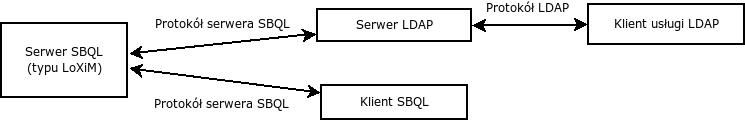
\includegraphics[scale=0.5]{img/ServerSBQLjakoBackendLDAP.jpg}
		\caption{Schemat serwera SBQL jako zaplecza us�ugi LDAP}
	\end{figure}  
	
W schemacie tym mamy zwyk�� baz� danych realizuj�c� dost�p poprzez j�zyk SBQL
oraz serwer LDAP wykorzystuj�cy t� baz� danych jako narz�dzie do przechowywania
i wyszukiwania informacji. Do serwera us�ugi LDAP jest zapewniony dost�p za
pomoc� protoko�u LDAP. Inne systemy chc�ce analizowa� dane przy pomocy SBQL'a
powinny dostawa� si� bezpo�rednio do bazy danych SBQL. 

Jest to najbardziej naturalne rozwi�zanie od strony implementacyjnej i
architektonicznej. Istniej� w nim dwa prawie niezale�ne komponenty skupione na
�wiadczeniu konkretnych us�ug. 

Zastosowanie tego modelu rodzi nast�puj�ce spostrze�enia:
\begin{itemize}
  \item Nie istnieje �adna zale�no�� pomi�dzy protoko�em dost�pu do bazy danych
  SBQL, a protoko�em LDAP. 
  \item Przechowywanie danych poprzez serwery us�ug katalogowych w
  semistrukturalnych, obiektowych bazach danych wydaje si� by� o wiele lepszym
  rozwi�zaniem ni� wykorzystywanie do tego celu relacyjnych baz danych (np.
  oprogramowanie OpenLDAP przechowuje dane w bazie Berkeley DB). Mo�na si�
  spodziewa�, �e z czasem powstan� narz�dzie zorganizowane w ten spos�b.
  \item Opracowanie jednego standardu przechowywania danych us�ug katalogowych
  w bazach typu \loxim{} --- zanim powstan� r�ne realizacje us�ug opartych na tym modelu --- 
  umo�liwi �atwiejsz� wymian� konkretnej implementacji us�ugi LDAP lub budowania
  wielu program�w korzystaj�cych z drzewa typu LDAP poprzez j�zyk SBQL. Dlatego
  w rozdziale ,,Symulowanie modelu danych protoko�u LDAP za pomoc� modelu
  danych SBQL'' (rozdzia� \ref{SymulowanieLDAPbySBQL}) spr�bujemy
  przeanalizowa� dost�pne mo�liwo�ci w tej kwestii.
  \item Istnieje ryzyko, �e modyfikacje danych przeprowadzane za pomoc� j�zyka
  SBQL b�d� narusza�y warunki stawiane strukturze danych serwera SBQL
  symuluj�cej katalog SBQL. Dlatego wskazane jest by taki schemat danych by�
  kontrolowalny pod wzgl�dem sp�jno�ci za pomoc� mechanizm�w serwera SBQL. 
\end{itemize}


\subsubsection{Serwer LDAP �wiadcz�cy dost�p za pomoc� j�zyka SBQL}
	\begin{figure}[hbt]
		\centering
		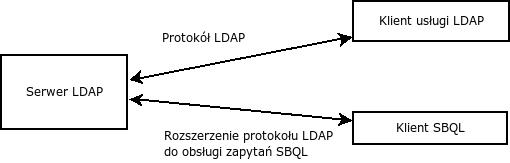
\includegraphics[scale=0.5]{img/ServerLDAPzDostepemSBQL.jpg}
		\caption{Schemat serwera LDAP z dost�pem przez SBQL}
	\end{figure}

Alternatywnym scenariuszem jest sytuacja, w kt�rej obecne rozwi�zania LDAP
zacz�yby by� rozszerzane do obs�ugi j�zyka typu SBQL. Wtedy naturalnym
rozwi�zaniem jest wprowadzenie do protoko�u LDAP rozszerzenia (nowych typ�w
pakiet�w), kt�re umo�liwi� zadawanie zapyta� w j�zyku SBQL, zamiast
implementowania na serwerze LDAP zupe�nie innego protoko�u. 

W realizacji tego rozwi�zania b�dzie potrzebny standard m�wi�cy 
jakiej strukturze danych serwera SBQL odpowiada dany katalog LDAP, a wi�c
opisuj�cy w jaki spos�b wykonywa� zapytania SBQL. Problem ten zosta� 
rozwini�ty w rozdziale \ref{SymulowanieLDAPbySBQL} ,,Symulowanie modelu danych
protoko�u LDAP za pomoc� modelu danych SBQL''. 

Drugim brakuj�cym elementem jest specyfikacja rozszerzenia protoko�u LDAP,
umo�liwiaj�ca w tym protokole wykonywanie zapyta� SBQL. Problemem tym zajmujemy
si� w rozdziale \ref{RozszerzenieLDAP}. 

\subsubsection{Serwer SBQL �wiadcz�cy dost�p do danych za pomoc� protoko�u LDAP}
\begin{figure}[hbt]
	\centering
	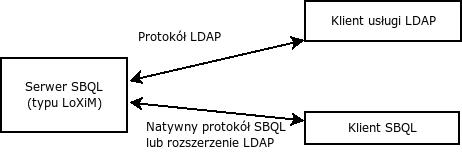
\includegraphics[scale=0.5]{img/ServerSBQLzDostepemLDAP.jpg}
	\caption{Schemat serwera SBQL �wiadcz�cego dost�p do danych za pomoc�
	protoko�u LDAP}
\end{figure}  

W tym modelu rozpatrujemy serwer SBQL, kt�ry nie tylko obs�uguje dost�p za
pomoc� j�zyka SBQL, ale tak�e udost�pnia zasoby za pomoc� mechanizm�w protoko�u
LDAP. Gdyby mo�liwe by�o sensowne wykonywanie wyszukiwa� LDAP oraz polece�
modyfikuj�cych dane protoko�u LDAP na ka�dym modelu danych serwera SBQL (modelu
$AS_0$ lub wy�szego) to realizacja tego modelu mia�a by sens. Umo�liwi�aby ona
wykorzystanie ju� istniej�cych rozwi�za� integruj�cych si� z us�ugami
katalogowymi i operowanie bezpo�rednio na bazie typu \loxim.

Kwestiami wykonywania operacji protoko�u LDAP na og�lnym modelu danych
serwera SBQL ($AS_0$) zajmiemy si� szczeg�owo w rozdziale \ref{OperacjeLDAPw$AS_0$}.

By nie mno�y� byt�w w tym rozwi�zaniu mia�oby sens zastosowanie
jednego protoko�u dost�pu --- kt�rym by�by protok� LDAP wraz z pewnymi
rozszerzeniami umo�liwiaj�cymi wykorzystywanie j�zyka SBQL do przeprowadzania
zapyta�. S� to te same rozszerzenia, kt�re dotycz� ,,Serwera LDAP �wiadcz�cego
dost�p za pomoc� j�zyka SBQL'' i kt�re szczeg�owo omawiamy w rozdziale
\ref{RozszerzenieLDAP}. 
		
\section{Analiza}

\subsection{Por�wnanie modeli danych}

\subsubsection{SBQL}

Rozwa�my najbardziej og�lny model danych dla j�zyka
SBQL --- ($AS_0$ Store Model). W modelu tym obiekty s� 
tr�jkami \triple{identyfikator}{nazwa}{warto��}, w kt�rych wyr�niamy
w trzy przypadki:
\begin{description}
	\item[Obiekty atomowe (proste)] --- (ang. atomic objects)
	\triple{identyfikator}{nazwa}{warto�� prosta}
	\item[Obiekty wska�nikowe] --- (ang. pointer objects)
	\triple{identyfikator}{nazwa}{identyfikator docelowy}
	\item[Obiekty z�o�one] --- (ang. complex objects)
	\triple{identyfikator}{nazwa}{kolekcja obiekt�w}
	Gdzie kolekcja obiekt�w mo�e by� zbiorem (ang. set) b�d�
	sekwencj� (ang. sequence) element�w (w modelu $AS_{0_{seq}}$)
\end{description} 

Model ten narzuca dodatkowo pewne wymagania dotycz�ce ``zgodno�ci'' danych:
\begin{itemize}
	\item Unikatowo�� identyfikator�w obiektu. W ca�ym systemie nie istniej� 
	dwa elementy o takim samym identyfikatorze (pierwszym elemencie tr�jki)
	\item Je�eli obiekt jest typu wska�nikowego, to obiekt na kt�ry wskazuje musi
	istnie�
\end{itemize} 

Dodatkowo obowi�zuje za�o�enie ca�kowicie ukrytego identyfikatora (Total
internal object identification) w ,,Principles of query programming languages'' \cite{SBQL},
kt�re oznacza, �e u�ytkownik (aplikacja kliencka) nie mo�e pozna� identyfikatora
obiektu z kt�rym pracuje. Zatem w tym modelu danych nie istnieje �aden
zewn�trzny identyfikator (adres), kt�ry by potrafi� unikatowo zidentyfikowa�
konkretny obiekt w ca�ej bazie danych implementuj�cej ten model.  

\subsubsection{Model danych LDAP}
	Dane s� reprezentowane w postaci hierarchii obiekt�w (wpis�w) (ang. entries).
	Szczytowe (ang. top) obiekty takiego drzewa nazywane s� korzeniami (ang.
	roots/base/suffixs). Ka�dy obiekt ma maksymalnie jednego ojca i mo�e mie� dowoln� liczb�
	dzieci oraz zbi�r atrybut�w. 
	
	Ka�dy atrybut ma nazw� i mo�e mie�  jedn� lub
	wiele warto�ci. Warto�ci w obr�bie pojedynczego atrybutu nie mog� by� to�same
	 (definicja to�samo�ci zale�y od atrybutu (matching rule). Kolejno�� warto�ci w
	 obr�bie atrybutu o wielu warto�ciach nie ma znaczenia. 
	 Mo�na my�le� o atrybucie z wieloma warto�ciami jak o wielu atrybutach z tak� 
	sam� nazw� i r�nymi warto�ciami. 
	
	Dla r�nych atrybut�w mo�e by� w r�nych spos�b zdefiniowana identyczno��
	(matching rule). W szczeg�lno�ci specyfikacja, czy por�wnanie jest zale�ne
	od wielko�ci znak�w (case sensitive/insensitive) jest najcz�ciej u�ywan�
	w�asno�ci� atrybutu. 
	
	Obiekty od danego korzenia buduj� drzewo DIT (Directory Information Tree). W
	obr�bie drzewa ka�dy obiekt mo�na zaadresowa� za pomoc� DN (Distinguish
	Name). DN buduje si� jako ci�g obiekt�w par: (atrybut=warto��), specyfikuj�cych 
	pe�n� �cie�k� od obiektu do korzenia.
	
	Np. cn=Piotr Tabor,ou=MIMUW,o=UW,city=Warszawa,country=Polska.
	
	Protok� LDAP przewiduje istnienie alias�w, kt�re polegaj� na tym, �e 
	element mo�e pokazywa� na Distinguish Name innego elementu. Z punktu widzenia
	przeszukiwania (o ile flaga dereferencji alias�w w zapytaniu jest w��czona)
	taki element jest traktowany jakby nale�a� do poddrzewa. Linki te mo�na
	rozumie� jako analogi� do dowi�za� symbolicznych w systemach Uniksowych.
	
	
	\begin{figure}[hbt]
		\centering
		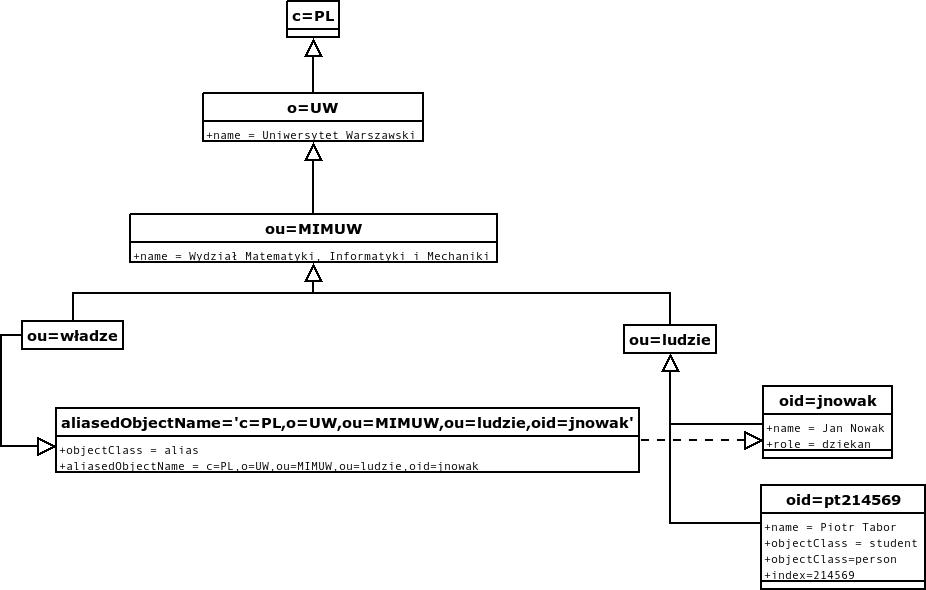
\includegraphics[scale=0.5]{img/ldap_mimuw.jpg}
		\caption{Przek�ad 1 danych w modelu LDAP}
	\end{figure}  

% \subsection{Por�wnanie cech obu modeli}
% 
% \begin{tabular*}{17cm}{|l|l|l|}
% 	\hline
% 	\bf{Cecha} & \bf{LDAP} & bf{$AS_0$ (SBQL)} \\
% 	\hline
% 	
% 	Jednostki danych & Atrybuty, dzieci &  Uto�samione zosta�y atrybuty i
% 	podobiekty (dzieci)\\
% 	
% 	Identyfikacja	 & 
% 	
% 	Aliasy 			 &	
% \end{tabular*} 

	
\subsection{Symulowanie modelu danych protoko�u LDAP za pomoc� modelu
danych SBQL}
\label{SymulowanieLDAPbySBQL}
\subsubsection{Podej�cie 1}

Na podstawie danych w modelu LDAP mo�na zbudowa� ich instancj� w modelu $AS_0$
w nast�puj�cy rekurencyjny spos�b (za��my, �e mamy zbudowa� struktur� dla
poddrzewa zaczynaj�cego si� w danym wpisie E):

Tworzymy obiekt okalaj�cy o id ($i_1$), zawieraj�ce nast�puj�cy wi�zania
 (bindings):
 	\begin{description}
 		\item[entry] --- obiekt (wpis) w�a�ciwy.
 			\begin{itemize}
 				\item Dla ka�dego atrybutu nale��cego do wpisu E tworzymy wi�zanie o nazwie
 				atrybutu prowadz�ce do warto�ci tego atrybutu.
 			
 				\item  Dla atrybutu kluczowego (buduj�cego 	,,distinguish name'') tworzymy
 				wi�zanie o nazwie atrybutu poprzedzonej '\#' prowadz�ce do warto�ci
 				atrybutu kluczowego.
 				
 				\item Dla ka�dego wpisu bezpo�rednio podleg�ego tworzymy binding o nazwie
 				'\#child\#' prowadz�cy do rekurencyjnie wygenerowanego dla
 				tego wpisu obiektu okalaj�cego. 
			\end{itemize}
 		\item[deref] -
 			Je�eli bie��cy wpis jest aliasem to ,,deref'' wskazuje na cel aliasu
 			(bezpo�rednio, a nie na obiekt okalaj�cy). W przeciwnym przypadku wi��e do
 			tego samego obiektu co ,,entry''.
	\end{description}


Przyk�ad z rysunku przedstawionym w ``Modelu danych LDAP'', zapisany w $AS_0$ z
wykorzystaniem tego podej�cia (po dodaniu nadrz�dnych obiekt�w root i
\#child\#): \begin{verbatimtab}[3] 1 root:
	2 #child#:
		3 deref: ->5
		5 entry:
			6 c=PL
			7 #c -> 6
			8 #child#:
				9 deref: ->10
				10 entry:
					11 ou=UW
					12 #ou -> 11
					13 name=Uniwersystet Warszawski
					14 #child#:
						15 deref: ->16
						16 entry: 
							17 ou=MIMUW
							18 #ou=MIMUW
							19 name=Wydzia� Matematyki, Informatyki i Mechaniki
							20 #child#
								21 defer: ->22
								22 entry: 
									23 ou=ludzie
									24 #ou ->23
									25 #child#
										26 deref ->27
										27 entry:
											28: oid=jnowak
											29: #oid ->28
											30: name=Jan Nowak
											31: objectClass: person
											50: role: dziekan
									32 #child#
										33 deref ->34
										34 entry:
											35: oid=pt214569
											36: #oid ->35
											37: name=Piotr Tabor
											38: index=214569
											39: objectClass: person
											40: objectClass: student
							41 #child#
								42 deref: ->43
								43 entry: 
									44 ou=W�adze
									45 #ou ->44 
									46 #child#:
										47 deref ->27
										48 entry:
											49 aliasedObjectName='c=PL,o=UW,ou=MIMUW,ou=ludzie,oid=jnowak'	
											51 #aliasedObjectName ->49
											52 objectClass: alias										
\end{verbatimtab}

W tym modelu mo�emy stosunkowo �atwo przet�umaczy� ,,distinguish name'' na
zapytanie odnajduj�ce wskazany adres.
Nast�puj�cy adres: c=PL,o=UW,ou=MIMUW,ou=ludzie,oid=jnowak zostanie
przet�umaczony na:
\begin{description}
	\item[W przypadku nie rozwijania alias�w]:\\
	(root).(entry where \#c=PL).\#child\#.(entry where \#ou=UW).\#child\#\\
	.(entry	where \#ou=MIMUW).\#child\#.(entry where \#ou=ludzie).\#child\#\\
	.(entry where \#oid=pt214569).\#child\#
	\item[W przypadku rozwijania alias�w]:\\
	(root).(deref where \#c=PL).\#child\#.(deref where \#ou=UW) .\#child\#\\
	.(deref	where \#ou=MIMUW).\#child\#.(deref where \#ou=ludzie).\#child\#\\
	.(deref where \#oid=pt214569).\#child\# 
\end{description}

% \subsubsection{Podej�cie 2}
% 
% Wydaje si� istotnym post�pem, gdyby uda�o si� z podej�cia pierwszego usun��
% obiekty okalaj�ce. Tak naprawd� jedynym powodem, dla kt�rego je wprowadzili�my
% by�a konieczno�� rozr�niania przej�cia po wi�zaniu zwyk�ym
% (typu \triple{$i_1$}{name}{[zbi�r obiekt�w]}), a wi�zaniu typu wska�nik/link 
% (typu \triple{$i_1$}{name}{$i_2$}). Gdyby j�zyk SBQL wprowadzi� operator
% algebraiczny $is_pointer(i)$


\subsection{Operacje protoko�u LDAP} \label{OperacjeLDAPw$AS_0$}
	\subsubsection{Operacje protoko�u StartTLS}

		Wys�anie paczki StartTLS przez klienta protoko�u LDAP powoduje rozpocz�cie negocjacji TLS (Transport Layer Security), czyli
		bezpiecznego --- szyfrowanego --- po��czenia. Operacja ta jest istotna i w oczywisty spos�b �atwa do zaimplementowania
		w przypadku wykorzystania protoko�u do komunikacji z innym rodzajem bazy danych. 
	
	\subsubsection{Bind --- autoryzacja}

W protokole LDAP klient przeprowadzaj�c autoryzacj� przekazuje nast�puj�ce parametry serwerowi:
\begin{description}
	\item[wersje protoko�u] --- po kt�rej chce si� komunikowa� (obecnie dozwolona tylko wersja 3)
	\item[nazwa (DN) loguj�cego si�] --- adres (DN) wpisu identyfikuj�cego obiekt autoryzuj�cy si� (przewa�nie u�ytkownika)
	\item[dane autentykuj�ce] --- paczka danych opisuj�cych wybran� metod� autentykacji oraz zestaw danych potrzebnych do jej przeprowadzenia.
	Specyfikacja podstawowych metod znajduje si� w dokumencie \cite{RFC4520} i przewiduje: logowanie anonimowe, logowanie z podaniem loginu i has�a
	(czystego b�d� zaszyfrowanego) oraz us�ugi SASL (Simple Authentication and Security Layer). 
\end{description}   

Wykorzystanie tej metody w modelu bazy semistrukturalnej niesie ze sob� nast�puj�ce trudno�ci:
\begin{itemize}
  \item Zak�ada, �e u�ytkownicy bazy danych s� dost�pni jako element struktury danych. To za�o�enie wydaje
  si� sensowne. W najgorszym przypadku u�ytkownicy mog� by� udost�pniani jako fragment wirtualnego modelu danych (analogia do
  katalogu /proc w UNIX'ach).
  \item Zak�ada, �e dysponujemy mechanizmem t�umaczenia adres�w DN na konkretne obiekty modelu $AS_0$ (\patrz{SymulowanieLDAPbySBQL}) (w og�lnym przypadku danych -
  niemo�liwe lub bardzo si�owe)
\end{itemize}

Drugie z wymieniony za�o�e� jest problemem trudnym, ale przyjmuj�c nawet, �e jest nierozwi�zywalny z niewielk� strat� 
mo�emy przyj��, �e operacja BIND z atrybutem name=``o=loxim,cn=kowalski'' odpowiada pr�bie autentykacji u�ytkownika Kowalski do bazy danych. 

Reasumuj�c --- pakiet ten jest istotny i mo�liwe jest jego wykorzystanie przy dost�pie do bazy danych typu \loxim.  

\subsubsection{Unbind --- zako�czenie po��czenia}
Nazwa tego polecenia jest myl�ca, gdy� w protokole LDAP oznacza ona operacje zamkni�cia po��czenia 
(a nie --- jak mog�a by sugerowa� --- wylogowania u�ytkownika). 

Operacja nie niesie ze sob� �adnych trudno�ci w dost�pie do danych o semistrukturalnym modelu. 

\subsubsection{Search --- wyszukiwanie}
Operacja ,,search'' jest najwa�niejsz� operacj� w us�ugach katalogowych. Przyjmuje nast�puj�ce parametry: 
\begin{description}
	\item[baseObject] --- adres (DN) miejsca w drzewie od kt�rego (w g��b) rozpoczynamy przeszukiwanie
	\item[scope]      --- zakres drzewa, kt�ry chcemy przeszuka�:
		\begin{description}
			\item[baseObject] --- przeszukany zostaje tylko wskazany obiekt (w praktyce oznacza to sprawdzenie, czy wskazany obiekt spe�nia zadane warunki lub pobranie
			wybranych atrybut�w z obiektu)
			\item[singleLevel] --- przeszukane zostaj� (bezpo�rednie) dzieci danego obiektu
			\item[wholeSubtree] --- przeszukane zostaje ca�e poddrzewo wyznaczone przez ,,baseObject'', czyli wszyscy potomkowie tego obiektu z nim w��cznie  
		\end{description}
	\item[derefAliases] --- jak aliasy (odpowiednik obiekt�w pointerowych) maj� by� traktowane:
		\begin{description}
			\item[neverDerefAliases]   --- nigdy nie interpretuj alias�w 
			\item[derefInSearching]    --- interpretuj aliasy tylko w trakcie przeszukiwania (ale nie w trakcie znajdowania ,,korzenia przeszukiwania'' (baseObject))
			\item[derefFindingBaseObj] --- interpretuj aliasy w trakcie znajdowania ,,korzenia przeszukiwania'' (baseObject)
			\item[derefAlways]         --- zawsze interpretuj aliasy
		\end{description}
	\item[sizeLimit] --- maksymalna liczba zwr�conych wpis�w
	\item[timeLimit] --- maksymalny czas przeszukiwania (w sekundach). W przypadku przekroczenia --- zwr�cone zostan� wpisy znalezione do czasu jego up�yni�cia. 
	\item[typesOnly] --- true lub false --- decyduje, czy zapytanie zwraca pary: opis atrybutu i jego warto��, czy tylko opisy atrybut�w 
	\item[filters] --- z�o�ony obiekt reprezentuj�cy warunki jakie musz� spe�nia� zwr�cone wpisy (obejmuje: por�wnania atrybut�w ze sta�ymi (tak�e przybli�one),
	operacje logiczne, sprawdzanie istnienia atrybutu). 
	\item[attributes] --- lista atrybut�w, kt�re maj� zosta� zwr�cone dla ka�dego znalezionego wpisu. Mo�na te� przekaza� warto�� ��daj�c� wszystkich atrybut�w
	zawartych w danym wpisie (bez ukrytych). 
\end{description} 

W odpowiedzi na t� operacj� b�d� przychodzi� (asynchronicznie): lista znalezionych obiekt�w z warto�ciami wskazanych atrybut�w --- a tak�e 
lista serwer�w, kt�re mog� zna� wi�cej odpowiedzi na to zapytanie (mo�e by� warto przeprowadzi� to samo przeszukiwanie
na nich, ale to decyzja klienta). 

Wykorzystanie tego mechanizmu do przeszukiwania bazy danych opartej na j�zyku SBQL wymaga:
\begin{itemize}
  \item przet�umaczenia adresu ,,baseObject'' na konkretny obiekt modelu $AS_0$ (czyli na zapytanie SBQL znajduj�ce ten obiekt) (\patrz{SymulowanieLDAPbySBQL}) z
  interpretacj� (lub nie) alias�w --- w zale�no�ci od warto�ci parametru ,,derefAliases'' (w og�lnym przypadku danych --- niemo�liwe lub bardzo si�owe) 
  \item  Przet�umaczenie warunk�w wyszukiwania zadanych parametrem ,,filter'' na SBQL'a --- uwzgl�dniaj�cego wybrany ,,scope'', a tak�e rozwijanie alias�w
  (,,deref aliases''). Zak�adaj�c, �e mo�emy sk�adnie SBQL'a rozszerzy� o funkcje dokonuj�ce bardziej z�o�onych por�wna� (np. z uwzgl�dnieniem skr�t�w MD5 lub
  SHA1) co wydaje si� w pe�ni realizowalne --- o ile wiemy jak interpretowa� poj�cie ,,wpis'' i ,,atrybut'' w kontek�cie przetwarzanych danych ($AS_0$). 
\end{itemize}

Problemy te --- je�li zak�adamy, �e baza danych zawiera dane w og�lnym modelu $AS_0$ wydaj� si� uniemo�liwia� przeprowadzenie tej operacji. Jednak na danych, kt�re
potrafimy zinterpretowa� jako ,,wpisy'' i ,,atrybuty'' mo�emy z powodzeniem i wydajnie zaimplementowa� t� operacj�. 

Operacja ta nie nadaje si� do zadawania zapyta� w j�zyku SBQL w szczeg�lno�ci ze wzgl�du na stosunkowo ,,p�aski'' format odpowiedzi, a tak�e  braku 
parametru umo�liwiaj�cego wygodne przekazanie zapytania SBQL wraz z warto�ciami jego parametr�w. Z tego wzgl�du --- je�li chcemy zapewni� mo�liwo�� zadawania
zapyta� SBQL bazie danych --- musimy zaimplementowa� now� operacj� do tego przeznaczon� (rozszerzenie protoko�u LDAP).  

\subsubsection{Modify --- zmiana wpisu}
Operacja ,,modify'' umo�liwia klientowi dodanie lub usuni�cie atrybut�w z wpisu, a tak�e zamian� warto�ci wskazanych atrybut�w. 
Zawiera dwa parametry:
\begin{description}
	\item[object] --- adres (DN) wpisu, kt�ry chcemy zmodyfikowa�. 
	\item[changes] --- list� operacji modyfikacji.
	Operacjami modyfikacji mo�e by�:
		\begin{description}
			\item[add]  --- dodanie atrybutu (lub warto�ci do atrybutu --- je�li ten ju� istnieje)
			\item[delete] --- usuni�cie ca�ego atrybutu (lub pojedynczej warto�ci --- je�li zosta�a ona wskazana) 
			\item[replace] --- zamienienie wszystkich warto�ci wskazanego atrybuty na za��czone do tej operacji. 
		\end{description}
\end{description} 

Przeprowadzenie tej operacji w bazie typu SBQL jest mo�liwe w sytuacji kiedy umiemy mapowa� poj�cia ,,wpis'' i ,,atrybut'' na model danych.
W og�lnym przypadku musimy odnale�� ,,object'' (czyli przet�umaczy� DN na zapytanie SBQL), a nast�pnie w zale�no�ci od wybranej operacji 
musieliby�my usun��, zmodyfikowa� lub doda� nowe dziecko typu ,,binder'' do wskazanego obiektu. Tworzony binder b�dzie zwi�zany z warto�ci� typu
prostego. 

\subsubsection{Add --- dodanie wpisu}

Operacja przyjmuje dwa parametry: adres (DN) wpisu, kt�ry chcemy utworzy� oraz list� atrybut�w wraz z warto�ciami dla tego obiektu.

Przy za�o�eniu, �e umiemy przet�umaczy� DN na obiekt modelu $AS_0$, kt�ry chcemy utworzy� --- operacj� t� 
mo�emy wykona� przez utworzenie prostego obiektu typu ,,binder'' dla ka�dego atrybutu we wskazanym obiekcie.  

\subsubsection{Delete --- usuni�cie wpisu}

Operacja usuwa wskazany wpis. Jej jedynym parametrem jest DN wpisu, kt�ry chcemy usun��. 

Przy za�o�eniu, �e umiemy przet�umaczy� DN na obiekt modelu $AS_0$, kt�ry chcemy usun�� --- ta operacja jest wykonywalna i istotna.  


\subsubsection{Abandon --- przerwanie przetwarzanej w�a�nie operacji}

Operacja ta przyjmuje parametr b�d�cy id wykonywanej aktualnie operacji (przewa�nie polecenia SEARCH) i wymusza jej zako�czenie. 

Operacja istotna i mo�liwa do implementacji w bazie danych opartej na SBQL.  

%\subsubsection{Symulowanie operacji protoko�u LDAP na bazie danych w modelu $AS_0$}
%\label{OperacjeLDAPw$AS_0$}

% \subsection{Zgodno��}
% 	Mo�liwe jest, by system \loxim{} realizowa� wszystkie powy�sze operacje, a tym
% 	samym by� ``pe�nym'' serwerem us�ugi katalogowej w rozumieniu protoko�u LDAP.
% 	
% 	Operacj� search, modify, delete i add bez wi�kszych problem�w mo�na
% 	przet�umaczy� na j�zyk SBQL. Jedynym wymaganiem jest, by SBQL
% 	implementowa� nast�puj�ce funkcje:
% 	\begin{description}
% 		\item[approxMatch] (RFC4511 (4.5.1.7.5)) --- zwracaj�c�,  czy dwa dane elementy
% 			,,prawie'' (np. fonetycznie, leksykalnie) do siebie pasuj�. Mo�na te� u�y�
% 			operacji ,,r�wna si�'' do najprostszej implementacji tej funkcji (t�umacz
% 			LDAP $\to$ SBQL przet�umaczy j� jako ,,r�wna si�``)
%     \end{description}
% 	
% 	Szczeg�lnie interesuj�ce wydaje si� po��czenie mo�liwo�ci relacyjnych baz
% 	danych (transakcje, skomplikowane regu�y wyszukiwania i aktualizacji danych) i
% 	us�ug katalogowych w jednym narz�dziu.
	

\subsection{Podsumowanie}

Pomimo wielu cech wsp�lnych obu narz�dzi \patrz{wspolne} wykorzystanie
czystego protoko�u LDAP jako jedynego interfejsu komunikacyjnego jest problematyczne.

Wykazali�my, �e operacje ,,bind'', ,,unbind'', ,,startTLS'', ,,abandon'' mo�na stosunkowo 
�atwo wykorzysta� w bazie danych typu SBQL (mo�na je wykorzysta� w ka�dym protokole, kt�ry
przeprowadza autentykacje). Stanowi� one ,,standardowy'' szkielet, na kt�rym mo�na budowa� 
protok� w�a�ciwy. 

Operacje ,,add'', ,delete'' i ,,modify'' jeste�my w stanie przeprowadzi� w bazie danych typu \loxim{} o ile 
potrafimy zinterpretowa� DN jako adres konkretnego obiektu w tej bazie. W praktyce jest to tylko mo�liwe je�li
baza u�ywa schematu, kt�ry jeste�my wstanie zinterpretowa� jako zgodny z us�ug� LDAP \patrz{SymulowanieLDAPbySBQL}.

Operacja ,,search'' jest tak�e tylko mo�liwa, gdy dane bazy danych potrafimy zobrazowa� jako zgodne z us�ug� LDAP.

Do przeprowadzania zapyta� i modyfikacji przy pomocy j�zyka SBQL b�dziemy potrzebowali wprowadzi� rozszerzenie protoko�u LDAP 
(wprowadzanie rozszerze� jest przewidziane przez ten standard).

\subsubsection{Wizja realizacji}
	W tym podpunkcie przedstawi� pomys� na maksymaln� integracj� bazy danych SBQL i protoko�u LDAP, kt�ra ma sens: 
	
	\begin{enumerate}
		\item Dost�p do takiej bazy danych by�by realizowany przez protok� LDAP z dodatkowymi pakietami umo�liwiaj�cymi
		wykonywanie parametryzowanych zapyta� SBQL.
		\item W schemacie bazy danych powinny istnie� wyr�nione poddrzewa, kt�ry maj� okre�lon� struktur� --- zgodn� ze schematem us�ugi LDAP (najlepiej kontrolowan�
		poprzez model np. $AS_1$ lub wy�sze). Dost�p do tych danych (i tylko nich) powinien by� zapewniony poprzez operacje ,,Search'', ,,Add'' , ,,Delete'' i
		,,Modify''.
		\item Do ca�ego schematu bazy danych powinien istnie� dost�p za pomoc� j�zyka SBQL przy pomocy rozszerzenia protoko�u om�wionego w punkcie 1.  	
	\end{enumerate}    

	Takie rozwi�zanie ma nast�puj�ce zalety:
	\begin{itemize}
      \item U�atwiamy �ycie programistom narz�dzi klienckich --- kt�rzy mog� wykorzysta� ju� istniej�cy (dla protoko�u LDAP) kod do autentykacji.
      \item Korzystamy z bogactwa metod autentykacji przygotowanych ju� dla protoko�u LDAP.
      \item U�atwiamy integracj� wszystkich danych w pojedynczym narz�dziu ze sp�jnym interfejsem.   
      \item U�atwiamy migracj� ze standardowego modelu ,,LDAP + baza danych''  do modelu ,,SBQL z interfejsem LDAP''.
      \item Nie tworzymy ,,nowych (wcale nie lepszych) standard�w'' w informatyce.
      \item Umo�liwiamy wsp�prac� bazy typu \loxim{} z wieloma ju� istniej�cymi aplikacjami i bibliotekami. 
    \end{itemize}

% 
% Wady protoko�u LDAP przy omawianym zastosowaniu:
% \begin{itemize}
%   \item --- Brak natywnej mo�liwo�ci zadawania zapyta� w j�zyku SBQL 
% \end{itemize}
% 
% Protok� LDAP przewiduje mo�liwo�� wprowadzania rozszerze�.

%\section{Proponowane rozszerzenia protoko�u LDAP}
\label{RozszerzenieLDAP}


	
\chapter{\dokprotogen}\label{dokprotogen}
	\section{Wprowadzenie}

\subsection{Wst�p}

Generator protoko��w jest narz�dziem s�u��cym do generowania implementacji
protoko�u sieciowego w r�nych j�zykach programowania w oparciu o zadany opis. 
Danymi wej�ciowymi generatora jest specyfikacja protoko�u zapisana w pliku XML
(patrz: \ref{xml}) oraz wybrany j�zyk programowania. Danymi wyj�ciowymi jest 
kod �r�d�owy w wybranym j�zyku programowania umo�liwiaj�cy wygodne pos�ugiwanie
si� tym protoko�em.

\subsection{Licencjonowanie}

Projekt ,,ProtoGen 1.0'' jak i wygenerowany przez niego kod jest licencjonowany
na zasadach licencji ,,Apache Software License 2.0''
(http://www.apache.org/licenses/LICENSE-2.0).

\subsection{Korzy�ci p�yn�ce ze stosowania tego rozwi�zania}

Zastosowanie tego narz�dzia daje nast�puj�ce korzy�ci:
\begin{itemize}
  \item Gwarantuje zgodno�� na poziomie danych przysy�anych sieci� dla
  implementacji w r�nych j�zykach programowania
  \item Pozwala unikn�� programi�cie ,,mechanicznego'' tworzenia du�ych ilo�ci
  kodu a zaraz b��d�w z tym zwi�zanych
  \item Gwarantuje, �e ca�y kod protoko�u jest napisany w spos�b sp�jny
  \item Gwarantuje, �e wygenerowany kod jest odporny na podstawowe zagro�enia w
  komunikacji pomi�dzy r�nymi architekturami: problem kolejno�ci bajt�w w
  s�owie (big-endian/little-endian) oraz problem rozmiaru podstawowych typ�w
  danych (architektury od 8 do 64 bit�w).
  \item Tworzy zestawy test�w, kt�re
  umo�liwiaj� sprawdzanie komunikacji tak�e pomi�dzy kodem wygenerowanym dla
  r�nych j�zyk�w programowania. 
  \item Umo�liwia aktualizacj� ca�ego modu�u poprzez aktualizacj� generatora i
  ponowne wygenerowanie kodu. 
\end{itemize}

\subsection{Ograniczenia rozwi�zania}

ProtoGen nie jest narz�dziem, kt�re umo�liwia wygenerowanie modu�u
obs�uguj�cego ka�dy protok�. W obecnej wersji zosta�y przyj�te poni�sze
ograniczenia.

\subsubsection{Budowa paczki}

		Ka�da paczka ma nast�puj�cy schemat budowy:
		\begin{bajty}
                	\bp{0}{$a$}{'zale�y od konfiguracji'}{Sta�a m�wi�ca o typie
                	paczki, a tym samym okre�laj�ca format zawartych w nich danych}
                	\bp{$a+1$}{$a+4$}{uint32}{n- Sta�a okre�laj�ca
                	ilo��
                	danych w�a�ciwych zawartych w paczce - wyra�ona w bajtach}
                	\bp{$a+5$}{$a+5+n$}{patrz opis zale�ny od typu paczki}{Dane
                	w�a�ciwe paczki zgodne z formatem okre�lonym poprzez typ paczki}
 		    \end{bajty}	
		Formalnie b�dziemy m�wili, �e paczka si� sk�ada z dwu-polowego nag��wka oraz
		cia�a. Nag��wek wyznacza typ paczki i rozmiar danych w�a�ciwych w niej
		zawartych, a cia�o - to dane interpretowane zale�nie od typu paczki. 
		
		
\subsubsection{Big/endian - little/endian}
Przyj�to, �e wszystkie dane s� przesy�ane przez sie� w formacie big-endian.

\subsubsection{Format napis�w}
Przyj�to, �e wszystkie napisy s� przesy�ane przez sie� w formacie UTF-8. 

\subsection{Z�o�ona logika}
	
	Obecnie ProtoGen nie wspiera z�o�onej logiki w konstrukcji pakiet�w. Niemo�liwe jest warunkowanie istnienia pola w zale�no�ci od warto�ci innego pola,
	a tak�e tworzenia tablicy p�l. Obecnie ProtoGen przewiduje mo�liwo��
	nadpisania wygenerowanego kodu. W ten spos�b - nadpisuj�c kod obs�ugi
	odpowiedniej paczki - mo�na uzyska� obs�ug� dowolnie z�o�onej logiki.

	O planowanym rozwi�zaniu tego problemu w przysz�ych wersjach mo�esz przeczyta�
	w rozdziale ,,Dalszy rozw�j'' (patrz: \ref{roadmap})		 	

\newpage
\section{Dokumentacja u�ytkownika}
	\subsection{Uruchomienie}
	
	ProtoGen uruchamiamy b�d�c w katalogu w kt�rym znajduj� si� jego pliku
	uruchomieniowe. W zale�no�ci od systemu operacyjnego uruchamiamy protoGen.sh
	(UNIXy), b�d� protoGen.bat (MS Windows) podaj�c nast�puj�ce parametry:
	\begin{description}
		\item[�cie�ka do deskryptora] - �cie�ka do deskryptora xml opisuj�cego
		protok� (mo�e by� wzgl�dem bie��cego katalogu). Wskazany plik powinien by� w formacie
		opisanym w rozdziale \ref{xml}. 
		\item[�cie�ka do katalogu docelowego] - �cie�ka do katalogu w kt�rym b�d�
		umieszczane wygenerowane pliki. 
		\item[j�zyk docelowy] - j�zyk do kt�rego generujemy kod. Obecnie obs�ugiwane
		warto�ci tego parametru to: ,,cpp'' dla C++ oraz ,,java''. 
		\item[�cie�ka do katalogu z plikami nadpisuj�cymi] (parametr opcjonalny)  -
		parametr s�u�y do wskazania katalogu w kt�rym powinny si� znajdowa� pliki, kt�rymi
		chcemy nadpisa� dzia�anie generatora protoko�u. Mo�e si� zdarzy� sytuacja w
		kt�rej protoGen generowa�by plik ,,ABC.xxx''. Je�eli we wskazanym katalogu
		b�dzie si� znajdowa� plik ,,ABC.xxx'' to on w�a�nie zostanie u�yty zamiast
		wygenerowanego pliku. Pliki umieszczamy w tym katalogu bezpo�rednio (bez
		podkatalog�w). 
		
		Konieczno�� nadpisania pliku pojawia si� najcz�ciej w sytuacji, gdy mamy
		paczk� zawieraj�c� skomplikowan� logik�. Wtedy piszemy kod obs�ugi takiej
		paczki r�cznie, a nast�pnie zmuszamy protoGen, by go wykorzysta� (umie�ci� w
		kodzie wynikowym).
    \end{description}

	\subsubsection{Przyk�ad}
	
	Polecenie:\\
		
	./protoGen.sh ./conf/loxim.xml ./cpp\_proto cpp ./conf/overwritten/cpp\\
	
	 Spowoduje wygenerowanie kodu w j�zyku C++ w podkatalogu cpp\_proto, w oparciu 
	 o deskryptor ./conf/loxim.xml -  sprawdzaj�c, czy istniej� nadpisuj�ce pliki w
	 katalogu ./conf/overwritten/cpp. 
		
	
	\subsection{Format deskryptora protoko�u} \label{xml}
	
	Poni�ej znajduje si� przyk�adowy deskryptor z opisem
	poszczeg�lnych znacznik�w. 
		
	\subsubsection{Przyk�adowy deskryptor}

\lstset{language=xml,tabsize=2,breaklines=true,showspaces=false,showstringspaces=false,showtabs=false}
\lstinputlisting{src/example.xml}

\subsubsection{\znacznik{protocol}}
	\begin{figure}[hbt]
		\centering
			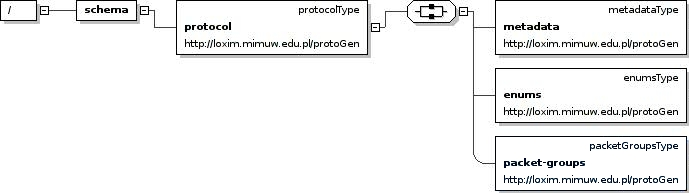
\includegraphics[scale=0.7]{xml/protocol_level.jpg}
		\caption{Konstrukcja znacznika \znacznik{protocol}}
	\end{figure}
	Element \znacznik{protocol} grupuje znaczniki:
	\begin{description}
		\item[\znacznik{metadata}] - opisuj�ce og�lne cechy wygenerowanego protoko�u, a
		tak�e specyficzne cechy zale�ne od docelowego j�zyka programowania.
		\item[\znacznik{enums}] - opisuje typy wyliczeniowe, kt�re mog� zosta� zastosowane
		w protokole. 
		\item[\znacznik{packet-groups}] - opisuje grupy paczek (a zatem te� paczki),
		kt�re, b�d� buduj� protok� bezpo�rednio, b�d� mog� by� elementami sk�adowymi
		paczek. 
    \end{description}

\subsubsection{\znacznik{metadata}}
	\begin{figure}[hbt]
		\centering
			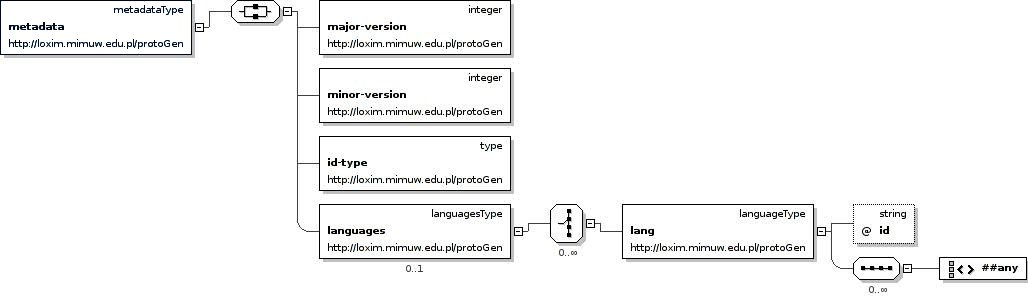
\includegraphics[scale=0.45]{xml/metadata_level.jpg}
		\caption{Konstrukcja znacznika \znacznik{metadata}}
	\end{figure}
	Element \znacznik{metedata} s�u�y opisaniu pewnych og�lnych w�asno�ci protoko�u.
	\begin{description}
		\item[major-version]G��wna wersja protoko�u opisanego w tym deskryptorze.
		Przyjmuje si�, �e protoko�y o tym samym g��wnym numerze wersji s� ze sob�
		kompatybilne (co nie znaczy, �e mo�na za pomoc� nich przekaza� te same
		informacje, ale to �e obie implementacj� b�d� rozmawia�y tak, jakby
		implementowa�y t� sam� - starsz� - wersj� protoko�u). 
		\item[minor-version]Poboczny numer wersji protoko�u.
		\item[languages]Definicja cech protoko�u zale�nych od docelowego j�zyka
		programowania w kt�rym b�dziemy generowali kod. Szczeg�y opisano poni�ej. 
    \end{description}

\subsubsection{\znacznik{lang id="java"}} \label{java-packageName}
	Znacznik ten opisuje dodatkowe atrybuty potrzebne do wygenerowania protoko�u dla j�zyka 
	Java.
		
	\begin{description} 
		\item[packageName]~\\ Nazwa pakietu (jako grupy klas w j�zyku Java)
		zawieraj�cego kod protoko�u. Nale�y oddzieli� wszystkie elementy �cie�ki przy pomocy symbolu '.'. \\
		Wpisana tu nazwa b�dzie tak�e \znacznik{groupId} w utworzonym projekcie Maven2 
		(http://maven.apache.org).
		\item[artifactId]~\\ Nazwa utworzonego modu�u - g��wnie na potrzeby Maven2. 
		\item[version]~\\ Wersja utworzonego modu�u - g��wnie na potrzeby Maven2.  
	\end{description}
	
\subsubsection{\znacznik{lang id="cpp"}}
	J�zyk C++ nie posiada w obecnej wersji ProtoGen dodatkowych atrybut�w. 
	
\subsubsection{\znacznik{enums}} \label{enum}
	\begin{figure}[hbt]
		\centering
			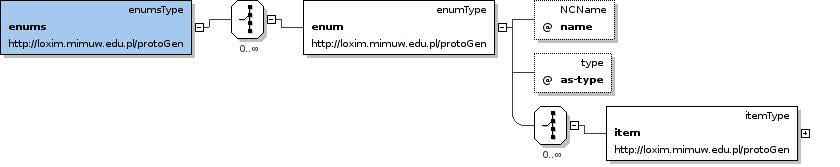
\includegraphics[scale=0.60]{xml/enums.jpg}
		\caption{Konstrukcja znacznika \znacznik{enums}}
	\end{figure}

	Znacznik enums opisuje typy wyliczeniowe, kt�re mog� zosta� wykorzystane w
	protokole. Typy wyliczeniowe mo�na wykorzysta� bezpo�rednio - jako pole 
	zawieraj�ce jedn� warto�� z wielu, a tak�e do stworzenia ,,mapy warto�ci'',
	czyli do przechowania zbioru warto�ci (patrz: \ref{enum-map}). 
	
	\begin{figure}[hbt]
		\centering
			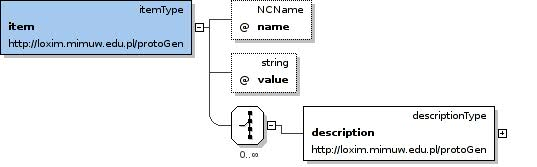
\includegraphics[scale=0.8]{xml/item.jpg}
		\caption{Konstrukcja znacznika \znacznik{item}}
	\end{figure}
	
	Ka�dy element (\znacznik{item}) danego typu wyliczeniowego ma przypisan� warto��
	typu ca�kowitoliczbowego. Je�li chcemy dany typ wyliczeniowy wykorzysta� jako
	,,map�'' to musimy nada� poszczeg�lnym elementom warto�ci o bitach zapalonych
	roz��cznie.
	
	Znacznik \znacznik{enum} opisuje pojedynczy typ wyliczeniowy.
	 
	Jego atrybuty to:
	\begin{description}
		\item[name]    Nazwa typu wyliczeniowego. Przy pomocy tej nazwy b�dzie mo�na
		si� odwo�ywa� do tego typu. Od tej nazwy zale�y te� nazwa wygenerowanej klasy
		przechowuj�cej ten typ. 
		\item[as-type] Nazwa typu numerycznego (patrz: {\ref{typy}}), na kt�ry b�d�
		odwzorcowywane poszczeg�lne enumy. 
    \end{description}

	Ponadto znacznik \znacznik{enum} buduj� elementy \znacznik{item}.  
	
\subsubsection{\znacznik{item}}
	Znacznik item opisuje pojedyncz� warto��, kt�r� mo�e przyj�� typ wyliczeniowy.
	Pojedyncza warto�� posiada nast�puj�ce atrybuty:
	\begin{description}
		\item[name]  Nazwa elementu typu wyliczeniowego.
		\item[value] Warto�� na kt�r� ten element wyliczeniowy b�dzie odwzorowywany.
		Powinna mie�ci� si� w zakresie typu wskazanego w atrybucie ,,as-type'' w znacznika
		\znacznik{enum} definiuj�cym ten typ wyliczeniowy. Warto�� mo�e by� podana
		w systemie dziesi�tnym lub 16-tkowym poprzez poprzedzenie jej symbolami
		,,0x'', np. 0x000f4 - co jest szczeg�lnie przydatne przy konstrukcji typ�w
		u�ywanych do budowania mapy warto�ci (patrz: \ref{enum-map}). 
	\end{description}
	
	Ponadto znacznik \znacznik{item} mo�e posiada� elementy typu \znacznik{description}
	zawieraj�ce dane do budowania dokumentacji (patrz: \ref{description}).

\subsubsection{\znacznik{packet-groups}}
	\begin{figure}[hbt]
		\centering
			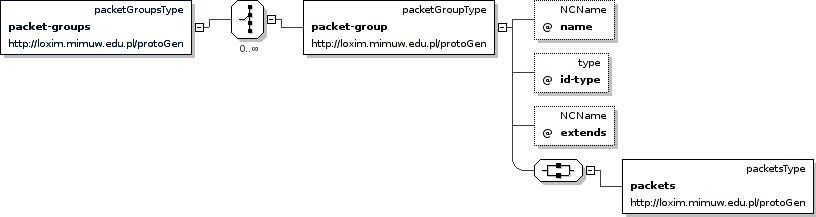
\includegraphics[scale=0.6]{xml/packets_groups_level.jpg}
		\caption{Konstrukcja znacznika \znacznik{packet-groups}}
	\end{figure}

	Znacznik \znacznik{packet-groups} grupuje znaczniki \znacznik{packet-group}, kt�re stanowi� grup�
	paczek. Grupa paczek to taki zbi�r definicji paczek, kt�ra ma r�ne identyfikatory i w podobny
	spos�b jest wykorzystana. W szczeg�lno�ci dla ka�dej grupy paczek zostanie
	wygenerowana fabryka paczek, kt�ra pozwala powo�a� do �ycia paczk� na
	podstawie zadanego jej ,,id''. 
		
	Zawsze powinna istnie� grupa ,,g��wna'' (bez nazwy). Jej elementy b�d�
	stanowi�y podstawowe paczki protoko�u. Pozosta�e (nazwane) grupy s�
	pomocnicze i mog� s�u�y� do budowania p�l innych paczek. 
	
	Grup� charakteryzuj� nast�puj�ce atrybuty: 
	\begin{description}
    	\item[name] - nazwa grupy. Musi istnie� jedna grupa bez nazwy (grupa
    	,,g��wna'')
    	\item[id-type] - nazwa typu ca�kowitoliczbowego(patrz: \ref{typy}),
    	kt�rego typu b�d� identyfikatory paczek. 
    	\item[extend] (atrybut opcjonalny) - nazwa paczki, kt�ra stanowi baz� dla
    	wszystkich paczek tej grupy (o ile nie nadpisano atrybutem extend
    	paczki). Je�li nie zdefiniowano to paczki b�d� dziedziczy�y domy�lnie z
    	g��wnego typu ,,Packet'' nie zawieraj�cego �adnych p�l. 
    \end{description}

	Znacznik \znacznik{packet-group} zawiera podelementy \znacznik{packets}. 

\subsubsection{\znacznik{packets}}
	\begin{figure}[hbt]
		\centering
			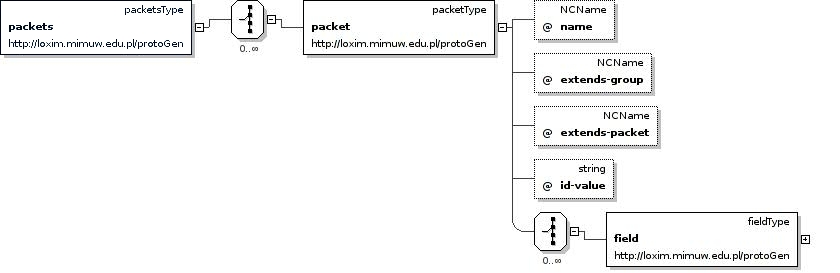
\includegraphics[scale=0.6]{xml/packets_level.jpg}
		\caption{Konstrukcja znacznika \znacznik{packet}}
	\end{figure}

	Element \znacznik{packets} grupuje znaczniki \znacznik{packet}, kt�re opisuj� pojedyncz� paczk�
	danych. Paczka danych sk�ada si� z p�l (patrz: \ref{field}), a ponadto jest
	opisana nast�puj�cymi atrybutami:
	\begin{description}
		\item[name] - Nazwa paczki
		\item[id-value] (atrybut opcjonalny) - Warto�� identyfikuj�ca paczk� (typu
		,,id-type''	z definicji grupy paczek). Je�li paczka nie posiada id-value - to jest
		traktowana jako ,,abstrakcyjna'', co oznacza, �e mo�e by� wykorzystana tylko
		jako paczka bazowa dla innych paczek.
		\item[extends-group] (atrybut opcjonalny) - nazwa grupy paczek, w kt�rej si�
		znajduje si� paczka zdefiniowana w polu ,,extends-packet''.  
		\item[extends-packet] (atrybut opcjonalny) - nazwa paczki z grupy
		''extends-group'', kt�r� deklarowana w�a�nie paczka rozszerza (o dodatkowe pola). 
	\end{description}
	

\subsubsection{\znacznik{field}} \label{field}
	\begin{figure}[hbt]
		\centering
			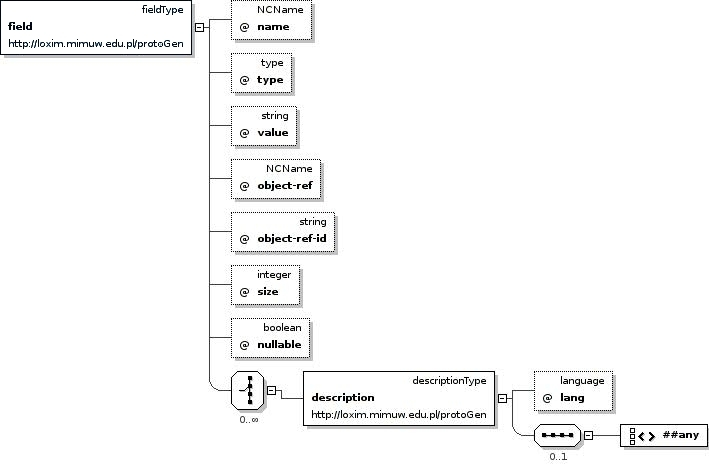
\includegraphics[scale=0.70]{xml/field_level.jpg}
		\caption{Konstrukcja znacznika \znacznik{fields}}
	\end{figure}

	Znacznik \znacznik{field} opisuje pojedyncze pole paczki. Podelementem znacznika \znacznik{field}
	mo�e by� znacznik \znacznik{description} (patrz: \ref{description}). Atrybutami znacznika
	field niezale�nie od typu tego pola s�:
	\begin{description}
		\item[name] - Nazwa pola
		\item[type] - Typ pola (patrz: \ref{typy})
	\end{description}

	Pozosta�e atrybuty zale�� od typu pola:
	\begin{itemize}
	\item Dla typ�w prostych dost�pny jest dodatkowo atrybut ,,value'' mog�cy
	zawiera� domy�ln� zawarto�� pola. 

	\item Dla typ�w: string, sstring, varuint dost�pny jest atrybut ''nullable''
	(przyjmuj�cy warto�ci true lub false), �wiadcz�cy o tym, czy dopuszczalna jest
	zawarto�� NULL dla tego pola. 
	
	\item Dla typ�w: string i sstring dost�pny jest atrybut size zawieraj�cy
	maksymaln� dopuszczaln� d�ugo�� napisu. 
	\end{itemize}
	
	Ponadto nast�puj� typy z�o�one wymagaj� szczeg�lnego om�wienia:
	\begin{description}
		\item[enum] - Pole zawiera jedn� z warto�ci z listy wyboru. Atrybut
		,,object-ref'' wskazuj� na nazw� odpowiedniego ,,enuma'' (patrz: \ref{enum}).
		Pole b�dzie serializowane jako typ ca�kowitoliczbowy wskazany w definicji
		,,enuma'' o warto�ci odpowiadaj�cej ,,id'' wybranego elementu z tej listy
		wyboru.
		\item[enum-map] \label{enum-map} - Pole zawiera bitow� map� warto�ci w listy
		wyboru. Atrybut ,,object-ref'' wskazuj� na nazw� odpowiedniego ,,enuma'' (patrz: \ref{enum}).
		Pole b�dzie serializowane jako typ ca�kowitoliczbowy wskazany w definicji
		,,enuma'' o warto�ci odpowiadaj�cej sumie ,,id'' wybranych elementu z tej
		listy wyboru.
		\item[package] - Pole zawiera cia�o (bez nag��wka) ca�ej innej paczki.
		Atrybut ,,object-ref'' wskazuj� na nazw� grupy paczek, a ,,object-ref-id'' na
 		nazw� konkretnej paczki nale��cej do tej grupy.
		\item[package-map] - Pole zawiera cia�o ca�ej innej paczki nale��cej
		do wskazanej grupy paczek, ale konkretny rodzaj paczki jest wyznaczony przez
		warto�� innego - uprzednio wymienionego pola. Zatem ,,object-ref'' wskazuj�
		na nazw� grupy paczek, a ,,object-ref-id'' na nazw� wcze�niej
		zdefiniowanego pola w bie��cej paczce - kt�re b�dzie zawiera�o
		identyfikator paczki, kt�ry ma zosta� w bie��cym polu wczytany/zapisany.
		O polu ,,package-map'' nale�y my�le� jak o polu ,,package'' z dynamicznie
		wyznaczanym konkretnym rodzajem paczki. 
    \end{description}
	
		
	
\subsubsection{\znacznik{description}}\label{description}
	Znacznik \znacznik{description} mo�e wyst�powa� w wielu miejscach specyfikacji
	protoko�u. S�u�y on do wygenerowania dokumentacji dotycz�cej wskazanego
	elementu protoko�u. Znacznik ten zawiera atrybut ,,lang'', kt�rego warto�ci�
	powinien by� kod j�zyka (kraju) - dwuliterowy, opisuj�cy j�zyk w kt�rym zosta�
	przeprowadzony opis. Zawarto�ci� znacznika mo�e by� dowolny tekstem tak�e
	wzbogacony o znaczniki j�zyka HTML. 

\subsubsection{Schemat (XML Schema) deskryptora protoko�u} \label{xml-schema}
\lstset{language=xml,tabsize=2,breaklines=true,showspaces=false,showstringspaces=false,showtabs=false}
\lstinputlisting{protogen.xsd}

\subsection{Proste typy danych}\label{typy}

	\subsubsection{Postanowienia og�lne}
		\begin{itemize}
          \item Je�li w spos�b szczeg�lny nie zaznaczono inaczej (a raczej
          nigdzie nie zaznaczono) wszystkie warto�ci zapisywane s� w formacie
          Big-endian.  W szczeg�lno�ci obejmuje to typy ca�kowitoliczbowe,
          rzeczywiste, oraz napisy w kodowaniu UTF-8 tak�e stosuj� kolejno��
          Big-endian. 
        \end{itemize}               

 	 \subsubsection{Ca�kowitoliczbowe: uint8,  sint8, uint16, sint16, int32,
 	 uint32, uint64, sint64} \label{integers}
		
	Pierwsza litera determinuje, czy mamy do czynienia z typem ze znakiem (u -
	unsigned), czy z typem bez znaku (s - signed).  Liczba na ko�cu wyra�a d�ugo��
	typu wyra�on� w bitach. 
	
	Typy s� kodowane oczywi�cie w kolejno�ci Big-endian. 
		
	\subsubsection{varuint - Ca�kowitoliczbowy z kompresj� (1,3,5 lub 9 bajt�w)}
		B�dzie to typ u�ywany g��wnie do oznaczania d�ugo�ci string�w i paczek. 
		
		Rozwi�zanie techniczne zosta�o zaczerpni�te z protoko�u serwera MySQL
		\cite{MySQL}.
		
		Idea jest taka, �e kr�tkie stringi ($<250$znak�w ) b�d� si�
		pojawia�y najcz�ciej i chcemy mie� najmniejszy narzut na zapisanie d�ugo�ci
		(jedno bajtowy). 
		
		Zatem semantyka pierwszego bajtu jest nast�puj�ca (w zale�no�ci od jego
		warto�ci)
		\begin{description}
			\item[0-249] Warto�� ta jest jednocze�nie warto�ci� wynikow�
			\item[250] Warto�� jest null'em (zostawiamy dla umo�liwienia stosowanie
			tego rozwi�zania z systemami relacyjnymi) 
			\item[251] Warto�� ta poprzedza 2-bajtowe (uint16) pole w warto�ci� w�a�ciw�
			\item[252] Warto�� ta poprzedza 4-bajtowe (uint32) pole z warto�ci� w�a�ciw�
			\item[253] Warto�� ta poprzedza 8-bajtowe (uint64) pole z warto�ci�
			w�a�ciw�. Nie nale�y jednak korzysta� z warto�ci wi�kszych ni� $2^{63}-1$
			(MAX\_SINT64), ze wzgl�du na to, �e w Javie nie s� obs�ugiwane 8 bajtowe
			typy bez znaku. 
        \end{description}
	
	\subsubsection{string - �a�cuchy tekstu}
	
	S�u�y do przesy�ania tekst�w. Teksty te musz� by� kodowane za pomoc� UTF-8. 
	
	Format warto�ci typu string jest nast�puj�cy:
	Najpierw idzie pole typu varuint - opisuj�ce d�ugo�� w bajtach nast�puj�cego
	potem ci�gu w UTF-8 (Big-endian). 
	
	\subsubsection{sstring - Kr�tki �a�cuch tekstu}
	Jest to tak naprawd� wariant typu string, 
	ale ograniczony do �a�cuch�w nie d�u�szych ni� 249 bajt�w.
	Czyli wtedy pole oznaczaj�ce d�ugo�� ma jeden bajt. 
	Jego wewn�trzna reprezentacja zupe�nie si� nie r�ni od typu
	string - zosta� on wyr�niony formalnie - ze wzgl�du na uproszczenie notacji 
	u�ywanej przy opisach format�w poszczeg�lnych paczek, a tak�e ze wzgl�d�w
	bezpiecze�stwa - gdy� pozwala zmniejszy� ryzyko typu DOS poprzez zaw�enie 
	wielko�ci danych, kt�re mog� by� zinterpretowane przez serwer. 
	
	\subsubsection{bytes - Dane binarne}\label{bytes}
	S�u�y do przesy�ania danych binarnych (tablic bajt�w).  
	
	Format warto�ci typu bytes jest nast�puj�cy:
	Najpierw jest wysy�ane pole typu varuint - opisuj�ce d�ugo�� w bajtach
	nast�puj�cego potem ci�gu bajt�w.
	
\newpage
\section{Dokumentacja wygenerowanego kodu}

\subsection{Wygenerowany kod dla j�zyka Java}
Generator protoko��w generuje kod w j�zyku Java w wersji nie starszej ni� Java
1.5, poniewa� korzysta z typ�w wyliczeniowych (enums) i szablon�w (generics). 

Zak�adaj�c, �e w metadanych opisu protoko�u dla j�zyka java zadeklarowano
packageName jako 'taki.sobie.protokol' (patrz: \ref{java-packageName}) to
zostanie wygenerowany nast�puj�cy projekt:

\subsubsection{pom.xml}
Pom.xml (Project Object Model) jest to plik opisuj�cy jak kompilowa� ten modu�
za pomoc� narz�dzia ,,Maven2''. Wskazuje on w szczeg�lno�ci biblioteki od
kt�rych projekt zale�y. 

\hyphenation{lo-xim}
\hyphenation{ja-va}
\hyphenation{pro-to-lib}

Modu� protoko�u wygenerowany przez ProtoGen zale�y od
biblioteki: \\pl.edu.mimuw.loxim.protogen.lang.java.protolib:java\_protolib, kt�ra
zawiera definicj� odpowiednich strumieni i klas bazowych (patrz:
\ref{java-protolib}).

Aby zbudowa� modu� wystarczy (zak�adaj�c, �e u�ytkownik posiada zainstalowanego Maven'a 2
\footnote{http://maven.apache.org/download.html}) wykona� polecenie ,,mvn package'' w
katalogu zawieraj�cym plik pom.xml. Wyniki procesu budowania zostan�
umieszczone w katalogu target. 

\subsubsection{Typy wyliczeniowe - enumy}
	Ka�dy ,,enum'' (typ wyliczeniowy) zostanie zapisany do katalogu
	./src/main/java/taki/sobie/protokol/enums jako ,,Enum'' j�zyka Java
	(wersja 1.5+).
	
	Typ ,,enum-map'' jest odwzorcowywany na odpowiedni ,,java.util.EnumSet$<$typ
	bazowy$>$'' (patrz: \ref{enum-map}).

\subsubsection{Grupy paczek} \label{java-PackagesFactory}

Paczki grupy g��wnej zostan� zapisane w folderze
./src/main/java/taki/sobie/protokol/packages, a paczki z pozosta�ych grup w 
folderze ./src/main/java/taki/sobie/protokol/packages\_$[$nazwa\_grupy$]$.

W ka�dym takim folderze powstanie tak�e klasa b�d�ca fabryk� paczek, 
kt�ra udost�pnia metod�:\\ 

public Package createPackage(long package\_id) throws
ProtocolException\\ 

Metoda ta tworzy paczk� w zale�no�ci od danego identyfikatora
paczki.

\subsubsection{Paczki} \label{java-paczki}

Dla ka�dej paczki zadeklarowanej w opisie protoko�u jest tworzona
odpowiednia klasa paczki. Wszystkie paczki rozszerzaj� nast�puj�c� klas�: 

\lstset{language=java,tabsize=2,breaklines=true,showspaces=false}
\lstinputlisting{src/Package.java}

Ponadto ka�da paczka zawiera nast�puj�ce elementy:
\begin{itemize}
  \item Publiczn� sta�� ID zawieraj�c� identyfikator paczki
  \item Bezparametrowy konstruktor paczki
  \item Konstruktor paczki, kt�ry przyjmuje wszystkie pola paczki jako swoje
  parametry
  \item Gettery i settery dla wszystkich p�l paczki 
\end{itemize}

\subsubsection{Testy}

Generator wygeneruje tak�e testy:
\begin{description}
  \item[./src/test/java/taki/sobie/protokol/tests/TestRunnerRec.java] - \\ 
  Klasa j�zyka java daj�ca si� uruchomi� (zawiera metod� main), kt�ra uruchamia
  proces, kt�ry otwiera gniazdo TCPIP na wskazanym porcie i sprawdza, czy
  otrzymane paczki s� zgodne z oczekiwanymi. Jedynym parametrem jaki mo�na
  przekaza� uruchamiaj�c t� klas� jest numer portu na kt�rym chcemy otworzy�
  gniazdo serwera. 
  
  Program ten mo�na wykorzystywa� do test�w komunikacji z implementacjami
  protoko�u dla innych j�zyk�w programowania.  
  
  \item[./src/test/java/taki/sobie/protokol/tests/TestRunnerSender.java] - \\
  Klasa j�zyka java daj�ca si� uruchomi� (zawiera metod� main), kt�ra uruchamia
  proces, kt�ry wysy�a na wskazany port na wskazanym serwerze paczki testowe.
  Uruchamiaj�c musimy przekaza� dwa parametry: nazw� hosta docelowego (lub
  adres IP), a tak�e port do kt�rego chcemy si� pod��czy�. 
  
  Program ten mo�na wykorzystywa� do test�w komunikacji z implementacjami
  protoko�u dla innych j�zyk�w programowania. 
   
  \item[./src/test/java/taki/sobie/protokol/tests/TestPackagesFactory.java] -\\
  Zawiera konstruktor wygenerowanych paczek testowych. Stanowi baz� dla
  innych test�w. 
  \item[./src/test/java/taki/sobie/protokol/tests/TestPackages.java] -\\
  Jest JUnitowym testem, kt�ry zapisuje wszystkie paczki testowe do
  strumienia, a nast�pnie je wszystkie wczytuje i sprawdza, czy paczki s�
  r�wne. Ten test jest u�ywany w fazie test�w w procesie budowania modu�u
  przez Maven 2. 
\end{description}

\subsubsection{java\_protolib}\label{java-protolib}
Biblioteka java\_protolib.jar jest plikiem, kt�ry zawiera niezale�n� od
konkretnego protoko�u definicj� podstawowych klas i interfejs�w.  

Poni�ej listujemy kluczowe klasy znajduj�ce si� w tej bibliotece: 

\begin{description}
\item[pl.edu.mimuw.loxim.protogen.lang.java.template.layers.ProtocolLayer0]~\\
Podstawowa klasa u�ywana w aplikacji do obs�ugi protoko�u. Zawiera metody
wysy�aj�ce przekazan� paczk�, a tak�e czekaj�c� i odczytuj�c� paczk�. Klasa
ponadto automatycznie odpowiada na paczk� ,,Ping'' paczk� ,,Pong''. 

\item[pl.edu.mimuw.loxim.protogen.lang.java.template.exception.ProtocolException]~\\
Wyj�tek rzucany gdy co� w protokole p�jdzie nie tak jak powinno. 

\item[pl.edu.mimuw.loxim.protogen.lang.java.template.pstreams.PackageOutputStream]~\\
Strumie� zak�adany na OutputStream'ie, kt�ry udost�pnia metod�
writePackage(Package p).

\item[pl.edu.mimuw.loxim.protogen.lang.java.template.pstreams.PackageInputStream]~\\
Strumie� zak�adany na InputStreamie, kt�ry udost�pnia metod� readPackage().

\item[pl.edu.mimuw.loxim.protogen.lang.java.template.streams.PackageOutputStreamWriter]~\\
Strumie� zak�adany na OutputStream'ie, kt�ry udost�pnia metody pozwalaj�ce
zapisa� proste typy danych (patrz \ref{typy}). 

\item[pl.edu.mimuw.loxim.protogen.lang.java.template.streams.PackageInputStreamReader]~\\
Strumie� zak�adany na InputStream'ie, kt�ry udost�pnia metody pozwalaj�ce
odczyta� proste typy danych (patrz \ref{typy}). 

\item[pl.edu.mimuw.loxim.protogen.lang.java.template.auth.AuthPassMySQL]~\\
Klasa pomocnicza oferuj�ca wsparcie dla przeprowadzania autoryzacji tak� metod�
jak robi to serwer bazy danych MySQL (,,Password Algorithm'' \cite{MYSQL})

\item[pl.edu.mimuw.loxim.protogen.lang.java.template.pstreams.PackagesFactory]~\\
Interfejs, kt�ry implementuj� wszystkie fabryki pakiet�w (patrz:
\ref{java-PackagesFactory})

\item[pl.edu.mimuw.loxim.protogen.lang.java.template.ptools.Package]~\\
Klasa bazowa dla wszystkich paczek.
\end{description}


\subsection{Wygenerowany kod dla j�zyka C++}
Kod dla j�zyka C++ jest samodzielny (jedyn� zale�no�ci� jest OpenSSL potrzeby
do dzia�aj�cej autoryzacji metod� zastosowan� w serwerze MySQL). Buduje si� go
za pomoc� polecenia make wydanego w katalogu ,,protocol''. 

\subsubsection{./make.defs}
Zawiera definicj� narz�dzi i bibliotek u�ywanych przez make. 

\subsubsection{Autentykacja - ./protocol/auth}
W tym folderze zawarte s� klasy pomocnicze potrzebne do 
przeprowadzenia autentykacji. Obecnie zaimplementowana jest tylko klasa
AuthPassMySQL wspieraj�ca autentykacj� metod� zastosowan� w serwerze MySQL i
wykorzystuj�ca sumy kontrolne SHA1. 

\subsubsection{Strumienie paczek - ./protocol/pstreams}

PackageOutputStream - Strumie� zak�adany na OutputStream;ie, kt�ry udost�pnia
metod� writePackage(Package* p).

PackageInputStream - Strumie� zak�adany na InputStream'ie, kt�ry udost�pnia
metod� readPackage() wczytuj�c� dany pakiet ze strumienia. 

\subsubsection{Typy wyliczeniowe - ./protocol/enums}
Ka�dy typ wyliczeniowy definiuje odpowiedni ,,enum'' j�zyka C++. 
Tworzony jest tak�e typ mapy (zawieraj�cy pole bitowe dla ka�dej warto�ci typu
wyliczeniowego). 

Ponadto tworzona jest tak�e fabryka umo�liwiaj�ca stworzenie instancji enuma lub
mapy enum�w na podstawie przekazanej warto�ci ca�kowitej, a tak�e zapisanie
enuma lub mapy enum�w jako liczb�. 

\subsubsection{Grupy pakiet�w}

Paczki grupy g��wnej zostan� zapisane w katalogu: ./protocol/packages, 
a grup nazwanych w ./protocol/packages\_$[$nazwa\_grupy$]$.

Dla ka�dej grupy zostanie wygenerowana klasa, b�d�ca fabryk� paczek w
zale�no�ci od przekazanego identyfikatora paczki. 

\subsubsection{Paczki}

Dla ka�dej paczki zostaje zaimplementowana klasa analogiczna do tej opisanej 
dla j�zyka Java (patrz: \ref{java-paczki}). 


\subsubsection{Testy - ./protocol/tests}
\begin{description}
	\item[./protocol/tests/TestRunnerRec]
	Uruchamia
  proces, kt�ry otwiera gniazdo TCPIP na wskazanym porcie i sprawdza, czy
  otrzymane pakiety s� zgodne z oczekiwanymi. Jedynym parametrem jaki mo�na
  przekaza� uruchamiaj�c t� klas� jest numer portu na kt�rym chcemy otworzy�
  gniazdo serwera. 
  
  Program ten mo�na wykorzystywa� do test�w komunikacji z implementacjami
  protoko�u w innych j�zykach programowania.  

	\item[./protocol/tests/TestRunnerSender]
	 Uruchamia
  proces, kt�ry wysy�a na wskazany port na wskazanym serwerze pakiety testowe.
  Uruchamiaj�c musimy przekaza� dwa parametry: nazw� hosta docelowego (lub
  adres IP), a tak�e port do kt�rego chcemy si� pod��czy�. 
  
  Program ten mo�na wykorzystywa� do test�w komunikacji z implementacjami
  protoko�u w innych j�zykach programowania. 

	\item[./protocol/tests/TestPackagesFactory]
  Jest to fabryka wygenerowanych pakiet�w testowych. Stanowi baz� dla
  innych test�w. 
\end{description}

\subsubsection{Gniazda - ./protocol/sockets}
Katalog zawiera prost�, obiektow� implementacj� gniazd. Jest ona wzorowana na
tej dost�pnej w j�zyku Java i umo�liwia �atwe u�ywanie gniazd sieciowych (zar�wno
serwerowych jak i klienckich) i otwieranie strumieni na nich. 

\begin{itemize}
\item ./protocol/sockets/TCPIPServerSocket
\item ./protocol/sockets/TCPIPServerSingleSocket
\item ./protocol/sockets/AbstractSocket
\item ./protocol/sockets/TCPIPClientSocket
\end{itemize}

\subsubsection{Strumienie ./protocol/streams}
Katalog zawiera elementarne, obiektowe implementacje strumieni - wzorowane na
j�zyku Java. 

\begin{description}
  \item[./protocol/streams/AbstractOutputStream,AbstractInputStream] -
  abstrakcyjne klasy bazowe dla strumieni
  \item[./protocol/streams/DescriptorInputStream,DescriptorOutputStream] -
  prosta implementacja strumieni oparta o zapis i odczyt ze wskazanego
  deskryptora systemu operacyjnego (pliku, urz�dzenia, gniazda sieciowego,
  ��cza). 
  \item[./protocol/streams/PriorityOutputStream]
  Klasa okalaj�ca (wrapper) strumienia wyj�ciowego, kt�ry udost�pnia dodatkow�
  metod� writePriority(char*), kt�ra przy wielu odwo�aniach do tego obiektu (z
  wielu w�tk�w) zostanie wykonana przed wykonaniami zapisu w zwyk�ych metodach
  write(char*) (odpowiednia synchronizacja na semaforach). 
\end{description}

\subsubsection{Warstwy protoko�u - ./protocol/layers/ProtocolLayer0}
Podstawowa klasa u�ywana w aplikacji do obs�ugi protoko�u. Zawiera metody
wysy�aj�ce przekazan� paczk�, a tak�e metod� czekaj�c� na i odczytuj�c� paczk�.
Klasa ponadto automatycznie odpowiada na paczki ,,Ping'' paczkami ,,Pong''. 

\subsubsection{Klasy pomocnicze}

\begin{description}
\item[./protocol/ptools/Endianness] -\\ 
Klasa zawiera metody u�atwiaj�ce konwersj� Little/Big Endian dla typ�w prostych
\item[./protocol/ptools/StringBufferStack] -\\
Klasa umo�liwia szybk� konstrukcje napis�w (bufor�w znak�w) poprzez sklejanie
napis�w (tablic znak�w). 
\item[./protocol/ptools/Package] -\\
Klasa bazowa dla wszystkich paczek
\item[./protocol/ptools/CharArray] -\\
Tablica znak�w z okre�lonym rozmiarem 
\item[./protocol/ptools/PackageBufferWriter] -\\
Klasa zawieraj�ca metody zapisuj�ce do danego strumienia typy proste. 
\item[./protocol/ptools/PackageBufferReader] -\\
Klasa zawieraj�ca metody odczytuj�ce z danego strumienia typy proste.
\end{description}

\subsubsection{Przyk�adowy kod u�ywaj�cy protok� po stronie serwera}

\lstset{language=C++,tabsize=2,breaklines=true,showspaces=false}
\lstinputlisting{src/UsageExampleServer.cpp}


\subsubsection{Przyk�adowy kod u�ywaj�cy protok� po stronie klienta}

\lstset{language=C++,tabsize=2,breaklines=true,showspaces=false}
\lstinputlisting{src/UsageExampleClient.cpp}

\newpage
\section{Dokumentacja programistyczna}
	\subsection{Architektura rozwi�zania}
		\subsubsection{Java}
ProtoGen zosta� napisany w j�zyku Java co umo�liwia u�ywanie go na wi�kszo�ci
platform sprz�towych i z wykorzystaniem wielu system�w operacyjnych.
 
		\subsubsection{Plexus - zorientowana na komponenty}
ProtoGen zosta� napisany w architekturze zorientowanej na komponenty. Do
zarz�dzania komponentami u�ywamy biblioteki Plexus (http://plexus.codehaus.org).
Z punktu widzenia u�ytkownika i programisty, zastosowanie tej architektury
umo�liwia stosunkowo �atwe dodanie obs�ugi nowego j�zyka generowanego kodu.
Wymaga ono jedynie stworzenia implementacji interfejsu:
,,pl.edu.mimuw.loxim.protogen.api.PartialLanguageGenerator'', a nast�pnie zadeklarowanie jej w
 lokalnym deskryptorze components.xml jar'a zawieraj�cego t� implementacj� jako: 

\lstset{language=xml,tabsize=2,breaklines=true,showspaces=false,showstringspaces=false,showtabs=false}
\lstinputlisting{src/components.xml}


W momencie, gdy taki jar znajdzie si� w classpath'ie uruchamianego ProtoGen'a,
to j�zyk ,,NowyJ�zyk'' b�dzie dost�pny jako jeden z docelowych j�zyk
dla generowanego kodu.

Reasumuj�c, g��wn� korzy�ci� zastosowania architektury zorientowanej na
komponenty, jest umo�liwienie zewn�trznym dostawcom dodawanie implementacji
nowych j�zyk�w bez �adnej ingerencji w dost�pny dotychczas kod. 
		
	\subsection{Proces budowania aplikacji}
	
	\begin{enumerate}
      \item Zainstalowa� Maven2 (http://maven.apache.org/download.html)
      \item Wej�� do katalogu g��wnego ProtoGen'a i wyda� polecenie ,,mvn
      clean package assembly:assembly''
      \item W podkatalogu ,,target/protogen-x.xx.xx-bin.dir'' b�dzie si�
      znajdowa�a wersja dystrybucyjna projektu. 
    \end{enumerate}
	
\subsection{Dalszy rozw�j} \label{roadmap}
	
	\subsubsection{Z�o�ona logika}
	Obecnie ProtoGen nie wspiera z�o�onej logiki w konstrukcji pakiet�w. Niemo�liwe jest warunkowanie istnienia pola w zale�no�ci od warto�ci innego pola,
	a tak�e tworzenia tablicy p�l. Obecnie ProtoGen przewiduje mo�liwo��
	nadpisania wygenerowanego kodu. W ten spos�b mo�na - nadpisuj�c kod obs�ugi
	odpowiedniej paczki - uzyska� obs�ug� dowolnie z�o�onej logiki.
		 	
	�eby zminimalizowa� konieczno�� wykorzystania takiego obej�cia, a tym
	samym uzyska� ,,pe�no��'' rozwi�zania przewidujemy w przysz�ych wersjach
	mo�liwo�� wprowadzenia nast�puj�cych atrybut�w do pola field (patrz:
	\ref{field}):
	\begin{description}
		\item[if-field] --- Zawiera nazw� pola z bie��cej paczki (wcze�niej
		zadeklarowanego), kt�rego warto�� b�dziemy por�wnywali do ,,if-value''. 
		\item[if-value] --- Je�eli zawarto�� pola o nazwie zadanej atrybutem ,,if-field''
		jest r�wna warto�ci ,,if-value'' to opisywane pole wyst�puje w tej paczce. W
		przeciwnym przypadku nie wyst�puje.
		\item[repeat] --- Zawiera nazw� pola ca�kowitoliczbowego, kt�re zawiera
		informacj� ile razy bie��ce pole jest powt�rzone.  
    \end{description}
	
	\subsubsection{Wi�cej j�zyk�w programowania}

	System jest przystosowany do rozszerzania o generatory do innych j�zyk�w
	programowania bez modyfikacji kodu �r�d�owego projektu bazowego. Dodanie
	obs�ugi nowego j�zyka programowania wymaga napisania komponentu systemu Plexus
	implementuj�cego interfejs
	,,pl.edu.mimuw.loxim.protogen.api.PartialLanguageGenerator''. 
	
	Oczywistym jest, �e dodanie generator�w do j�zyk�w programowania takich jak,
	C\#, Python, Ruby, PHP, Ocaml istotnie zwi�kszy u�yteczno�� tego projektu. 
	\subsubsection{Generowanie dokumentacji}
	Podobnie jak z dodatkowymi j�zykami programowania, wydaje si� istotn� z punktu
	widzenia u�ytkownika mo�liwo�� uzyskania aktualnej dokumentacji protoko�u.
	Cech� po��dan� jest by ProtoGen by� wstanie wygenerowa� dokumentacj� -
	najlepiej do wielu najpopularniejszych format�w (HTML, \LaTeX, PDF, ODF).
	
	By unikn�� r�cznej obs�ugi tych wszystkich format�w - wydaje si� uzasadnionym
	u�ycie narz�dzia typu Doxia (http://maven.apache.org/doxia), kt�re umo�liwia
	konwersje pomi�dzy wieloma formatami ,,bogatego'' tekstu.
	
	\subsubsection{Wsparcie dla wielu wersji pobocznych}
	
	Zar�wno definicj� paczki, jak i pola mo�na rozszerzy� o atrybut
	,,since-minor-version'', kt�ry b�dzie specyfikowa� od kt�rej wersji pobocznej
	protoko�u dane pole wyst�puje.
	
	Dodatkowo wymagamy, by kolejno��
	warto�ci ,,since-minor-version'' zgadza�a si� z kolejno�ci� p�l w paczce i by
	ka�de pole posiadaj�ce ten atrybut posiada�o tak�e zadeklarowan� warto��
	domy�ln� (pole ,,value''). Warunki te s� wystarczaj�ce, by zachowa� zgodno��
	protoko�u pomi�dzy r�nymi wersjami pobocznymi.  



\chapter{Zawarto�� p�yty} \label{spis-tresci-cd}

Do pracy zosta�a za��czona p�yta CD-ROM z zawarto�ci� zorganizowan� w
nast�puj�cy spos�b:

\begin{description}
	\item[./dokumenty/0. Praca magisterska - Piotr Tabor.pdf]
	\item[./dokumenty/1. Analiza starego protoko�u dla LoXiM.pdf]
	\item[./dokumenty/2. Dokumentacja nowego protoko�u dla LoXiM.pdf]
	\item[./dokumenty/3. Analiza mo�liwo�ci wykorzystania protoko�u LDAP dla SBQL
	DB.pdf]
	\item[./dokumenty/4. Dokumentacja generator protoko��w.pdf]
	\item[./dokumenty/src/] - Folder zawiera �r�d�owe pliki
	tex, a tak�e obrazki potrzebne do wygenerowanie w/w dokument�w przy pomocy
	systemu \LaTeX
	\item[./protogen/] - Folder zawiera pliki generatora protoko��w ,,ProtoGen'' 
	\item[./protogen/src/] - pliki �r�d�owe - do kompilacji za pomoc� narz�dzia
	,,Maven2''
	\item[./protogen/src/api/] - API generatora protoko��w z kt�rego korzystaj�
	generatory dla poszczeg�lnych j�zyk�w
	\item[./protogen/src/core/] - rdze� wykonywalne aplikacji ,,ProtoGen''
	\item[./protogen/src/langs/] - implementacje generacji kodu do r�nych
	j�zyk�w
	\item[./protogen/src/langs/cpp/] - do C++
	\item[/protogen/src/langs/java/] - do Javy
	\item[./protogen/src/langs/java\_protolib/] - biblioteka, z kt�rej
	korzysta wygenerowany kod dla Javy
	\item[./protogen/bin/] - skompilowana wersja generatora protoko��w
	,,ProtoGen''
	\item[./protogen/bin/*.jar] - biblioteki zawieraj�ce ,,ProtoGen'' i jego
	zale�no�ci
	\item[./protogen/bin/protoGen.sh] - skrypt uruchamiaj�cy ,,ProtoGen'' w
	systemach Unixowych (bash)
	\item[./protogen/bin/protoGen.bat] - skrypt uruchamiaj�cy ,,ProtoGen'' w
	systemach firmy Microsoft
	\item[./protogen/example/] - katalog zawiera zestaw danych
potrzebnych do wygenerowania protoko�u
	 \item[./protogen/example/over/]  - dla LoXiMa przy u�yciu za��czonego
	 generatora "ProtoGen"
	\item[./protogen/example/over/cpp/] - zestaw plik�w do nadpisania
przy generowaniu do C++ 
	\item[./protogen/example/over/java/] - zestaw plik�w do nadpisania przy
	generowaniu do Javy
	\item[./protogen/example/loxim2.xml] - opis XML protoko�u dla
LoXiMa
	\item[./protogen/example/run.sh] - skrypt, kt�ry uruchamia
generowanie kodu do C++ i Javy
	\item[./loxim\_protocol/] - katalog zawiera wygenerowane
	biblioteki na potrzeby systemu LoXiM:
	\item[./loxim\_protocol/cpp/] - w j�zyku C++ 
	\item[./loxim\_protocol/java/] - w j�zyku Java
	\item[./licencje] - katalog zawiera tre�ci licencji na kt�rych znajduje si�
	sama praca,a tak�e tych na kt�rych zosta�y wydane wykorzystywane w pracy
	komponenty i biblioteki.
\end{description}

%\chapter{Deskryptor protoko�u \loxim'a dla generatora
%protoko��w ,,ProtoGen~1.0''}\label{listing-loxim-xml}

%\lstset{language=xml,tabsize=2,breaklines=true,showspaces=false,showstringspaces=false,showtabs=false}
%\lstinputlisting{loxim2.xml}


\begin{thebibliography}{99}
	\addcontentsline{toc}{chapter}{Bibliografia}
	
	\bibitem[OSI]{OSI}OSI Reference Model ISO/IEC standard 7498-1:1994, ISO,
[20.05.2008] (http://standards.iso.org/ittf/PubliclyAvailableStandards/s020269\_ISO\_IEC\_7498-1\_1994(E).zip)
	
\bibitem[DoD]{DoD} Architectural Principles of the Internet, RFC 1958, B.
Carpenter, June 1996

\bibitem[MYSQL]{MySQL}MySQL Protocol - version 10. Ian Redfern,
[03.12.2006], (http://www.redferni.uklinux.net/mysql/MySQL-Protocol.html) 

\bibitem[PGSQL]{PostgreSQL}PostgreSQL Frontend/Backend Protocol - version.
PostgreSQL Fundation, [03.12.2006],
(http://developer.postgresql.org/pgdocs/postgres/protocol.html)

\bibitem[SBQL]{SBQL}Stack-Based Approach (SBA) and Stack-Based Query Language
(SBQL). Kazimierz Subieta, [03.12.2006], (http://www.sbql.pl)

\bibitem[TDS]{TDS}TDS Protocol Documentation. FreeTDS, [10.12.2006],
(http://www.freetds.org/tds.html)

\bibitem[UTS10]{UTS10}Unicode Technical Standard \#10 Unicode Collation
Algorithm. Mark Davis, Ken Whistler, [29.05.2008], (http://www.unicode.org/reports/tr10/)

\bibitem[ISO8601]{ISO8601}ISO 8601 - Numeric representation of Dates and Time,
ISO, [29.05.2008],
(http://www.iso.org/iso/support/faqs/faqs\_widely\_used\_standards/ widely\_used\_standards\_other/date\_and\_time\_format.htm)

\bibitem[ASN1]{ASN1} Communication between heterogeneous systems, Olivier
Dubuisson, 2008, (http://www.oss.com/asn1/bookreg2.html)

	\bibitem[LDAP]{LDAP}Lightweight Directory Access Protocol (LDAP): Technical
Specification Road Map, K. Zeilenga, Ed.[06.2006]
%\bibitem[SBQL]{SBQL}Stack-Based Approach (SBA) and Stack-Based Query Language
%(SBQL). Kazimierz Subieta, [03.12.2006], (http://www.sbql.pl)
\bibitem[RFC4511]{RFC4511} Sermersheim, J., Ed., "Lightweight Directory Access
                 Protocol (LDAP): The Protocol", RFC 4511, June 2006.
\bibitem[RFC4512]{RFC4512} Zeilenga, K., "Lightweight Directory
   Access Protocol (LDAP): Directory Information Models", RFC 4512, June
                 2006.
\bibitem[RFC4513]{RFC4513} Harrison, R., Ed., "Lightweight Directory
   Access Protocol (LDAP): Authentication Methods and Security
                 Mechanisms", RFC 4513, June 2006.
\bibitem[RFC4514]{RFC4514} Zeilenga, K., Ed., "Lightweight Directory
   Access Protocol (LDAP): String Representation of Distinguished
                 Names", RFC 4514, June 2006.
\bibitem[RFC4515]{RFC4515} Smith, M., Ed. and T. Howes, "Lightweight
   Directory Access Protocol (LDAP): String Representation of Search
                 Filters", RFC 4515, June 2006.
\bibitem[RFC4516]{RFC4516} Smith, M., Ed. and T. Howes, "Lightweight
   Directory Access Protocol (LDAP): Uniform Resource Locator", RFC
                 4516, June 2006.
\bibitem[RFC4517]{RFC4517}  Legg, S., Ed., "Lightweight Directory
   Access Protocol (LDAP): Syntaxes and Matching Rules", RFC 4517, June
                 2006.
\bibitem[RFC4519]{RFC4518} Zeilenga, K., "Lightweight Directory
   Access Protocol (LDAP): Internationalized String Preparation", RFC
                 4518, June 2006.
\bibitem[RFC4519]{RFC4519} Sciberras, A., Ed., "Lightweight
   Directory Access Protocol (LDAP): Schema for User Applications", RFC
                 4519, June 2006.
\bibitem[RFC5420]{RFC4520} Zeilenga, K., "Internet Assigned Numbers
   Authority (IANA) Considerations for the Lightweight Directory
                 Access Protocol (LDAP)", BCP 64, RFC 4520, June 2006.
\bibitem[RFC4521]{RFC4521} Zeilenga, K., "Considerations for LDAP
   Extensions", BCP 118, RFC 4521, June 2006.
\bibitem[X.500]{X.500} [X.500]       International Telecommunication Union -
                 Telecommunication Standardization Sector, "The
                 Directory -- Overview of concepts, models and
                 services", X.500(1993) (also ISO/IEC 9594-1:1994).
\bibitem[X.501]{X.501} International Telecommunication Union -
                 Telecommunication Standardization Sector, "The
                 Directory -- Models", X.501(1993) (also ISO/IEC 9594-
                 2:1994).
\bibitem[X.511]{X.511} International Telecommunication Union -
                 Telecommunication Standardization Sector, "The
                 Directory: Abstract Service Definition", X.511(1993)
                 (also ISO/IEC 9594-3:1993).

	
\end{thebibliography}

\end{document}


%%% Local Variables:
%%% mode: latex
%%% TeX-master: t
%%% coding: latin-2
%%% End:
